% Este archivo es parte de la memoria del proyecto fin de carrera
% de Manuel López Urbina. Protegida bajo la licencia GFDL.
% Para más información, la licencia completa viene incluida en el
% fichero fdl-1.3.tex
% Fuente tomada de la plantilla LaTeX para
% la realización de Proyectos Final de Carrera de Pablo Recio Quijano.
% Copyright (C) 2009 Pablo Recio Quijano
% Copyright (C) 2012 Manuel López Urbina

%-----------------------------------------------------------------------
% ---- Memoria del proyecto fin de carrera de Manuel López Urbina -----

% Basado en la plantilla para memorias de proyectos fin de carrera
% realizada por Pablo Recio Quijano y Noelia Sales Montes
% ----------------------------------------------------------------------

\documentclass[a4paper,12pt]{book}

\usepackage{./estilos/estiloBase}
\usepackage{./estilos/colores}
\usepackage{./estilos/comandos}

\graphicspath{{./imagenes/}}

\usepackage{appendix}%
%\headheight = 15 pt%
\headsep = 27 pt%
\clearpage{\pagestyle{empty}\cleardoublepage}%

%\setcounter{secnumdepth}{3}
%\setcounter{tocdepth}{3}

%\usepackage{float}
%\usepackage[titletoc]{appendix}
%\newfloat{imagencontexto}{ht}{lop}
%\floatname{imagencontexto}{ImagenConTexto}

%\setlength{\parskip}{1ex plus 0.5em minus 0.2ex}




%\usepackage{color} % Paquete de colores
%\usepackage{fancyvrb}

%\usepackage{fancyvrb}
%\usepackage[utf8]{inputenc}


\begin{document}

\renewcommand{\labelitemi}{$\bullet$}%
\renewcommand{\labelitemii}{$\diamond$}%
\renewcommand{\figurename}{Figura}
\renewcommand{\listfigurename}{Índice de figuras}
\renewcommand{\tablename}{Tabla}
\renewcommand{\listtablename}{Índice de tablas}
\newcommand{\icontext}[3]{\raisebox{-#1\height}{\includegraphics[scale=#2]{#3}}}


% Este archivo es parte de la memoria del proyecto fin de carrera
% de Manuel López Urbina. Protegida bajo la licencia GFDL.
% Para más información, la licencia completa viene incluida en el
% fichero fdl-1.3.tex
% Fuente tomada del PFC 'libgann' de Francisco Javier Vázquez Púa.
% Fuente tomada de la plantilla LaTeX para
% la realización de Proyectos Final de Carrera de Pablo Recio Quijano.
% Copyright (C) 2008 Francisco Javier Vázquez Púa
% Copyright (C) 2009 Pablo Recio Quijano
% Copyright (C) 2009 Diego Barrios Romero

% Copyright (C) 2012 Manuel López Urbina

\pagestyle{empty}
\begin{titlepage}

  \begin{center}

    
\includegraphics[scale=0.2]{logo_uca.png} \\

    \vspace{2.0cm}

    \LARGE{\textbf{ESCUELA SUPERIOR DE INGENIERÍA}} \\

    \vspace{1.0cm}

    \Large{\textbf{INGENIERÍA TÉCNICA EN INFORMÁTICA DE SISTEMAS}} \\

    \vspace{3.0cm}

    \Large{OpenTSR:\\ Vehículo reconocedor de señales de tráfico} \\

    \vspace{2.0cm}

    \Large{Manuel López Urbina} \\

    \vspace{0.5cm}

    \large{\today}

  \end{center}
\end{titlepage}

\cleardoublepage

% Este archivo es parte de la memoria del proyecto fin de carrera
% de Manuel López Urbina. Protegida bajo la licencia GFDL.
% Para más información, la licencia completa viene incluida en el
% fichero fdl-1.3.tex
% Fuente tomada del PFC 'libgann' de Francisco Javier Vázquez Púa.
% Fuente tomada de la plantilla LaTeX para
% la realización de Proyectos Final de Carrera de Pablo Recio Quijano.
% Copyright (C) 2008 Francisco Javier Vázquez Púa
% Copyright (C) 2009 Pablo Recio Quijano
% Copyright (C) 2009 Diego Barrios Romero

% Copyright (C) 2012 Manuel López Urbina


\pagestyle{empty}
\begin{center}

  
\includegraphics[scale=0.2]{logo_uca.png} \\

  \vspace{2.0cm}

  \Large{ESCUELA SUPERIOR DE INGENIERÍA} \\

  \vspace{1.0cm}

  \large{INGENIERO TÉCNICO EN INFORMÁTICA DE SISTEMAS} \\

  \vspace{2.0cm}

  \large{OpenTSR: \\Vehículo reconocedor de señales de tráfico} \\

  \vspace{1.0cm}

\end{center}

\begin{itemize}
\item \large{Departamento: Ingeniería en Automática, Electrónica, Arquitectura y Redes de Computadores}
\item \large{Director del proyecto: Arturo Morgado Estévez}
\item \large{Autor del proyecto: Manuel López Urbina}
\end{itemize}

\vspace{1.0cm}

\begin{flushright}
  \large{Cádiz, \today} \\

  \vspace{2.5cm}

  \large{Fdo: Manuel López Urbina}
\end{flushright}

\cleardoublepage

\frontmatter % Introducción, índices ...
\pagestyle{plain}
% Este archivo es parte de la memoria del proyecto fin de carrera
% de Manuel López Urbina. Protegida bajo la licencia GFDL.
% Para más información, la licencia completa viene incluida en el
% fichero fdl-1.3.tex

% Copyright (C) 2012 Manuel López Urbina

\section*{Agradecimientos}

Este proyecto significa la culminación de mi carrera, por lo que me gustaría dedicárselo a todas las personas que me han ayudado a conseguir acabarla.\\

En primer lugar me gustaría agradecerle a mi familia el apoyarme y ayudarme durante estos años, y el esfuerzo que han hecho para que yo haya podido llegar a este momento.\\

Agradecimientos a D. Arturo Morgado por su ayuda y dedicación durante la realización y dirección de este proyecto, así como su carácter amable y servicial que han hecho más ameno el trabajo realizado.\\

También me gustaría agradecérselo a mis compañeros, con los que tantos ratos inolvidables he pasado, y que tanto me han ayudado, entre ellos, agradecimientos a Noelia Sales Montes por la elaboración del logotipo del proyecto y a Andrés Francisco Aparicio por proporcionar un nombre al mismo. A Moisés Gautier Gómez por ser un excelente compañero tras numerosas horas de trabajo en el aula de robótica.\\

Por último quiero dedicarle este proyecto a todos los estudiantes de informática, en especial a todos los amantes del fascinante mundo de la robótica, a los que espero que mi trabajo les sea de utilidad.\\

\cleardoublepage

\section*{Licencia}

Este documento ha sido liberado bajo Licencia GFDL 1.3 (GNU Free Documentation License). Se incluyen los términos de la licencia en inglés al final del mismo.\\

Copyright (c) 2012 Manuel López Urbina.\\

Permission is granted to copy, distribute and/or modify this document under the terms of the GNU Free Documentation License, Version 1.3 or any later version published by the Free Software Foundation; with no Invariant Sections, no Front-Cover Texts, and no Back-Cover Texts. A copy of the license is included in the section entitled "GNU Free Documentation License".\\

\cleardoublepage


\cleardoublepage

\tableofcontents
\listoffigures
\listoftables

\mainmatter % Contenido en sí ...
%\pagestyle{plain}

\pagestyle{fancy}%
\fancyhead[LE,RO]{\rightmark}%
\fancyhead[LO,RE]{\slshape \leftmark}%
\fancyfoot[C]{\thepage}

% Este archivo es parte de la memoria del proyecto fin de carrera
% de Manuel López Urbina. Protegida bajo la licencia GFDL.
% Para más información, la licencia completa viene incluida en el
% fichero fdl-1.3.tex

% Copyright (C) 2012 Manuel López Urbina

\chapter{Introducción}
\label{chap:introducción}

\section{Introducción y antecedentes}

En la actualidad, los robots comerciales e industriales son ampliamente utilizados y realizan tareas de forma más exacta o más barata que los humanos. También se les utiliza en trabajos demasiado sucios, peligrosos o tediosos. Los robots son muy utilizados en plantas de fabricación, montaje y embalaje, en transporte, en exploraciones en la Tierra y en el espacio, cirugía, armamento, investigación en laboratorios y en la producción en masa de bienes industriales o de consumo. Otras aplicaciones incluyen la limpieza de residuos tóxicos, minería, búsqueda y rescate de personas y localización de minas terrestres, en definitiva, la robótica está presente en prácticamente cualquier ámbito de la actualidad.\\

Por otra parte, ninguno de los sistemas robóticos actuales podrían ser funcionales sin un software adecuado para automatización de tareas, siendo esencial una correcta sincronización entre los diferentes elementos hardware y software implicados con la finalidad de garantizar un correcto funcionamiento del conjunto robótico.\\

Centrándonos en lo anterior y aplicándolo en el campo de la automoción, ocasiona que en la actualidad se empleen importantes esfuerzos por parte de grupos investigadores y fabricantes de automóviles para dotar sus vehículos de los elementos necesarios para proporcionar a sus vehículos de un sistema de conducción autónoma. Campo en la actualidad en pleno desarrollo y presentando multitud problemas aún por resolver.\\

Entre los problemas existentes en los sistemas de conducción autónoma destaca su escasa adaptabilidad en carreteras reales donde existen multitud de imperfecciones, como pueden ser el desgaste o la falta de las señales viales, falta de iluminación o existencia de señalización provisional no fija como las indicadoras de obras en la vía. Estas circunstancias especiales impiden el correcto funcionamiento de los vehículos de dentro de unos niveles de seguridad mínimos aceptables para su implantación en carreteras transitables junto con vehículos conducidos de modo tradicional.\\

La problemática actual presentada, junto con que robótica y automoción son mis dos pasiones, hizo que me lanzara a la elaboración de este proyecto que unifica ambos campos anteriormente citados.\\

Así surgió \emph{OpenTSR}.\\

Se trata de un vehículo controlado vía WiFi dotado de una cámara de vídeo la cual visualiza su en torno en busca de aquellas señales de tráfico presentes y actuar en consecuencia.\\

\begin{figure}[H]
  \begin{center}
    
\includegraphics[scale=0.3]{lente1.png}
  \end{center}
  \label{fig:logo}
 \caption{Logo OpenTSR \protect\footnotemark.}
\end{figure}

\footnotetext{Logotipo elaborado por Noelia Sales Montes para el proyecto OpenTSR.}

\emph{OpenTSR} (que será el nombre del sistema resultante) será una combinación de un elemento hardware (vehículo entre otros) y software (consola de control) surgido como una aproximación a la solución de los citados problemas.\\

\section{Objetivos}
\label{sec:objetivos}

El objetivo principal del proyecto es elaborar un software de detección de señales de tráfico mediante el análisis de las imágenes obtenidas a partir de una cámara. Dicho software irá asociado a un vehículo dotado de una cámara para permitir la visualización del terreno además de ser capaz de reconocer las señales de tráfico mostrando en el ordenador la última señal reconocida. Por otra parte, permitirá al vehículo actuar en consecuencia a la señal detectada. En definitiva se desea dotar al vehículo de un sistema de conducción autónoma \footnote{En la sección \ref{sec:def-vehículo-autónomo} referente a conceptos básicos se incluye la definición de vehículo autónomo.} a partir de señales de tráfico.\\

El sistema a desarrollar, por tanto, dispondrá de dos modos de funcionamiento, el primero de ellos proporciona una conducción a gusto del usuario, el cual podrá controlar a su antojo el vehículo por el entorno que le rodea mediante un joystick o haciendo uso de las teclas del teclado de un ordenador. En el segundo modo de funcionamiento, el vehículo actuará automáticamente según las señales de tráfico detectadas por la cámara, siendo capaz de ajustar velocidad o realizar giros y paradas de manera automática según los elementos visionados a través de la cámara.\\

\section{Acerca de este documento}

El documento se ha sido elaborado en un lenguaje sencillo y claro para permitir que un estudiante universitario de cualquier Ingeniería Informática pueda comprender los contenidos sin apenas dificultad añadida.\\

Este documento se organiza en los siguientes capítulos:\\

\begin{itemize}

\item En el capítulo \ref{chap:introducción}, Introducción, se comentan las razones que han motivado la creación de este proyecto, así como el propósito del mismo.

\item En el capítulo \ref{chap:conceptos-básicos}, Conceptos básicos, se incluyen definiciones de aquellos conceptos considerados de interés para la correcta comprensión del contenido de la presente memoria.

\item En el capítulo \ref{chap:herramientas}, Herramientas utilizadas, se realiza una descripción de las diferentes elementos hardware y software empleados durante el desarrollo del proyecto y necesarios para la utilización del mismo.

\item En el capítulo \ref{chap:organización-temporal}, Organización temporal, se recoge todo lo que concierne a la distribución y duración de cada una de las tareas llevadas a cabo durante el desarrollo del proyecto que el presente documento describe.

\item En el capítulo \ref{chap:dispositivos-hardware}, Configuración y montaje de los dispositivos hardware, se explica el proceso seguido para la correcta integración de los dispositivos hardware empleados describiendo la interconexión entre ellos así como su configuración. 

\item En el capítulo \ref{chap:desarrollo-software}, Desarrollo software, se realiza un análisis sobre la metodología empleada para el desarrollo software, describiendo los modelos de ciclo de vida utilizados, la descripción de los requisitos funcionales junto con el diagrama de casos de uso.

\item En el capítulo \ref{chap:reconocimiento}, Software de reconocimiento, se hace una descripción explicando los diferentes aspectos y elementos de cada uno de los prototipos desarrollados junto con los problemas encontrados y soluciones adoptadas.

\item En el capítulo \ref{chap:software-de-control}, Software de control, se describe cómo se ha llevado a cabo la comunicación ordenador-vehículo a nivel software.

\item En el capítulo \ref{chap:interfaz-gráfica}, Interfaz gráfica, se recogen aquellos aspectos técnicos de interés referentes a la elaboración de la interfaz gráfica.

\item En el capítulo \ref{chap:manual-usuario}, Guía de usuario, se describen los diferentes aspectos necesarios para la correcta utilización del conjunto software y hardware de los que se compone el presente proyecto.

\item En el capítulo \ref{chap:conclusiones}, Conclusiones, se hace mención de las conclusiones obtenidas tras la realización del proyecto además de las posibles mejoras aplicables.

\item En el capítulo Anexos \ref{chap:anexos}, aparecen los manuales de instalación del software que ha sido necesario para la realización del proyecto.

\end{itemize}


% Este archivo es parte de la memoria del proyecto fin de carrera
% de Manuel López Urbina. Protegida bajo la licencia GFDL.
% Para más información, la licencia completa viene incluida en el
% fichero fdl-1.3.tex

% Copyright (C) 2012 Manuel López Urbina

\chapter{Conceptos básicos}
\label{chap:conceptos-básicos}

\section{Vehículo Autónomo}
\label{sec:def-vehículo-autónomo}

Un vehículo autónomo, es un vehículo capaz de cumplir con las capacidades de transporte llevadas a cabo por los humanos en un vehículo tradicional por sí mismo. Dicho vehículo es capaz de detectar los diferentes elementos de su entorno permitiendo un desplazamiento por sí mismo. Un ser humano puede elegir un destino, siendo innecesario realizar ninguna otra operación mecánica en el vehículo.\\

Los Vehículos autónomos perciben el mundo que le rodea gracias a la utilización de multitud de sensores tales como radares, GPS y visión por computador, siendo esta última la principal temática de este proyecto. Posteriormente un sistema avanzados de control interpretará la información para identificar las rutas adecuadas de navegación, así como los obstáculos y la señalización correspondiente. Dichos vehículos suelen actualizar sus mapas basados en la información sensorial, de forma que permiten la navegación a través de entornos desconocidos.

\section{Inteligencia artificial}   
\label{sec:def-inteligencia-artificial}

La inteligencia artificial (IA) se define como la capacidad de un dispositivo para llevar a cabo funciones que normalmente se asocian con la inteligencia humana, tales como el razonamiento y la optimización de la experiencia. La IA es la rama de la informática que trata de aproximar los resultados del razonamiento humano mediante la organización y manipulando conocimiento de los hechos y heurísticos. Las áreas de actividad de AI incluyen los sistemas expertos, la comprensión del lenguaje natural, reconocimiento de voz, la visión artificial y la robótica.

\section{Visión artificial}
\label{def:visión-artificial}

La visión artificial, también conocida como visión por computador, es un subcampo perteneciente a la inteligencia artificial\footnote{Definición de \emph{inteligencia artificial} incluida en la sección \ref{sec:def-inteligencia-artificial}.}. El propósito de la visión artificial es programar un computador para que \emph{entienda} una escena o las características de una imagen.\\

Los objetivos típicos de la visión artificial incluyen:

\begin{itemize}
\item La detección, segmentación, localización y reconocimiento de objetos en imágenes (por ejemplo, caras humanas).
\item La evaluación de resultados (por ejemplo, segmentación, registro).
\item Registro de diferentes imágenes de una misma escena u objeto, es decir, hacer concordar un mismo objeto en diversas imágenes.
\item Seguimiento de un objeto en una secuencia de imágenes.
\item Mapeo de una escena para generar un modelo tridimensional de la escena; este modelo podría ser usado por un robot para navegar por la escena.
\item Búsqueda de imágenes digitales por su contenido.
\end{itemize}

Estos objetivos se consiguen por medio de reconocimiento de patrones\footnote{Definición de \emph{reconocimiento de patrones} disponible en la sección \ref{def:reconocimiento-de-patrones}.}, aprendizaje estadístico, geometría de proyección, procesamiento de imágenes, teoría de grafos y otros campos. En este proyecto nos centraremos en técnicas propias del reconocimiento de patrones.

\section{Reconocimiento de patrones}
\label{def:reconocimiento-de-patrones}

El reconocimiento de patrones, también llamado lectura de patrones, identificación de figuras y reconocimiento de formas, consiste en el reconocimiento de patrones de señales. Los patrones son obtenidos a partir de procesos de segmentación, extracción de características y descripción para que cada objeto quede representado de manera lo más representativa posible por una colección de descriptores. El sistema de reconocimiento debe asignar a cada objeto su categoría o clase (conjunto de entidades que comparten alguna característica que las hacen diferentes al resto). Para poder reconocer los patrones se siguen tres procesos principales:\\

\begin{itemize}
 \item Adquisición de datos.
 \item Extracción de características.
 \item Toma de decisiones.
\end{itemize}

La esencia del reconocimiento de patrones es la clasificación, un ejemplo práctico de clasificación puede ser la clasificación de imágenes digitales de letras en las clases de la \emph{A} a la \emph{Z} dependiendo de sus píxeles u otras situaciones que podamos extraer.\\

\begin{figure}[H]
  \begin{center}
    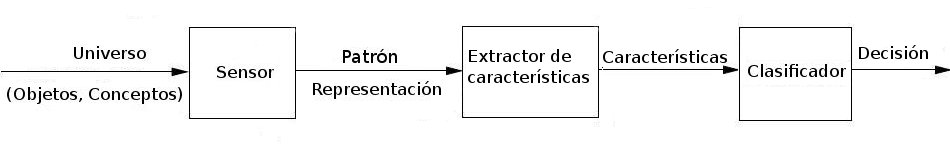
\includegraphics[scale=0.6]{Pattern.jpg}
  \end{center}
  \caption{Componentes básicos de un sistema de reconocimiento de patrones.}
  \label{Componentes-basicos-rp}
\end{figure}


\subsection {Aplicaciones}

Los sistemas de reconocimiento de patrones tienen multitud de aplicaciones. Algunas de las más relevantes y utilizadas actualmente son:\\

\begin{itemize}
\item Previsión meteorológica: poder clasificar datos meteorológicos según diversos patrones, y con el conocimiento a priori que tenemos de las diferentes situaciones que pueden aperecer nos permite crear mapas de predicción automática.
\item Reconocimiento de caracteres escritos a mano o a máquina: es una de las utilidades más populares de los sistemas de reconocimiento de patrones ya que los símbolos de escritura son fácilmente identificables.
\item Reconocimiento de voz: el análisis de la señal de voz se utiliza actualmente en muchas aplicaciones, un ejemplo claro son los teleoperadores informáticos.
\item Aplicaciones en medicina: análisis de biorritmos, detección de irregularidades en imágenes de rayos-x, detección de células infectadas, marcas en la piel...
\item Reconocimiento de huellas dactilares: utilizado y conocido por la gran mayoría, mediante las huellas dactilares todos somos identificables y con programas que detectan y clasifican las coincidencias, resulta sencillo encontrar correspondencias.
\item Reconocimiento de caras: utilizado para contar asistentes en una manifestación o simplemente para detectar una sonrisa, ya hay diferentes cámaras en el mercado con esta opción disponible.
Interpretación de fotografías aéreas y de satélite: gran utilidad para propuestas militares o civiles, como la agricultura, geología, geografía, planificación urbana...
\item Predicción de magnitudes máximas de terremotos.
\item Reconocimiento de objetos: con importantes aplicaciones para personas con discapacidad visual.
\item Reconocimiento de música: identificar el tipo de música o la canción concreta que suena.
\end{itemize}


\section {Modelos de color}
\label{def:modelos-color}

El color, como cualquier otro recurso, también tiene su técnica y se enecuntra sometido a ciertas leyes, y según la aplicación que se desea, se trabaja con distintos modelos de color. Los modelos de color describen los colores que se ven en las imágenes digitales e impresas y el trabajo con ellos.\\

Los modelos de color permiten, además de establecer un espacio único común a todos los equipos que realizan operaciones de adquisición y reproducción de color, permiten simular cómo lucirá la imagen y su color en otro dispositivo; así por ejemplo, podemos ver en la pantalla del computador cómo saldrá la imagen impresa en el papel, después de que haya pasado por las tintas que se usan normalmente en prensa y con diferentes papeles, permitiendo un trabajo de edición de imagen y color mucho más sencilla y fiel a los resultados finales.\\

Cada modelo de color como, por ejemplo, RGB, CMYK o HSV representa un método diferente (y por lo general, numérico) de descripción de los colores.\\

A continuación se describen los aquellos modelos de mayor importancia:

\subsection{Modelo RGB}

La descripción RGB, del inglés Red, Green, Blue, de un color hace referencia a la composición del color en términos de la intensidad de los colores primarios con que se forma: el rojo, el verde y el azul. Este modelo de color está basado en la síntesis aditiva, permitiendo representar un color mediante la mezcla por adición de los tres colores de luz primarios de los que se compone. El modelo de color RGB no define por sí mismo lo que significa exactamente rojo, verde o azul, por lo que los mismos valores RGB pueden mostrar colores notablemente diferentes en diferentes dispositivos que usen este modelo de color. Aunque utilicen un mismo modelo de color, sus espacios de color pueden variar considerablemente.
Con el fin de indicar con qué proporción se mezcla cada color, se asigna un valor numérico a cada uno de los colores primarios, de manera que, por ejemplo, el valor 0 significa que ese color no interviene en la mezcla y, a medida que ese valor aumenta, se entiende que aporta más intensidad al conjunto. Aunque el intervalo de valores podría ser cualquiera (valores reales entre 0 y 1, valores enteros entre 0 y 37, etc.), aunque en la mayoría de ocasiones cada color primario es codificado con un byte (8 bits). Así, de manera usual, la intensidad de cada una de las componentes se mide con una escala del 0 al 255.\\

Por lo tanto, el rojo es obtenido con (255,0,0), el verde con (0,255,0) y el azul con (0,0,255), siendo para los tres casos un color monocromático. La ausencia de color, lo que identificamos como el color negro, se obtiene cuando las tres componentes son 0, (0,0,0).\\

La combinación de dos colores a nivel 255 con un tercero en nivel 0 da lugar a la obtención de los tres colores intermedios. De esta forma el amarillo es (255,255,0), el cian (0,255,255) y el magenta (255,0,255).\\

Finalmente, el color blanco se forma con los tres colores primarios a su máximo nivel (255,255,255).\\

\begin{figure}[H]
  \begin{center}
    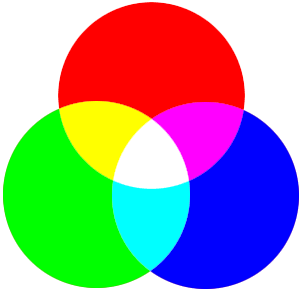
\includegraphics[scale=0.3]{modelo-RGB.png}
  \end{center}
  \caption{Modelo de color RGB.}
  \label{modelo-RGB}
\end{figure}

\subsection{Modelo HSV}

El modelo HSV, del inglés Hue, Saturation, Value que traducidos son,  Matiz, Saturación, Valor, se define como un modelo de color según sus componentes. Dicho modelo aplica una transformación no lineal sobre el espacio de color RGB, y se puede usar en progresiones de color.\\

\begin{figure}[H]
  \begin{center}
    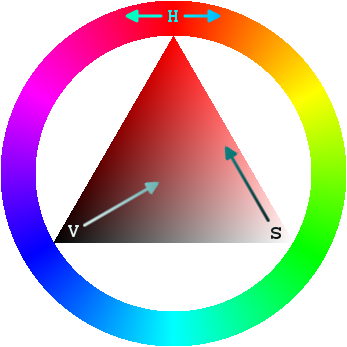
\includegraphics[scale=0.3]{triangulo-HSV.png}
  \end{center}
  \caption{Espacio de color HSV.}
  \label{modelo-RGB}
\end{figure}

\subsection{Uso}

Es común que deseemos elegir un color adecuado para alguna de nuestras aplicaciones, cuando es así resulta muy útil usar la ruleta de color HSV. En ella el matiz se representa por una región circular; una región triangular separada, puede ser usada para representar la saturación y el valor del color. Normalmente, el eje horizontal del triángulo denota la saturación, mientras que el eje vertical corresponde al valor del color. De este modo, un color puede ser elegido al tomar primero el matiz de una región circular, y después seleccionar la saturación y el valor del color deseados de la región triangular.\\

\subsection{Características}

Constituyentes en coordenadas cilíndricas:\\

\subsubsection{Matiz}

Se representa como un grado de ángulo cuyos valores posibles van de 0 a 360$^\circ$ (aunque para algunas aplicaciones se normalizan del 0 al 100 \%). Cada valor corresponde a un color. Ejemplos: 0 es rojo, 60 es amarillo y 120 es verde.
De forma intuitiva se puede realizar la siguiente transformación para conocer los valores básicos RGB:
Disponemos de 360 grados dónde se dividen los 3 colores RGB, eso da un total de 120$^\circ$ por color, sabiendo esto podemos recordar que el 0 es rojo RGB(1, 0, 0), 120 es verde RGB(0, 1, 0) y 240 es azul RGB(0, 0, 1). Para colores mixtos se utilizan los grados intermedios, el amarillo, RGB(1, 1, 0) está entre rojo y verde, por lo tanto 60$^\circ$. Se puede observar como se sigue la secuencia de sumar 60 grados y añadir un 1 o quitar el anterior:\\

\begin{itemize}
\item 0$^\circ$ = RGB(1, 0, 0)
\item 60$^{\circ}$ = RGB(1, 1, 0)
\item 120$^{\circ}$ = RGB(0, 1, 0)
\item 180$^{\circ}$ = RGB(0, 1, 1)
\item 240$^{\circ}$ = RGB(0, 0, 1)
\item 300$^{\circ}$ = RGB(1, 0, 1)
\item 360$^{\circ}$ = 0$^{\circ}$
\end{itemize}

Esta transformación permite saber los tonos de matices que contienen colores puros que contienen toda la cantidad (o ninguna) de los colores R, G y B. Para el color blanco puede poner cualquier matiz y establecer una saturación de 0. Por contra, para el color negro se puede poner cualquier color y saturación, siempre que se ponga un valor de 0.

\subsubsection{Saturación}

Se representa como la distancia al eje de brillo negro-blanco. Los valores posibles van del 0 al 100\%. Dicho parámetro también es conocido como ``pureza''. Cuanto menor sea la saturación de un color, mayor tonalidad grisácea tendrá y más decolorado estará.

\subsubsection{Valor}

El Valor es representativo de la altura en el eje blanco-negro. Los valores posibles varian del 0 al 100\%. 0 se corresponde con el negro. Dependiendo de la saturación, 100 podría ser blanco o un color más o menos saturado.

\subsection{Modelo CYMK}

El modelo CMYK, siendo acrónimo de Cyan, Magenta, Yellow y Key, es un modelo de color ampliamente utilizado en la impresión  de colores. Este modelo permite la representación de una amplia gama de colores y tiene una mejor adaptación a los medios industriales.\\

Este modelo se basa en la mezcla de pigmentos de los siguientes colores para crear otros más:\\

\begin{itemize}
\item C = Cyan (Cian).
\item M = Magenta (Magenta).
\item Y = Yellow (Amarillo).
\item K = Black o Key (Negro).
\end{itemize}

La mezcla de colores CMY ideales en un fondo blanco da como resultado el color negro aunque por diversar razones, el negro generado no es ideal. Por esta razón los dispositivos de impresión a cuatro tintas incorpora la de color negro.\\

\begin{figure}[H]
  \begin{center}
    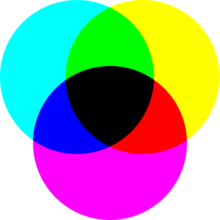
\includegraphics[scale=0.5]{CYMK.png}
  \end{center}
  \caption{Modelo de color CMYK.}
  \label{modelo-RGB}
\end{figure}


% Este archivo es parte de la memoria del proyecto fin de carrera
% de Manuel López Urbina. Protegida bajo la licencia GFDL.
% Para más información, la licencia completa viene incluida en el
% fichero fdl-1.3.tex

% Copyright (C) 2012 Manuel López Urbina

\chapter{Herramientas utilizadas}
\label{chap:herramientas} 

El presente capítulo recoge información acerca de las diferentes herramientas, tanto hardware como software, utilizadas durante el desarrollo del proyecto y para su posterior utilización. 

\section {Herramientas software}

El proyecto ha sido realizado haciendo uso del lenguaje de programación C y C++ junto con el uso de diversas bibliotecas. A continuación se realiza una breve descripción de cada una de ellas:

\begin{description} 

\item [OpenCV]
Es una biblioteca libre de visión artificial originalmente desarrollada por Intel. Desde la salida de su primera versión alfa en el mes de enero de 1999, se ha utilizado en infinidad de aplicaciones. Desde sistemas de seguridad con detección de movimiento, hasta aplicaciones para de control de procesos donde es requerido el reconocimiento de objetos. Esto es debido se publica bajo licencia BSD, permitiendo su utilización para propósitos comerciales y de investigación con las condiciones en ella expresadas.

OpenCV es multiplataforma, existiendo versiones para GNU/Linux, Mac OS X y Windows. Contiene más de 500 funciones que abarcan una gran gama de áreas en el proceso de visión, como reconocimiento de objetos (reconocimiento facial), calibración de cámaras, visión estereo y visión robótica.

El proyecto pretende proporcionar un entorno de desarrollo fácil de utilizar y altamente eficiente. Esto se ha logrado, realizando su programación en código C y C++ optimizados, aprovechando además las capacidades que proveen los procesadores multinúcleo, que como se verá en la presente memoria, su alta eficiencia, ha sido uno de los motivos principales para la elección de esta biblioteca.

\begin{figure}[H]
  \begin{center}
    
\includegraphics[scale=1]{opencv-logo.png}
  \end{center}
  \caption{Logotipo de OpenCV}
  \label{SRV-1}
\end{figure}

\item [Qt] es una biblioteca multiplataforma ampliamente utilizada para el desarrollo de aplicaciones con una interfaz gráfica de usuario, también es usado para el desarrollo de programas sin interfaz gráfica como herramientas para la línea de comandos y consolas para servidores.

Qt utiliza el estándar C++, pero hace un amplio uso de un generador de código especial (llamado compilador Meta Object, o MOC), junto con varias macros para enriquecer el lenguaje. Qt también puede ser usado con otros lenguajes de programación a través de enlaces al lenguaje. Permite su ejecución en las principales plataformas de escritorio y algunas plataformas móviles. También es usado en sistemas informáticos empotrados para automoción, aeronavegación y aparatos domésticos como frigoríficos.

Distribuido bajo los términos de la licencia GNU (entre otras), Qt es software libre y de código abierto. Todas las ediciones soportan el compilador GCC y la suite de Visual Studio entre otros.

\begin{figure}[H]
  \begin{center}
    
\includegraphics[scale=0.3]{qt-logo.jpg}
  \end{center}
  \caption{Logotipo de Qt}
  \label{SRV-1}
\end{figure}

\item [Surveyor Robot Software] software desarrollado por John Cummins junto con los agentes de laboratorio de la Universidad de Brooklyn con la asistencia de M.P. Azhar, y la supervisión del profesor Sklar empleando el lenguaje de programación C++ para el control del vehículo SRV-1 Surveyor. El código está liberado bajo Copyleft.

\item [Simple DirectMedia Layer (SDL)] es un conjunto de bibliotecas desarrolladas en el lenguaje de programación C. Proporciona las funciones básicas para la realización de operaciones de dibujo en dos dimensiones, gestión de efectos de sonido y música, además de carga y gestión de imágenes. Fueron desarrolladas inicialmente por Sam Lantinga, un desarrollador de videojuegos para la plataforma GNU/Linux.

Pese a estar programado en C, tiene wrappers a otros lenguajes de programación como C++, Ada, C\#, BASIC, Erlang, Lua, Java, Python, etc. También proporciona herramientas para el desarrollo de videojuegos y aplicaciones multimedia. Una de sus grandes virtudes es el tratarse de una biblioteca multiplataforma, siendo compatible oficialmente con los sistemas Microsoft Windows, GNU/Linux, Mac OS y QNX, además de otras arquitecturas y sistemas como Sega Dreamcast, GP32, GP2X, etc.
La biblioteca se distribuye bajo la licencia LGPL, que es la que ha provocado el gran avance y evolución de SDL.

\begin{figure}[H]
  \begin{center}
    
\includegraphics[scale=0.3]{sdl-logo.png}
  \end{center}
  \caption{Logotipo de SDL}
  \label{SRV-1}
\end{figure}
\item [Qt Creator] es un IDE creado por Trolltech para el desarrollo de aplicaciones con las bibliotecas Qt.

\begin{figure}[H]
  \begin{center}
    
\includegraphics[scale=0.3]{qtcreator-logo.jpg}
  \end{center}
  \caption{Logotipo de Qt Creator}
  \label{SRV-1}
\end{figure}

\end{description}

\subsection{Licencia}

La aplicación OpenTSR es software libre: usted puede redistribuirlo y / o modificar bajo los términos de la Licencia Pública General de GNU según lo publicado por la Free Software Foundation, ya sea la versión 3 de la Licencia, o (a su elección) cualquier versión posterior.\\

Este programa se distribuye con la esperanza de que sea útil, pero SIN NINGUNA GARANTÍA, incluso sin la garantía implícita de COMERCIALIZACIÓN o IDONEIDAD PARA UN PROPÓSITO PARTICULAR. Ver el GNU General Public License para más detalles. Debería haber recibido una copia de la Licencia Pública General de GNU junto con este documento. Si no es así, consulte \href{http://www.gnu.org/licenses}{GNU Licenses}.

\section{Herramientas hardware}

La figura \ref{figura:elementos-hardware-empleados} nos proporciona una visión general de los diferentes elementos hardware empleados en el desarrollo del proyecto. En los sucesivos puntos se enumeran las características de cada uno de ellos.\\

\begin{figure}[H]
  \begin{center}
    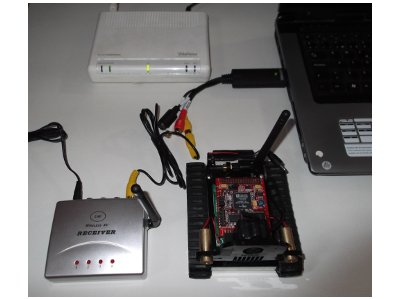
\includegraphics[scale=0.8]{elementos-hardware.jpg}
  \end{center}
  \caption{Imagen de los diferentes elementos hardware empleados.}
  \label{figura:elementos-hardware-empleados}
\end{figure}

\subsection{Vehículo SRV-1}

El elemento hardware principal utilizado es el vehículo \emph{Surveyor SRV-1 WiFi webcam robot}. Dicho vehículo ha sido diseñado para la investigación, la educación, y la exploración, Surveyor SRV-1 es robot que cabe en la palma de la mano, puede desplazarse por superficies lisas y rugosas gracias a sus ruedas tipo tanque fabricadas con caucho. \\

El robot SRV-1 incorpora un potente procesador a 500 MHz denominado Blackfin BF537 con 32 MB de RAM y 4 MB de memoria Flash. Equipado con una cámara a color de resolución 1280x1024 (1,3 megapíxeles) y dos sensores láser que lo dotan de la capacidad de evitar obstáculos. La batería recargable de 7,2 V permite una autonomía de hasta 4 horas de duración y una placa de comunicación WLAN 802.11b/g para su seguimiento y control. \\

\begin{figure}[H]
  \begin{center}
    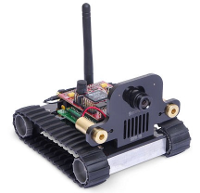
\includegraphics[scale=1]{srv-1.png}
  \end{center}
  \caption{Imagen del vehículo SRV-1}
  \label{SRV-1}
\end{figure}

\subsubsection{Características principales} 

\begin{itemize}
\item Diseño Open Source con acceso completo al código fuente (GPL) y esquemáticos. 
\item El robot es totalmente programable para su funcionamiento autónomo. 
\item Amplio soporte de software a través de aplicaciones de terceros. 
\item Posibilidad de conducir o teleoperar con el robot por medio del software proporcionado (consola java) o de forma remota a través de navegador web. 
\item El software del host es procesado en el servidor web junto con almacenamiento de vídeo en streaming.
\item El robot puede ejecutar programas escritos en C y almacenados en su memoria flash de a bordo. 
\item Control remoto inalámbrico con alcance de 100 metros en interiores y de hasta 1000m en aire libre (visión directa). 
\item El robot puede ser controlado desde un terminal o consola para las pruebas de fácil Linux 2.6 apoyo, así como "bare metal"de programación con GNU BFIN-elf-gcc 
\end{itemize}

\subsubsection{Características hardware} 

\begin{itemize}

\item \textbf{Procesador:} de 500 MHz y 1000 MIPS de nombre Blackfin BF537 con 32MB SDRAM y 4MB de memoria Flash. 

\item \textbf{Cámara:} 1,3 megapíxeles Omnivision OV9655 160x128 resolución de 1280x1024. 

\item \textbf{Placa de control:} Lantronix MatchPort 802.11b/g Wi-Fi 
\item \textbf{Alcance:} 100 metros en interiores, 1000m en situaciones de visión directa. 
\item \textbf{Sensores:} 2 punteros láser para mediciones y soporte para hasta 4 módulos Maxbotics ultrasónicos y varios sensores I2C. 
\item \textbf{Conjunto:} estilo tanque con tracción diferencial a través de cuatro motores reductores de precisión (reducción 100:1). 
\item \textbf{Velocidad:} 20 cm - 40 cm por segundo (aproximadamente 1 pie/seg o 0.5 millas/hora). 
\item \textbf{Chasis:} Aluminio mecanizado. 
\item \textbf{Dimensiones:} 120 mm largo x 100mm ancho x 80mm de altura (5" x 4"x 3"). 
\item \textbf{Peso:} 350gm (12 oz). 
\item \textbf{Potencia:} 7,2 V 2AH Li-poli batería - 4 + horas de autonomía por carga. 
\item \textbf{Cargador:} 100-240VAC 50/60Hz (enchufe de EE.UU.). 1.1.3. 
\end{itemize}

Debido a que el cargador posee el enchufe siguiendo el estándar americano ha sido necesario un conversor a formato europeo para realizar las cargas de la batería que incorpora el vehículo.

\subsubsection{Características software} 

\begin{itemize}

\item \textbf{Firmware del Robot:} fáciles de actualizar, escrito en lenguaje C bajo GPL Open Source, compilado con GNU BFIN-elf-gcc y cadenas de herramientas BFIN-gcc-uClinux. 

\item \textbf{Programación:} el vehículo dispone de un intérprete de lenguaje C con funciones específicas. 

\item \textbf {Comandos de control:} el robot proporciona una serie de comandos para la ejecución de movimientos programables por el usuario desde la memoria Flash de a bordo. 

\item \textbf{Herramientas de desarrollo:} a través de cadenas de herramientas GNU http://blackfin.uclinux.org. 

\item \textbf{Consola del programa:} aplicación basada en Java, funciona en Windows, Mac, Linux. 

\item \textbf {WebcamSat:} módulo de servidor web integrado en el software de la consola, permite que varios espectadores simultáneos remotos a través de Internet. 

\item \textbf{Protocolo de control de robot:} fácil de usar desde otras aplicaciones. 
\end{itemize}

En cuanto a software disponible proporcionado por terceros: 

\begin{itemize}

\item \textbf{RoboRealm:}  SRV-1 puede ser controlado directamente desde RoboRealm, un software basado en Windows con paquete específico para visión artificial en robots. Las extensiones para Robo-Realm SRV-1 permite la creación de guiones que combinan el procesamiento de imágenes de vídeo en vivo desde el robot, por ejemplo, filtrado de color, seguimiento, detección de bordes, extracción de características, y posterior procesamiento de la decisión y movimiento del robot, facilitando la creación de conductas tales como la localización de objetos y el rastreo, evasión de obstáculos, la detección de movimiento, notificación, etc, con una red interfaz, el control puede ser escrito en C / C++, Python, Java, C, Lisp, Visual Basic, WScript y COM a través de la API RoboRealm. 

\item \textbf{Microsoft Robotics Studio:}  Drivers para el SRV-1 de Microsoft Robotics Studio están disponibles. MSRS es un entorno basado en Windows para desarrolladores académicos, aficionados y comerciales para crear aplicaciones de robótica a través de una amplia variedad de hardware. 

\item \textbf{Webots:} Soporte SRV-1 incluido en Webots, es un software de simulación robótica móvil, proporciona un entorno de prototipado rápido para el modelado, la programación y simulación de robots móviles con sistema operativo Windows, Mac / X y Linux. El modelado en 3D y la física son excepcionales. 

\end{itemize}

Para más información acerca del vehículo robótico acceda a la web del \href{http://www.surveyor.com/SRV\_info.html}{sitio oficial}\footnote{Web del sitio oficial: \url{http://www.surveyor.com/SRV\_info.html}.}.

\subsection{Router}

Ha sido necesario disponer de un router para establecer una comunicación inalámbrica entre el ordenador y el vehículo SRV-1. Dicho vehículo posee la característica de realización de conexiones punto a punto o ad-hoc con el inconveniente de ser redes mucho más inestables. \\

Para solucionar el problema de la inestabilidad se ha optado por la creación de una infraestructura de red con la ayuda de un router proporcionando una mayor robustez a la conexión además de permitir incorporar más dispositivos a nuestra red en caso de que sea necesario. \\

\begin{figure}[H]
  \begin{center}
    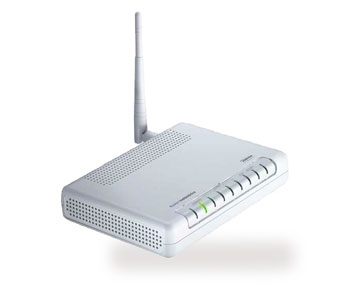
\includegraphics[scale=0.7]{router.png}
  \end{center}
  \caption{Imagen del router empleado.}
  \label{Imagen del router empleado}
\end{figure}

\subsection{Cámara, receptor inalámbrico y capturadora de vídeo}

Para la transmisión de vídeo desde el vehículo al ordenador, debido al estado defectuoso de la cámara incorporada en el vehículo SRV-1, ha sido necesario disponer de una cámara inalámbrica, un receptor inalámbrico para recoger las imágenes de la cámara y una capturadora de vídeo para digitalizarlas y visualizarla en el ordenador.

\subsubsection {Capturadora de vídeo}

El conversor analógico/digital o capturadora empleada es una König modelo CMP-USBVG. Sus características son las siguientes:
 
\begin{itemize}
\item Marca: König.
\item Modelo: CMP-USBVG5.
\item Resolución máxima: 720x480 Píxeles.
\item Sistemas operativos compatibles: Windows 2000/XP/Vista, drivers no oficiales para Linux.
\item Requisitos de energía: 5V.
\item Interfaz:	USB 2.0.
\item Velocidad de captura en vídeo digital: 30 fps.
\item Entrada de S-Video.
\item Entrada compuesta de vídeo.		
\end{itemize}

Consulte la sección \ref{sec:drivers-capturadora} correspondiente a la guía de usuario para acceder a las instrucciones para la instalación de los drivers de la capturadora.\\

\begin{figure}[H]
  \begin{center}
    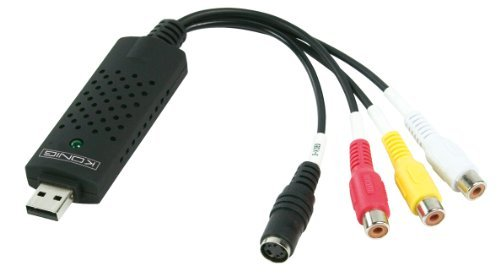
\includegraphics[scale=0.5]{capturadora.jpg}
  \end{center}
  \caption{Imagen de la capturadora o conversor analógico/digital.}
  \label{fig:capturadora}
\end{figure}

\subsubsection{Cámara y receptor inalámbrico} 

La minicámara utilizada está formada por un sensor 1/4'' OmniVision CMOS que ofrece una imagen a color, con una resolución de 380 líneas en TV. Posee un micrófono incorporado que hace que el audio se grabe junto al vídeo. La minicámara es capaz de captar imágenes donde la iluminación es baja siempre y cuando sea superior a 3.0 Lux lo que la hacen adecuada en situaciones de escasa luminosidad. Permite alimentación conectándola directamente a la red  eléctrica o bien usando una pila, gracias al clip de alimentación para pilas de 9V que incorpora.\\

La señal de vídeo y audio se transmite hasta el receptor atravesando paredes y muros. Dispone de una distancia máxima de utilización de 30 metros en situaciones de interior con obstáculos o de hasta 100 metros en exteriores.\\
 
El receptor inalámbrico tiene la posibilidad de recoger la señal de 4 minicámaras gracias a sus cuatro canales, los cuales están capacitados para recoger audio y vídeo por cada canal. Los canales se pueden seleccionar a través de un swich que se encuentra en la parte trasera del receptor. La salida del receptor permite su conexión hacia un videograbador, tarjeta capturadora o monitor mediante un cable RCA. Los canales tiene dos modalidades de visualización y/o grabación, bien mostrando de forma permanente un mismo canal o bien mostrando los cuatro canales de manera secuencial. La alimentación del receptor se hace mediante un alimentador de DC 8V/180 mA.\\

\begin{figure}[H]
  \begin{center}
    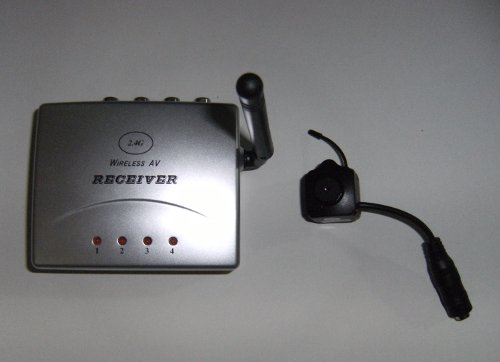
\includegraphics[scale=0.5]{receptor-y-camara.jpg}
  \end{center}
  \caption{Imagen de la cámara y el receptor inalámbricos.}
  \label{imagen-pad}
\end{figure}


\subsection{Gamepad}

Para dotar al vehículo sistema de un control más ergonómico y funcional se ha utilizado un mando con conexión USB como el que muestra la figura \ref{imagen-pad}.\\

\begin{figure}[H]
  \begin{center}
    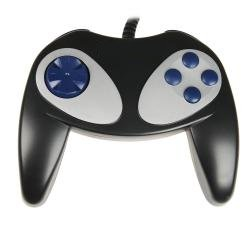
\includegraphics[scale=0.7]{pad.png}
  \end{center}
  \caption{Imagen del gamepad USB utilizado.}
  \label{imagen-pad}
\end{figure}

\subsection{Ordenador}

Por último ha sido necesario un ordenador portátil con un entrono GNU/Linux para la ejecución del software de control, el cual se encargará del procesamiento de las señales de vídeo y la transmisión de las respuestas al vehículo. La aplicación desarrollada también proporciona un medio para el manejo del vehículo por parte del usuario. Imprescindible que el ordenador incorpore de tarjeta WiFi inalámbrica.\\



% Este archivo es parte de la memoria del proyecto fin de carrera
% de Diego Barrios Romero. Protegida bajo la licencia GFDL.
% Para más información, la licencia completa viene incluida en el
% fichero fdl-1.3.tex

% Copyright (C) 2012 Manuel López Urbina

\chapter{Organización temporal}
\label{chap:organización-temporal}

Para el desarrollo de OpenTSR ha sido necesario emplear varias herramientas, utilidades y bibliotecas. Algunas de ellas, ya habían sido utilizadas en ciertas ocasiones a lo largo de la carrera. Sin embargo, otras han requerido un periodo de formación previo, en el que se han adquirido los conocimientos necesarios para poder desarrollar el proyecto.\\

La mayor parte del proceso de investigación fue dedicado al estudio de las diferentes tecnologías existentes para el procesamiento de imágenes. Se comenzó realizando diferentes prototipos funcionales con Matlab, que además de ser un software privativo, no ofrecía la posibilidad de procesamiento de vídeo en tiempo real debido a su escasa velocidad de cálculo.\\

Posteriormente, tras la necesidad de solventar el problema de la velocidad, se optó por elaborar código con la alternativa libre a Matlab, Octave, implementando las funciones críticas en el lenguaje orientado a objetos C++. Resultando también insuficiente.\\

Continuando con las labores de investigación descubrí una biblioteca de uso muy extendido en robótica llamada OpenCV disponible en C, C++ y Python, resultando la disponible en C especialmente rápida en sus cálculos y proporcionando las características deseadas a las necesidades del proyecto, sobre todo la de dotar al sistema de la capacidad cálculo en tiempo real.\\

Todo ello ha implicado un tiempo bastante considerable en el uso, aprendizaje e investigación de las diferentes tecnologías existentes y comprobar su potencial.\\

Una vez decidida la herramienta para el procesamiento de imágenes, se consideró necesaria la idea de implementar una interfaz acorde con el sistema que permita el visionado de resultados al usuario y el entorno por el que se desplaza el vehículo. Para ello se utilizó la biblioteca Qt escrita en C++. Por tanto fue necesario tiempo para adquirir las nociones básicas de la biblioteca con la ayuda del entorno de desarrollo QtCreator.\\

Por otro lado, existen multitud de algoritmos y técnicas propias del reconocimiento de patrones que no son estudiadas durante la Ingeniería Técnica en Informática y que sí son vistas en la Ingeniería Informática añadiendo la necesidad de estudios de los conceptos propios del reconocimiento de patrones. Todo ello me ha supuesto un esfuerzo de investigación y aprendizaje bastante considerable.\\

Una vez determinadas las diferentes herramientas a utilizar se comenzó con la implementación de los diferentes prototipos funcionales para el software de reconocimiento de imágenes. Finalizado el software de reconocimiento se elaboró el sistema de comunicaciones con el vehículo y la interfaz gráfica.\\

La figura \ref{gantt:tareas} muestra una visión de las diferentes tareas desarrolladas para la elaboración del proyecto junto con la descomposición de cada una de ellas:\\

\begin{figure}[H]
  \begin{center}
    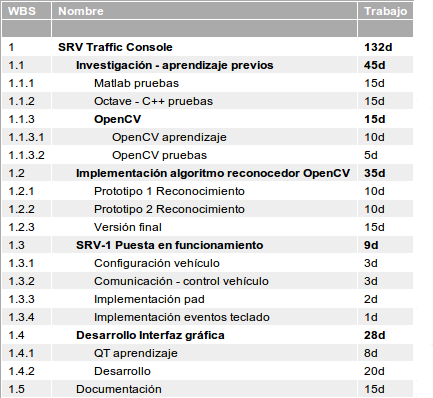
\includegraphics[scale=1]{tareas-gantt.png}
  \end{center}
  \caption{Descomposición de las tareas implicadas en el desarrollo del proyecto.}
  \label{gantt:tareas}
\end{figure}


\figura{gantt-1.png}{scale=0.5}{Diagrama de Gantt 1. Desarrollo del
  proyecto.}{gannt}{H}

\figura{gantt-2.png}{scale=0.5}{Diagrama de Gantt 2. Desarrollo del
  proyecto.}{gannt-2.png}{H}

\figura{gantt-3.png}{scale=0.5}{Diagrama de Gantt 3. Desarrollo del
  proyecto.}{gannt-3.png}{H}


% Este archivo es parte de la memoria del proyecto fin de carrera
% de Diego Barrios Romero. Protegida bajo la licencia GFDL.
% Para más información, la licencia completa viene incluida en el
% fichero fdl-1.3.tex

% Copyright (C) 2012 Manuel López Urbina

\chapter{Montaje hardware}
\label{chap:dispositivos-hardware}

\section{Colocación de la cámara en el vehículo}

Para la obtención de la imágenes se ha elegido una pequeña cámara inalámbrica con el fin de no limitar la capacidad de movimiento del vehículo.\\

 La cámara ha sido situada en la parte delantera del vehículo en el soporte que dispone para la colocación de la misma. Destacar que se ha empleado el sistema de cámara independiente debido al estado defectuoso de la cámara original del vehículo.\\

Para la alimentación de la cámara se ha añadido una pila de 9 voltios en la parte trasera del vehículo. En la imagen \ref{fig:coche-camara-pila} se puede visualizar el conjunto vehículo, cámara y pila de alimentación montados.\\

\begin{figure}[H]
  \begin{center}
    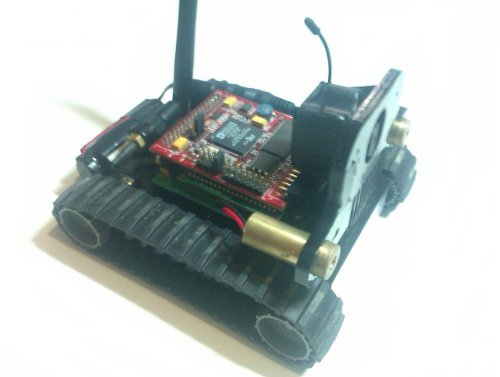
\includegraphics[scale=0.5]{coche-camara-pila.jpg}
  \end{center}
  \caption{Vehículo SRV-1 tras el montaje de la cámara.}
  \label{fig:coche-camara-pila}
\end{figure}


\section{Conexión cámara - PC}

Para conectar la cámara al ordenador, al tratarse de una cámara inalámbrica, resulta necesario utilizar un receptor. Las imágenes son trasmitidas mediante radiofrecuencia desde la cámara al sistema receptor que se encuentra conectado al PC mediante una capturadora de vídeo USB.\\

El sistema receptor de vídeo consiste en un capturador de imágenes analógico que recibe imágenes analógicas a través de radiofrecuencia. El receptor, posteriormente, a través de conectores RCA envía la imagen analógica al conversor analógico/digital convirtiendo la imagen analógica en imagen digital con una resolución de 720x576 píxeles, y que a su vez se encuentra conectado al PC mediante un cable USB, éste último dispositivo es también conocido como capturadora de vídeo.\\

El ordenador detecta la cámara como si de una webcam se tratara. El funcionamiento del sistema receptor se esquematiza en la figura \ref{esquema-sistema-receptor-video}. Indicar que el receptor de imagen analógico se alimenta con un adaptador de corriente. \\

\begin{figure}[H]
  \begin{center}
    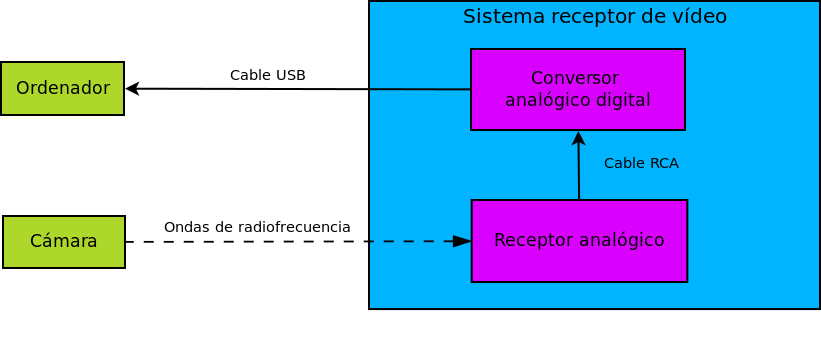
\includegraphics[scale=0.5]{esquema-sistema-receptor-video.png}
  \end{center}
  \caption{Esquema del sistema de recepción de imágenes desde la cámara al ordenador.}
  \label{esquema-sistema-receptor-video}
\end{figure}

En la figura \ref{fig:conjunto-video} se muestra una fotografía del conjunto correctamente conectado:\\

\begin{figure}[H]
  \begin{center}
    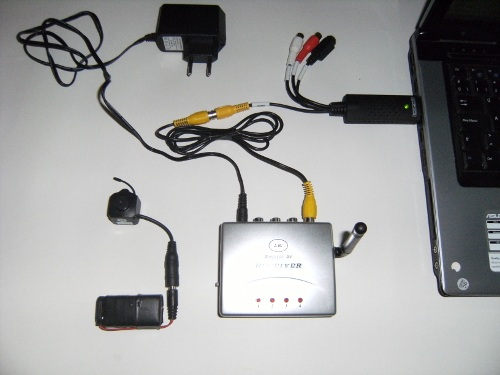
\includegraphics[scale=0.7]{conjunto-video.jpg}
  \end{center}
  \caption{Visión del sistema de recepción de imágenes montado a falta de la conexión a corriente del receptor.}
  \label{fig:conjunto-video}
\end{figure}


\section{Comunicaciones vehículo - PC}

Para establecer las comunicaciones entre el vehículo robótico y el ordenador ha sido necesario disponer de un router Wi-Fi para la creación de una infraestructura de red, de tal manera que, el vehículo SRV-1 realice automáticamente una conexión al router tras activarse el interruptor de encendido. Por otra parte, el ordenador deberá de conectarse al router como de si una red convencional se tratara. Se ha optado por este sistema debido a que presenta una mayor estabilidad que realizar una conexión directa ad hoc entre el ordenador y el vehículo.\\

En la sección \ref{sec:configuración-router} del manual de usuario se detalla el proceso de configuración del router Xavi 7868r utilizado.\\

El vehículo debe ser configurado según los valores previamente fijados en el router de tal manera que cuando el vehículo sea puesto en marcha realice una conexión de manera automática e inalámbrica con el router integrándose en la red. En el manual de usuario, sección \ref{sec:configuración-srv}, se detalla los pasos y parámetros necesarios para su correcta configuración.\\


La figura \ref{fig:com-coche-pc} de a continuación muestra un esquema de las comunicaciones entre el vehículo y el ordenador mediante el uso de un router.\\

\begin{figure}[H]
  \begin{center}
    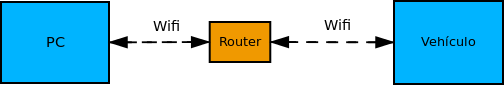
\includegraphics[scale=0.8]{comunicacion-coche-robot.png}
  \end{center}
  \caption{Comunicaciones vía Wi-Fi entre el ordenador y el vehículo robótico mediante un router.}
  \label{fig:com-coche-pc}
\end{figure}


\begin{figure}[H]
  \begin{center}
    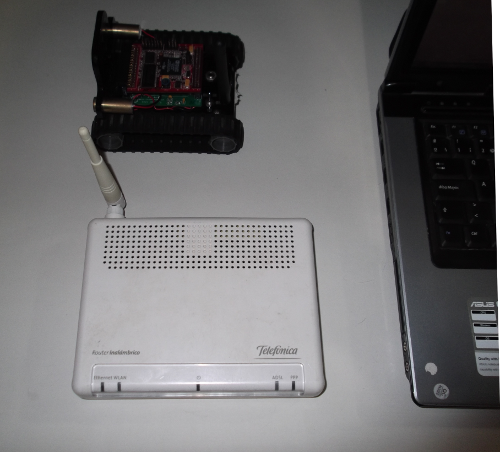
\includegraphics[scale=0.6]{sistema-comunicaciones-coche-pc.png}
  \end{center}
  \caption{Vista del sistema de comunicaciones entre el vehículo y el ordenador.}
  \label{fig:conjunto-video}
\end{figure}



% Este archivo es parte de la memoria del proyecto fin de carrera
% de Manuel López Urbina. Protegida bajo la licencia GFDL.
% Para más información, la licencia completa viene incluida en el
% fichero fdl-1.3.tex

% Copyright (C) 2012 Manuel López Urbina

\chapter{Desarrollo software}
\label{chap:desarrollo-software}

\section{Metodología de desarrollo}

Este proyecto ha sido obtenido empleando una metodología de desarrollo basada en el modelo de construcción de prototipos para la parte software referente a la visión artificial y una metodología de desarrollo en cascada para el desarrollo de la interfaz gráfica y software de control del vehículo.\\

El modelo de construcción de prototipos proporciona una serie de características que lo hacen idóneo para este proyecto. Dicho modelo resulta especialmente útil en las siguientes situaciones:

\begin{itemize}
\item El cliente define los objetivos generales del software sin entrar en detalles pormenorizados de los requisitos de entrada, procesamiento o salida a obtener.
\item El responsable del desarrollo del software desconoce demasiados aspectos del desarrollo tales como, eficacia de un determinado algoritmo, capacidad de adaptación de un sistema operativo, definición de la interacción hombre-máquina entre otros.
\end{itemize}

Por otro lado, el modelo de desarrollo en cascada resulta adecuado para las siguientes situaciones:

\begin{itemize}
\item Se dispone de unos requisitos claros y precisos.
\item El sistema a desarrollar es de pequeña envergadura.
\item Las tecnologías utilizadas son conocidas por los desarrolladores.
\end{itemize}

Centrándonos nuevamente en el desarrollo del proyecto, los motivos que llevaron a cabo la elección del modelo de desarrollo por prototipos para la obtención del software de visión artificial fueron el amplio desconocimiento existente en cuanto a los algoritmos existentes y su eficacia e idoneidad al producto deseado. \\

En cambio, para el desarrollo de la interfaz gráfica y software de control del vehículo, se optó por el seguimiento del modelo de desarrollo en cascada al tratarse de un desarrollo con una menor dificultad técnica y la disponibilidad de los requisitos necesarios.\\

Por tanto el proyecto queda distribuido en tres subsistemas:

\begin{itemize}
\item Subsistema de visión artificial.
\item Subsistema de control.
\item Subsistema gráfico.
\end{itemize}


\begin{figure}[H]
  \begin{center}
    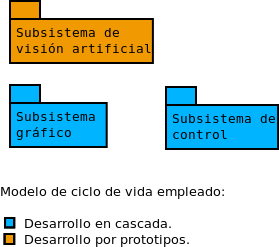
\includegraphics[scale=1]{subsistemas.png}
  \end{center}
  \caption{Subsistemas existentes en el proyecto junto con el modelo de ciclo de vida utilizado para su desarrollo.}
  \label{subsistemas}
\end{figure}

\section{Recolección de requisitos}

\subsection{Requisitos funcionales}

Para la elaboración de este proyecto se ha utilizado la metodología Métrica V3 así como el estándar ISO/IEC 12207. Métrica es una metodología de planificación, desarrollo y mantenimiento de los sistemas de información desarrollada por el Ministerio de Administraciones Públicas del Gobierno de España. Tiene como objetivo proporcionar una guía para la sistematización de actividades del ciclo de vida de los proyectos software en el ámbito de las administraciones públicas.\\

Métrica V3\cite{website:metrica} está basada en el modelo de procesos del ciclo de vida de desarrollo ISO/IEC 12207 (Information Technology - Software Life Cycle Processes) así como en la norma ISO/IEC 15504 SPICE (Software Process Improvement And Assurance Standards Capability Determination).\\

En la página oficial de Métrica V3, sus desarrolladores indican que puede ser utilizada libremente con la única restricción de citar la fuente de su propiedad intelectual, la del Ministerio de Administraciones Públicas.\\

Un caso de uso es una descripción de los pasos o actividades que deberán realizarse para llevar a cabo algún proceso. Los objetivos de los casos de uso son los siguientes:

\begin{itemize}
\item Obtener los requisitos funcionales del sistema y expresarlos desde un punto de vista más cercano al usuario.
\item Proporcionar una guía de todo el proceso de desarrollo del sistema de información. Los casos de uso proporcionan, por tanto, un modo claro y preciso de comunicación entre lo que desea el cliente y el desarrollador proporcionando desde el punto de vista del cliente una visión de ``caja negra'' del sistema eliminando los detalles de su construcción o desarrollo. Para los desarrolladores es utilizado como punto de partida y el eje sobre el que se apoya todo el desarrollo del sistema en los procesos de análisis y diseño.
\end{itemize}

Los requisitos funcionales que se han obtenido después del proceso de obtención de requisitos son los siguientes:

\begin{itemize}
\item Conectar con vehículo.
\item Desconectar con vehículo.
\item Pilotaje tradicional.
\item Pilotaje autónomo
\end{itemize}

\subsection{Diagramas de casos de uso}
\label{sec:casos-de-uso}

Los diagramas de caso de uso muestra una representación del comportamiento ofrecido por el sistema de información desde el punto de vista del usuario. El comportamiento del sistema es representado como un conjunto de transacciones ejecutadas entre el sistema y los actores junto con la descripción sobre las de las relaciones de comunicación existentes entre un actor y el sistema.\\

En la figura \ref{caso-de-uso} podemos observar el diagrama de casos de uso resultante tras la recolección de requisitos:\\

\begin{figure}[H]
  \begin{center}
    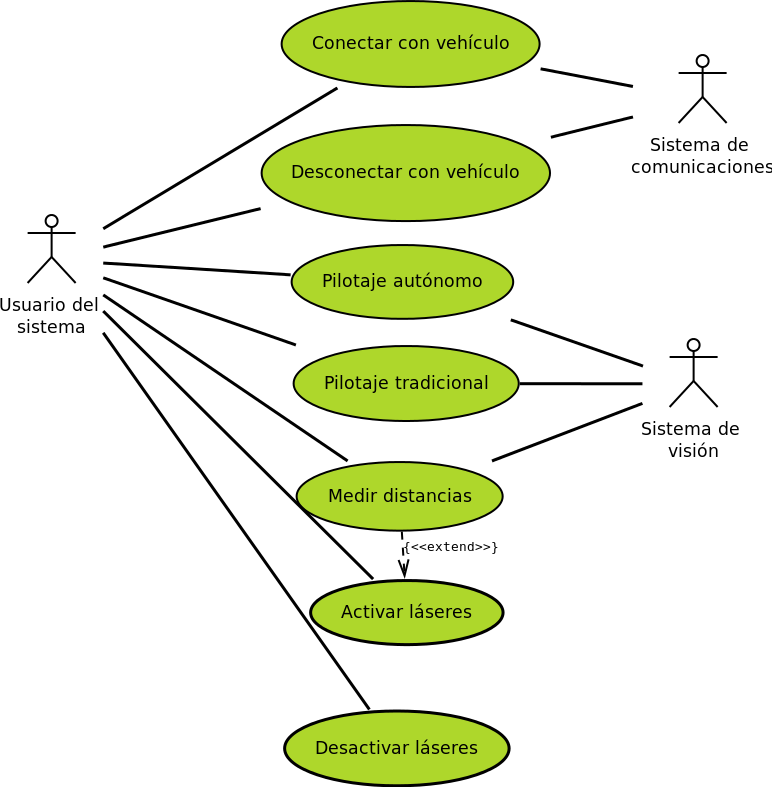
\includegraphics[scale=0.5]{diagrama-caso-de-uso.png}
  \end{center}
  \caption{Diagrama de casos de uso.}
  \label{caso-de-uso}
\end{figure}

\subsection{Especificación de los casos de uso}

A continuación se proporciona la especificaciones de cada uno de los casos de uso de la sección \ref{sec:casos-de-uso}.\\

\begin{table}[H]
  \begin{center}
    \begin{tabular}{|p{3.5cm}|p{10cm}|}
      \hline
      {\textbf{Caso de uso:}} & { Conexión coche.} \\
      \hline
      {\textbf{Descripción:}} & {El sistema deberá conectarse como describe el presente caso de uso cuando el operador del sistema desee conectar con el vehículo.} \\
     \hline
     \multicolumn{2}{c}{\emph{continua en la siguiente página ...}}\\
    \end{tabular}
  \end{center}
\end{table}    

\begin{table}[H]
  \begin{center}
    \begin{tabular}{|p{3.5cm}|p{10cm}|}
     \multicolumn{2}{c}{\emph{continua de la página anterior...}}\\
     \hline
      {\textbf{Actor principal:}} & { Operador del sistema.} \\
      \hline
      {\textbf{Actor secundario:}} & { Sistema de comunicaciones.} \\
     \hline
      {\textbf{Precondiciones:}} & { El sistema de comunicaciones deberá estar libre.} \\
     \hline     
     {\textbf{Flujo principal:}} & { 
\begin{enumerate}
\item El actor operador del sistema solicita establecer conexión con el coche.
\item El sistema comprueba que se puede establecer comunicación.
\item El sistema establece una conexión entre el ordenador personal y el coche mostrando por pantalla que la conexión se ha realizado exitosamente.
\end{enumerate}} \\
\hline
     {\textbf{Postcondición:}} & {Se establece una conexión entre el ordenador personal y el coche.}\\
     \hline
     {\textbf{Excepciones:}} & {Si no se encuentra el vehículo el sistema indicará error.}\\
     \hline
    \end{tabular}
  \end{center}
\caption{Descripción de caso de uso: Conexión coche.}
\end{table}


\begin{table}[H]
  \begin{center}
    \begin{tabular}{|p{3.5cm}|p{10cm}|}
      \hline
      {\textbf{Caso de uso:}} & { Desconexión del vehículo.} \\
      \hline
      {\textbf{Descripción:}} & { El sistema deberá actuar como describe en este caso de uso cuando el operador del sistema solicita la desconexión con el vehículo.} \\
     \hline
      {\textbf{Actor principal:}} & { Operador del sistema.} \\
      \hline
      {\textbf{Actor secundario:}} & { sistema de comunicaciones.} \\
      \hline
      {\textbf{Precondiciones:}} & { El sistema de comunicaciones deberá estar ocupado con una conexión activa.} \\
     \hline   
    {\textbf{Flujo principal:}} & { 
      \begin{enumerate}
\item El actor operador del sistema solicita la desconexión con el vehículo.
\item El sistema comprueba que se encuentra establecida una conexión entre el ordenador y el coche.
\item El sistema finaliza la conexión entre el ordenador y el vehículo e indica por pantalla que la desconexión se ha realizado con éxito.
\end{enumerate}
} \\
     \hline
     {\textbf{Postcondición}} & {Se finaliza la conexión entre el ordenador y el vehículo.}\\
     \hline
         {\textbf{Excepciones:}} & {No existe conexión entre el equipo y el vehículo.}\\
         \hline
    \end{tabular}
  \end{center}
\caption{Descripción del caso de uso: Desconexión coche.}
\end{table}

\begin{table}[H]
  \begin{center}
    \begin{tabular}{|p{3.5cm}|p{10cm}|}
      \hline
      {\textbf{Caso de uso:}} & { Pilotaje tradicional.} \\
      \hline
      {\textbf{Descripción:}} & {El sistema deberá comportarse como describe el presente caso de uso cuando el operador del sistema decida comenzar con el pilotaje tradicional del vehículo.} \\
     \hline
      {\textbf{Actor principal:}} & { Operador del sistema.} \\
      \hline
      {\textbf{Actor secundario:}} & {Sistema de visión artificial}\\
      \hline
      {\textbf{Precondiciones:}} & { Se encuentra establecida una conexión entre el ordenador y el vehículo y se están procesando imágenes.} \\
     \hline     
     {\textbf{Flujo principal:}} & { 
       \begin{enumerate}
       \item El actor operador del sistema solicita el pilotaje tradicional del vehículo.
       \item El sistema comprueba que existe una conexión activa entre el ordenador y el vehículo, y también que se están
         procesando imágenes.
       \item El sistema muestra las señales de tráfico detectadas en un momento determinado.
       \end{enumerate}
     } \\
     \hline
     {\textbf{Postcondición:}} & {Se comienza a pilotar el vehículo visualizándose las señales de tráfico del entorno.}\\
     \hline
     {\textbf{Excepciones:}} & {Si no se encuentra establecida la conexión entre el vehículo y el ordenador informa del error.}\\        
     \hline
    \end{tabular}
  \end{center}
\caption{Descripción del caso de uso: Pilotaje tradicional.}
\end{table}


\begin{table}[H]
  \begin{center}
    \begin{tabular}{|p{3.5cm}|p{10cm}|}
      \hline
      {\textbf{Caso de uso:}} & { Pilotaje autónomo.} \\
      \hline
      {\textbf{Descripción:}} & {El sistema deberá comportarse como describe el presente caso de uso cuando el operador del sistema decida comenzar con el pilotaje autónomo del vehículo.} \\
     \hline
      {\textbf{Actor principal:}} & { Operador del sistema.} \\
      \hline
      {\textbf{Actor secundario:}} & {Sistema de visión artificial}\\
      \hline
      {\textbf{Precondiciones:}} & { Se encuentra establecida una conexión entre el ordenador y el vehículo y se están procesando imágenes.} \\
     \hline 
    \multicolumn{2}{c}{\emph{continua en la siguiente página ...}}\\
    \end{tabular}
  \end{center}
\end{table}

\begin{table}[H]
  \begin{center}
    \begin{tabular}{|p{3.5cm}|p{10cm}|}
     \multicolumn{2}{c}{\emph{continua de la página anterior...}}\\
      \hline
     {\textbf{Flujo principal:}} & { 
       \begin{enumerate}
       \item El actor operador del sistema solicita el pilotaje autónomo del vehículo.
       \item El sistema comprueba que existe una conexión activa entre el ordenador y el vehículo, y también que se están
         procesando imágenes.
       \item El sistema muestra las señales de tráfico detectadas en un momento determinado.
       \item El vehículo realiza la operación correspondiente a la señal detectada.
       \end{enumerate}
     } \\
     \hline
     {\textbf{Postcondición:}} & {Se comienza a pilotar el vehículo visualizándose las señales de tráfico del entorno.}\\
     \hline
     {\textbf{Excepciones:}} & {Si no se encuentra establecida la conexión entre el vehículo y el ordenador informa del error.}\\        
     \hline
    \end{tabular}
  \end{center}
\caption{Descripción del caso de uso: Pilotaje autónomo.}
\end{table}


\begin{table}[H]
  \begin{center}
    \begin{tabular}{|p{3.5cm}|p{10cm}|}
      \hline
      {\textbf{Caso de uso:}} & { Medir distancias.} \\
      \hline
      {\textbf{Descripción:}} & {El sistema deberá mostrar la distancia a la que se encuentra un obstáculo del vehículo utilizando sus punteros láser.} \\
     \hline
      {\textbf{Actor principal:}} & { Operador del sistema.} \\
      \hline
      {\textbf{Actor secundario:}} & {Sistema de visión artificial}\\
      \hline
      {\textbf{Precondiciones:}} & { Se encuentra establecida una conexión entre el ordenador y el vehículo y se están procesando imágenes.} \\
     \hline 
     \multicolumn{2}{c}{\emph{continua en la siguiente página ...}}\\
    \end{tabular}
  \end{center}
\end{table}    

\begin{table}[H]
  \begin{center}
    \begin{tabular}{|p{3.5cm}|p{10cm}|}
     \multicolumn{2}{c}{\emph{continua de la página anterior...}}\\
     \hline
     {\textbf{Flujo principal:}} & { 
       \begin{enumerate}
       \item El actor operador del sistema solicita la medición de distancias.
       \item El sistema comprueba que existe una conexión activa entre el ordenador y el vehículo, y también que se están
         procesando imágenes.
       \item El sistema comprueba que se encuentran los láseres activados.
       \item El sistema calcula la distancia a partir de los puntos del láser reflejados en la imagen captada.
       \item Los punteros láser no se encuentran activados: extend activar láseres.
       \item El sistema muestra la distancia real en centímetros entre el vehículo y el obstáculo.
       \end{enumerate}
     } \\
     \hline
     {\textbf{Postcondición:}} & { El sistema muestra la distancia real en centímetros entre el vehículo y el obstáculo frontal.}\\
     \hline
     {\textbf{Excepciones:}} & {Si no se encuentra establecida la conexión entre el vehículo y el ordenador informa del error.}\\        
     \hline
    \end{tabular}
  \end{center}
\caption{Descripción del caso de uso: Medir distancias.}
\end{table}


\begin{table}[H]
  \begin{center}
    \begin{tabular}{|p{3.5cm}|p{10cm}|}
      \hline
      {\textbf{Caso de uso:}} & { Activar láseres.} \\
      \hline
      {\textbf{Descripción:}} & {El vehículo deberá activar los punteros láser.} \\
     \hline
      {\textbf{Actor principal:}} & { Operador del sistema.} \\
      \hline
      {\textbf{Actor secundario:}} & {}\\
      \hline
      {\textbf{Precondiciones:}} & { Se encuentra establecida una conexión entre el ordenador.} \\
     \hline 
     {\textbf{Flujo principal:}} & { 
       \begin{enumerate}
       \item El actor operador del sistema solicita la activación de los punteros láser.
       \item El sistema comprueba que existe una conexión activa entre el ordenador y el vehículo.
       \item El sistema comprueba que se encuentran los láseres desactivados.
       \item El sistema activa los láseres.
       \end{enumerate}
     } \\
     \hline
     {\textbf{Postcondición:}} & { El vehículo activa los punteros láser.}\\
     \hline
     {\textbf{Excepciones:}} & {Si no se encuentra establecida la conexión entre el vehículo y el ordenador se informa del error.}\\        
     \hline
    \end{tabular}
  \end{center}
\caption{Descripción del caso de uso: Activar láseres.}
\end{table}


\begin{table}[H]
  \begin{center}
    \begin{tabular}{|p{3.5cm}|p{10cm}|}
      \hline
      {\textbf{Caso de uso:}} & { Desactivar láseres.} \\
      \hline
      {\textbf{Descripción:}} & {El vehículo deberá desactivar los punteros láser.} \\
     \hline
      {\textbf{Actor principal:}} & { Operador del sistema.} \\
      \hline
      {\textbf{Actor secundario:}} & {}\\
      \hline
      {\textbf{Precondiciones:}} & { Se encuentra establecida una conexión entre el ordenador.} \\
     \hline 
     {\textbf{Flujo principal:}} & { 
       \begin{enumerate}
       \item El actor operador del sistema solicita la desactivación de los punteros láser.
       \item El sistema comprueba que existe una conexión activa entre el ordenador y el vehículo.
       \item El sistema comprueba que se encuentran los láseres activados.
       \item El sistema desactiva los láseres.
       \end{enumerate}
     } \\
     \hline
     \multicolumn{2}{c}{\emph{continua en la siguiente página ...}}\\
    \end{tabular}
  \end{center}
\end{table}    

\begin{table}[H]
  \begin{center}
    \begin{tabular}{|p{3.5cm}|p{10cm}|}
     \multicolumn{2}{c}{\emph{continua de la página anterior...}}\\
     \hline
     {\textbf{Postcondición:}} & { El vehículo desactiva los punteros láser.}\\
     \hline
     {\textbf{Excepciones:}} & {Si no se encuentra establecida la conexión entre el vehículo y el ordenador se informa del error.}\\        
     \hline
    \end{tabular}
  \end{center}
\caption{Descripción del caso de uso: Desactivar láseres.}
\end{table}





\subsection{Desarrollo}

La elaboración de los diferentes prototipos del software de visión artificial junto con la obtención del software de comunicación y la interfaz gráfica queda recogido al detalle en los sucesivos temas.\\

La distribución es la siguiente:

\begin{itemize}
\item El capítulo \ref{chap:reconocimiento} se describen cada uno de los prototipos desarrollados para el software de visión artificial. 
\item El capítulo \ref{chap:software-de-control} se centra en el desarrollo de la comunicación con el vehículo. 
\item El capítulo \ref{chap:interfaz-gráfica} abarca el desarrollo de la interfaz gráfica.
\end{itemize}




% Este archivo es parte de la memoria del proyecto fin de carrera
% de Manuel López Urbina. Protegida bajo la licencia GFDL.
% Para más información, la licencia completa viene incluida en el
% fichero fdl-1.3.tex

% Copyright (C) 2012 Manuel López Urbina

\chapter{Software de reconocimiento}
\label{chap:reconocimiento}

Una vez descritos los diferentes elementos hardware utilizados y la metodología de desarrollo empleada, en el presente capítulo  sucesivos se realizará un profundo análisis de las técnicas y problemas detectados durante el desarrollo, comenzando en el presente tema por el software de reconocimiento. Este subsistema ha sido elaborado siguiendo el modelo de construcción por prototipos.\\

A modo introductorio, destacar que el software de reconocimiento ha sido elaborado haciendo uso de la biblioteca OpenCV para el lenguaje C. Esta biblioteca incluye los elementos necesarios para el tratamiento de imágenes para, como se ha descrito en la sección \ref{sec:objetivos} de objetivos, proporcionar al vehículo de un sistema de reconocimiento de señales de tráfico.\\

Las señales de tráfico detectables por el sistema serán las siguientes:\\

\begin{figure}[H]
  \begin{center}
    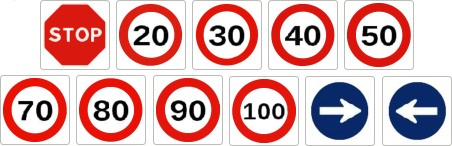
\includegraphics[scale=1]{seniales2.png}
  \end{center}
  \caption{Conjunto de señales de tráfico detectables por el sistema.}
  \label{conjunto-señales-rp}
\end{figure}

Entre las señales incluidas disponemos las diferentes señales indicadoras de velocidad máxima, existiendo desde la de 20 km/h hasta la de 100 km/h con el objetivo de poder ajustar automáticamente la velocidad del vehículo en función de la señal detectada.\\

Por otro lado existen las señales indicadoras de dirección obligatoria, con el fin de efectuar giros y la señal de stop con el propósito de efectuar paradas de manera automática.\\

Para la elaboración del sistema ha sido necesario el desarrollo de tres prototipos. En las sucesivas secciones del tema se describirán cada uno de los ellos junto con los problemas detectados y motivos por los que finalmente se acabaron desechando junto con las soluciones adoptadas.

\section {Primer prototipo}

Para el desarrollo del primer prototipo se han empleado las siguientes técnicas:

\begin{enumerate}
\item Segmentación por color de la imagen de entrada.
\item Eliminación de objetos pequeños resultantes con área inferior a un determinado valor.
\item Extracción de la imagen de objetos existentes.
\item Comparación de cada uno de los objetos con plantillas para su identificación.
\end{enumerate}

\subsection{Obtención de la imagen}

El paso previo de todo sistema de reconocimiento de objetos es la extracción de características a partir de unos datos de entrada para su posterior análisis. La información de entrada es proporcionada al sistema mediante una imagen, la cual es obtenida a través de la cámara que dota el vehículo.\\

Sin embargo, lo único que se recibe es una matriz de números desde la cámara.\\

\begin{figure}[H]
  \begin{center}
    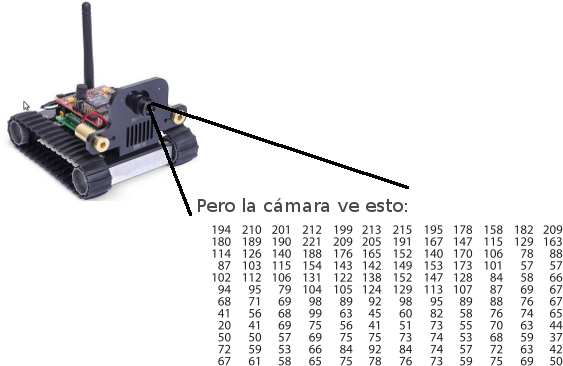
\includegraphics[scale=0.5]{datos-camara.png}
  \end{center}
  \caption{Interpretación de una imagen por parte de una cámara}
  \label{imagen-entrada-rp}
\end{figure}

Dicha matriz de números es recibida por el ordenador para su posterior interpretación y tratamiento\footnote{El procedimiento empleado para la transmisión de la imagen desde el vehículo al computador de manera física queda reflejado en el tema \ref{chap:dispositivos-hardware} correspondiente al montaje de los dispositivos hardware.}. \\

A continuación se muestra el código realizado en OpenCV para la obtención de las imágenes a partir de una cámara:\\

\underline{Algoritmo de obtención de imágenes}\\
\begin{Verbatim}[commandchars=\\\{\}]
\PY{c+cp}{#}\PY{c+cp}{include <stdio.h>}
\PY{c+cp}{#}\PY{c+cp}{include <stdlib.h>}
\PY{c+cp}{#}\PY{c+cp}{include "opencv}\PY{c+cp}{/}\PY{c+cp}{cv.h" }
\PY{c+cp}{#}\PY{c+cp}{include "opencv}\PY{c+cp}{/}\PY{c+cp}{highgui.h"}

\PY{k+kt}{int} \PY{n+nf}{main}\PY{p}{(}\PY{k+kt}{int} \PY{n}{argc}\PY{p}{,} \PY{k+kt}{char} \PY{o}{*}\PY{n}{argv}\PY{p}{[}\PY{p}{]}\PY{p}{)}
\PY{p}{\PYZob{}}
  \PY{n}{IplImage} \PY{o}{*}\PY{n}{img}\PY{o}{=}\PY{n+nb}{NULL}\PY{p}{;}

  \PY{k+kt}{char} \PY{n}{c}\PY{o}{=}\PY{n+nb}{NULL}\PY{p}{;}

  \PY{c+c1}{// Crea una ventana llamada Imagen}
  \PY{c+c1}{// con tamaño predeterminado.}
  \PY{n}{cvNamedWindow}\PY{p}{(}\PY{l+s}{"}\PY{l+s}{Imagen}\PY{l+s}{"}\PY{p}{,}\PY{n}{CV\PYZus{}WINDOW\PYZus{}AUTOSIZE}\PY{p}{)}\PY{p}{;}
 
  \PY{c+c1}{// Crea la conexion con la Webcam.}
  \PY{n}{CvCapture}\PY{o}{*} \PY{n}{captura} \PY{o}{=} \PY{n}{cvCaptureFromCAM}\PY{p}{(}\PY{o}{-}\PY{l+m+mi}{1}\PY{p}{)}\PY{p}{;}
 
   \PY{c+c1}{// Si la tecla pulsada es ESC se sale del bucle.}
   \PY{k}{while}\PY{p}{(}\PY{n}{c} \PY{o}{!}\PY{o}{=} \PY{l+m+mi}{27}\PY{p}{)} \PY{p}{\PYZob{}} 

    \PY{c+c1}{// Añade el frame capturado dentro de la imagen img.}
    \PY{n}{img} \PY{o}{=} \PY{n}{cvQueryFrame}\PY{p}{(}\PY{n}{captura}\PY{p}{)}\PY{p}{;}

    \PY{c+c1}{// PROCESAMIENTO DE LA IMAGEN.}
  
    \PY{c+c1}{// Se espera la pulsación de alguna tecla }
    \PY{c+c1}{// durante 10 milésimas de segundo.}
    \PY{c+c1}{// De ser alguna tecla pulsada, }
    \PY{c+c1}{// se almacena en la variable c.}
    \PY{n}{c} \PY{o}{=} \PY{n}{cvWaitKey}\PY{p}{(}\PY{l+m+mi}{10}\PY{p}{)}\PY{p}{;}
  \PY{p}{\PYZcb{}}

  \PY{c+c1}{// Liberación de la cámara.}
  \PY{n}{cvReleaseCapture}\PY{p}{(}\PY{o}{&}\PY{n}{captura}\PY{p}{)}\PY{p}{;}

  \PY{c+c1}{// Eliminamos todas las estructuras ventana existentes. }
  \PY{n}{cvDestroyAllWindows}\PY{p}{(}\PY{p}{)}\PY{p}{;} 
   
  \PY{k}{return} \PY{l+m+mi}{0}\PY{p}{;}
\PY{p}{\PYZcb{}}
\end{Verbatim}


Una vez obtenida la imagen, ésta es almacenada en la variable, \emph{img} del código anterior. A partir de ese instante se dispone de la base para aplicar la extracción de características y el procesamiento de la imagen que se desee aplicar añadiendo el código necesario en la parte interna del bucle del código mostrado. Una vez finalizado el procesamiento aplicado a la imagen capturada se obtiene un nuevo frame para continuar con el procesamiento de una nueva imagen mientras la tecla ESC no sea presionada.\\

Un ejemplo de una imagen de entrada capturada por la cámara y visionada en la pantalla del ordenador utilizando el código anteriormente mostrado puede ser el siguiente:\\

\begin{figure}[H]
  \begin{center}
    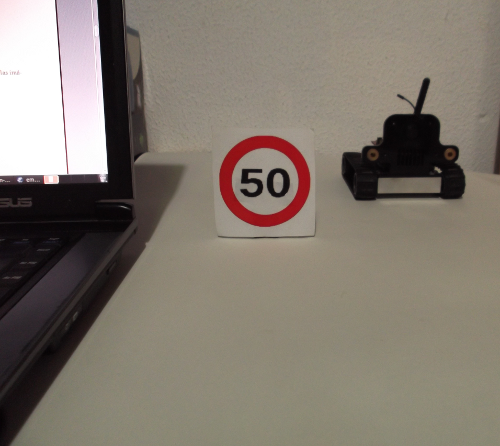
\includegraphics[scale=0.6]{im-entrada3.png}
  \end{center}
  \caption{Posible imagen de entrada al sistema.}
  \label{imagen-entrada-rp}
\end{figure}


\subsection{Extracción de características}
\label{sec:extraccion-caracteristicas}

Puesto que el fin es la detección de un objeto, la segmentación de la imagen es empleada para aislar en ella a todos los conjuntos de píxeles candidatos a ser el objeto a seguir o detectar. Como hemos visto en la imagen \ref{imagen-entrada-rp} las señales a detectar presentan colores llamativos, visualizándose en su contorno más externo los colores rojos y azules, siendo éstos los más representativos y predominantes. Por tanto resulta de especial utilidad la aplicación de una segmentación por color. Existen numerosos modelos de color utilizables para su realización como se ha descrito en la sección de \ref{def:modelos-color}.\\

Para la primera etapa del desarrollo del primer prototipo se ha empleado una técnica de segmentación por color siguiendo el modelo RGB. La finalidad de la segmentación es la de realizar una correcta selección de aquellos píxeles que según una determinada tonalidad resultan útiles para el posterior procesamiento e identificación de objetos. 

\subsubsection {Segmentación por color siguiendo el modelo RGB}
\label{sec:seg-color-rgb}

Dado que los colores predominantes de las señales a detectadas son los rojos y azules intensos se ha optado por la selección de ambas tonalidades, centrándonos, para este primer prototipo, en el color rojo exclusivamente.\\

Una vez decidido el color a identificar, resulta necesario conocer las tonalidades exactas y cómo ésta es representada por el ordenador. La solución fue crear una herramienta con la que al pinchar sobre una imagen, obtuviera de forma automática el color sobre el que se ha pulsado mostrando por pantalla el código del color en los tres canales: rojo, verde y azul. El programa se escribió en lenguaje C haciendo uso de la biblioteca OpenCV.\\

 En la figura \ref{fig:color-pixel} se puede observar el funcionamiento del programa mostrando el color sobre el que se ha hecho click, apreciándose como el último color seleccionado posee los valores 84, 70 y 202. Destacar que OpenCV invierte el orden de las componente empleando BGR en lugar de RGB. Es decir, azul, verde y rojo, presentando, por tanto, un valor numérico mayor en la tercera componente. Esto se debe a que el píxel pulsado en la imagen se corresponde con el contorno exterior de la señal de 50 km/h cuya tonalidad es roja y que predomina sobre las otras dos.\\

\begin{figure}[H]
  \begin{center}
    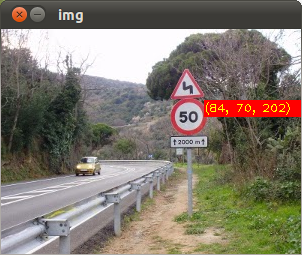
\includegraphics[scale=0.7]{color-pixel.png}
  \end{center}
  \caption{Programa elaborado para la obtención de los valores del píxel pulsado.}
  \label{fig:color-pixel}
\end{figure}

El código del programa elaborado se muestra a continuación:\\

\underline{Programa elaborado para la obtención del valor de un píxel en una imagen}\\
\begin{Verbatim}[commandchars=\\\{\}]
\PY{c+cp}{#}\PY{c+cp}{include "cv.h"}
\PY{c+cp}{#}\PY{c+cp}{include "highgui.h"}
\PY{c+cp}{#}\PY{c+cp}{include <stdio.h>}
\PY{c+cp}{#}\PY{c+cp}{include <stdlib.h>}

\PY{k+kt}{void} \PY{n+nf}{mouseHandler}\PY{p}{(}\PY{k+kt}{int} \PY{n}{event}\PY{p}{,} \PY{k+kt}{int} \PY{n}{x}\PY{p}{,} \PY{k+kt}{int} \PY{n}{y}\PY{p}{,} \PY{k+kt}{int} \PY{n}{flags}\PY{p}{,} \PY{k+kt}{void}\PY{o}{*} \PY{n}{param}\PY{p}{)}
\PY{p}{\PYZob{}}
    \PY{c+c1}{// Declaración de variables.}
    \PY{n}{IplImage}\PY{o}{*} \PY{n}{img0}\PY{p}{,} \PY{o}{*} \PY{n}{img1}\PY{p}{;}
    \PY{n}{CvFont}    \PY{n}{font}\PY{p}{;}
    \PY{n}{uchar}\PY{o}{*}    \PY{n}{ptr}\PY{p}{;}
    \PY{k+kt}{char}      \PY{n}{label}\PY{p}{[}\PY{l+m+mi}{20}\PY{p}{]}\PY{p}{;}

    \PY{n}{img0} \PY{o}{=} \PY{p}{(}\PY{n}{IplImage}\PY{o}{*}\PY{p}{)} \PY{n}{param}\PY{p}{;}
    \PY{n}{img1} \PY{o}{=} \PY{n}{cvCloneImage}\PY{p}{(}\PY{n}{img0}\PY{p}{)}\PY{p}{;}


    \PY{n}{cvInitFont}\PY{p}{(}\PY{o}{&}\PY{n}{font}\PY{p}{,} \PY{n}{CV\PYZus{}FONT\PYZus{}HERSHEY\PYZus{}PLAIN}\PY{p}{,} \PY{l+m+mf}{.8}\PY{p}{,} \PY{l+m+mf}{.8}\PY{p}{,} \PY{l+m+mi}{0}\PY{p}{,} \PY{l+m+mi}{1}\PY{p}{,} \PY{l+m+mi}{8}\PY{p}{)}\PY{p}{;}

    \PY{k}{if} \PY{p}{(}\PY{n}{event} \PY{o}{=}\PY{o}{=} \PY{n}{CV\PYZus{}EVENT\PYZus{}LBUTTONDOWN}\PY{p}{)}
    \PY{p}{\PYZob{}}
        \PY{c+c1}{// Se realiza la lectura del píxel pulsado.}
        \PY{n}{ptr} \PY{o}{=} \PY{n}{cvPtr2D}\PY{p}{(}\PY{n}{img1}\PY{p}{,} \PY{n}{y}\PY{p}{,} \PY{n}{x}\PY{p}{,} \PY{n+nb}{NULL}\PY{p}{)}\PY{p}{;}

        \PY{c+c1}{// Se muestra el valor RGB.}
        \PY{n}{sprintf}\PY{p}{(}\PY{n}{label}\PY{p}{,} \PY{l+s}{"}\PY{l+s}{(%d, %d, %d)}\PY{l+s}{"}\PY{p}{,} \PY{n}{ptr}\PY{p}{[}\PY{l+m+mi}{0}\PY{p}{]}\PY{p}{,} \PY{n}{ptr}\PY{p}{[}\PY{l+m+mi}{1}\PY{p}{]}\PY{p}{,} \PY{n}{ptr}\PY{p}{[}\PY{l+m+mi}{2}\PY{p}{]}\PY{p}{)}\PY{p}{;}
        
        \PY{c+c1}{// Se crea un rectángulo de color en la imagen...}
        \PY{n}{cvRectangle}\PY{p}{(} 
            \PY{n}{img1}\PY{p}{,}
            \PY{n}{cvPoint}\PY{p}{(}\PY{n}{x}\PY{p}{,} \PY{n}{y} \PY{o}{-} \PY{l+m+mi}{12}\PY{p}{)}\PY{p}{,}
            \PY{n}{cvPoint}\PY{p}{(}\PY{n}{x} \PY{o}{+} \PY{l+m+mi}{100}\PY{p}{,} \PY{n}{y} \PY{o}{+} \PY{l+m+mi}{4}\PY{p}{)}\PY{p}{,}
            \PY{n}{CV\PYZus{}RGB}\PY{p}{(}\PY{l+m+mi}{255}\PY{p}{,} \PY{l+m+mi}{0}\PY{p}{,} \PY{l+m+mi}{0}\PY{p}{)}\PY{p}{,}
            \PY{n}{CV\PYZus{}FILLED}\PY{p}{,}
            \PY{l+m+mi}{8}\PY{p}{,} \PY{l+m+mi}{0}
        \PY{p}{)}\PY{p}{;}
        \PY{c+c1}{// Y se dibuja los valores numéricos en su interior.}
        \PY{n}{cvPutText}\PY{p}{(}
            \PY{n}{img1}\PY{p}{,}
            \PY{n}{label}\PY{p}{,}
            \PY{n}{cvPoint}\PY{p}{(}\PY{n}{x}\PY{p}{,} \PY{n}{y}\PY{p}{)}\PY{p}{,}
            \PY{o}{&}\PY{n}{font}\PY{p}{,}
            \PY{n}{CV\PYZus{}RGB}\PY{p}{(}\PY{l+m+mi}{255}\PY{p}{,} \PY{l+m+mi}{255}\PY{p}{,} \PY{l+m+mi}{0}\PY{p}{)}
        \PY{p}{)}\PY{p}{;}

        \PY{c+c1}{// Finalmente se muestra la imagen.}
        \PY{n}{cvShowImage}\PY{p}{(}\PY{l+s}{"}\PY{l+s}{img}\PY{l+s}{"}\PY{p}{,} \PY{n}{img1}\PY{p}{)}\PY{p}{;}
    \PY{p}{\PYZcb{}}
\PY{p}{\PYZcb{}}


\PY{k+kt}{int} \PY{n}{main}\PY{p}{(}\PY{k+kt}{int} \PY{n}{argc}\PY{p}{,} \PY{k+kt}{char} \PY{o}{*}\PY{n}{argv}\PY{p}{[}\PY{p}{]}\PY{p}{)}\PY{p}{\PYZob{}}

    \PY{n}{IplImage}\PY{o}{*} \PY{n}{img}\PY{p}{,}\PY{o}{*}\PY{n}{hsv\PYZus{}image}\PY{p}{;}

    \PY{c+c1}{// Se comprueba que se ha introducido un argumento.}
    \PY{k}{if} \PY{p}{(}\PY{n}{argc} \PY{o}{!}\PY{o}{=} \PY{l+m+mi}{2}\PY{p}{)} \PY{p}{\PYZob{}}
        \PY{n}{printf}\PY{p}{(}\PY{l+s}{"}\PY{l+s}{Usage: %s <image>}\PY{l+s+se}{\PYZbs{}n}\PY{l+s}{"}\PY{p}{,} \PY{n}{argv}\PY{p}{[}\PY{l+m+mi}{0}\PY{p}{]}\PY{p}{)}\PY{p}{;}
        \PY{k}{return} \PY{l+m+mi}{1}\PY{p}{;}
    \PY{p}{\PYZcb{}}

    \PY{c+c1}{// Se realiza la carga de la imagen a partir de la ruta pasada }
    \PY{c+c1}{// como argumento de entrada.}
    \PY{n}{img} \PY{o}{=} \PY{n}{cvLoadImage}\PY{p}{(}\PY{n}{argv}\PY{p}{[}\PY{l+m+mi}{1}\PY{p}{]}\PY{p}{,} \PY{l+m+mi}{1}\PY{p}{)}\PY{p}{;}

    \PY{c+c1}{//Copia de la imagen de entrada en una nueva imagen.}
    \PY{n}{hsv\PYZus{}image} \PY{o}{=} \PY{n}{cvCloneImage}\PY{p}{(}\PY{n}{img}\PY{p}{)}\PY{p}{;} 
    
    \PY{c+c1}{//Transformacion a HSV}
    \PY{n}{cvCvtColor}\PY{p}{(}\PY{n}{img}\PY{p}{,} \PY{n}{hsv\PYZus{}image}\PY{p}{,} \PY{n}{CV\PYZus{}BGR2HSV}\PY{p}{)}\PY{p}{;}

    \PY{c+c1}{// Se crea una ventana con los eventos del ratón.}
    \PY{n}{cvNamedWindow}\PY{p}{(}\PY{l+s}{"}\PY{l+s}{img}\PY{l+s}{"}\PY{p}{,} \PY{l+m+mi}{1}\PY{p}{)}\PY{p}{;}
    \PY{n}{cvSetMouseCallback}\PY{p}{(}\PY{l+s}{"}\PY{l+s}{img}\PY{l+s}{"}\PY{p}{,} \PY{n}{mouseHandler}\PY{p}{,} \PY{p}{(}\PY{k+kt}{void}\PY{o}{*}\PY{p}{)}\PY{n}{hsv\PYZus{}image}\PY{p}{)}\PY{p}{;}

    \PY{n}{cvShowImage}\PY{p}{(}\PY{l+s}{"}\PY{l+s}{img}\PY{l+s}{"}\PY{p}{,} \PY{n}{hsv\PYZus{}image}\PY{p}{)}\PY{p}{;}
    \PY{n}{cvWaitKey}\PY{p}{(}\PY{l+m+mi}{0}\PY{p}{)}\PY{p}{;}

    \PY{c+c1}{// Eliminación de estructuras.}
    \PY{n}{cvDestroyAllWindows}\PY{p}{(}\PY{p}{)}\PY{p}{;}
    \PY{n}{cvReleaseImage}\PY{p}{(}\PY{o}{&}\PY{n}{img}\PY{p}{)}\PY{p}{;}
    \PY{n}{cvReleaseImage}\PY{p}{(}\PY{o}{&}\PY{n}{hsv\PYZus{}image}\PY{p}{)}\PY{p}{;}

    \PY{k}{return} \PY{l+m+mi}{0}\PY{p}{;}
\PY{p}{\PYZcb{}}
\end{Verbatim}


Una vez conocidos los umbrales sobre los que trabajar, siempre en torno a un pequeño margen, se procede a una criba de píxeles que entran dentro del citado rango.\\

El código mostrado a continuación recibe una imagen de entrada realizando su recorrido y activando en una nueva imagen binaria, originalmente inicializada a cero, con el valor 1 aquellos píxeles situados dentro del umbral de color indicado. El recorrido de la imagen se ha realizado utilizando la aritmética de punteros en lugar de las funciones consultoras propias de OpenCV con el fin de ganar en eficiencia.\\

\underline{Segmentación de una imagen siguiendo el modelo de color RGB}\\
\begin{Verbatim}[commandchars=\\\{\}]
\PY{n}{IplImage}\PY{o}{*} \PY{n}{segmentacion\PYZus{}RGB}\PY{p}{(}\PY{n}{IplImage}\PY{o}{*} \PY{n}{img}\PY{p}{)}\PY{p}{\PYZob{}}

  \PY{c+c1}{// Declaración de variables.}
  \PY{k+kt}{int} \PY{n}{altura}\PY{p}{,}\PY{n}{anchura}\PY{p}{,}\PY{n}{anchura\PYZus{}fila}\PY{p}{,}\PY{n}{canales}\PY{p}{;}
  \PY{n}{uchar} \PY{o}{*}\PY{n}{data}\PY{p}{;}
  \PY{k+kt}{int} \PY{n}{i}\PY{p}{,}\PY{n}{j}\PY{p}{;}
  
  \PY{c+c1}{// Recopilación de los datos de la imagen de entrada.}
  \PY{n}{altura} \PY{o}{=} \PY{n}{img}\PY{o}{-}\PY{o}{>}\PY{n}{height}\PY{p}{;}
  \PY{n}{anchura} \PY{o}{=} \PY{n}{img}\PY{o}{-}\PY{o}{>}\PY{n}{width}\PY{p}{;}
  \PY{n}{anchura\PYZus{}fila} \PY{o}{=} \PY{n}{img}\PY{o}{-}\PY{o}{>}\PY{n}{widthStep}\PY{p}{;}
  \PY{n}{canales} \PY{o}{=} \PY{n}{img}\PY{o}{-}\PY{o}{>}\PY{n}{nChannels}\PY{p}{;}
  \PY{n}{data} \PY{o}{=} \PY{p}{(}\PY{n}{uchar} \PY{o}{*}\PY{p}{)}\PY{n}{img}\PY{o}{-}\PY{o}{>}\PY{n}{imageData}\PY{p}{;}
     
  \PY{c+c1}{// Declaración e inicialización a cero de la imagen de salida.}
  \PY{n}{IplImage}\PY{o}{*} \PY{n}{img\PYZus{}selec\PYZus{}color}\PY{p}{;}  
  \PY{n}{img\PYZus{}selec\PYZus{}color} \PY{o}{=} \PY{n}{cvCreateImage}\PY{p}{(}\PY{n}{cvGetSize}\PY{p}{(}\PY{n}{img}\PY{p}{)}\PY{p}{,} \PY{n}{IPL\PYZus{}DEPTH\PYZus{}8U}\PY{p}{,}\PY{l+m+mi}{1}\PY{p}{)}\PY{p}{;}
  \PY{n}{cvZero}\PY{p}{(}\PY{n}{img\PYZus{}selec\PYZus{}color}\PY{p}{)}\PY{p}{;}

  \PY{c+c1}{// Recorrido de la imagen de entrada.}
  \PY{k}{for}\PY{p}{(}\PY{n}{i}\PY{o}{=}\PY{l+m+mi}{0}\PY{p}{;}\PY{n}{i}\PY{o}{<}\PY{n}{altura}\PY{p}{;}\PY{n}{i}\PY{o}{+}\PY{o}{+}\PY{p}{)}\PY{p}{\PYZob{}} 
    \PY{k}{for}\PY{p}{(}\PY{n}{j}\PY{o}{=}\PY{l+m+mi}{0}\PY{p}{;}\PY{n}{j}\PY{o}{<}\PY{n}{anchura}\PY{p}{;}\PY{n}{j}\PY{o}{+}\PY{o}{+}\PY{p}{)}\PY{p}{\PYZob{}}
      
      \PY{c+c1}{// Selección de tonalidades rojas.}
      \PY{k}{if} \PY{p}{(}\PY{p}{(}\PY{n}{data}\PY{p}{[}\PY{n}{i}\PY{o}{*}\PY{n}{anchura\PYZus{}fila}\PY{o}{+}\PY{n}{j}\PY{o}{*}\PY{n}{canales} \PY{o}{+} \PY{l+m+mi}{2}\PY{p}{]} \PY{o}{>} \PY{l+m+mi}{80}\PY{p}{)} \PY{o}{&}\PY{o}{&}
	  \PY{o}{!}\PY{p}{(}\PY{p}{(}\PY{n}{data}\PY{p}{[}\PY{n}{i}\PY{o}{*}\PY{n}{anchura\PYZus{}fila}\PY{o}{+}\PY{n}{j}\PY{o}{*}\PY{n}{canales} \PY{o}{+} \PY{l+m+mi}{0}\PY{p}{]} \PY{o}{>} 
            \PY{n}{data}\PY{p}{[}\PY{n}{i}\PY{o}{*}\PY{n}{anchura\PYZus{}fila}\PY{o}{+}\PY{n}{j}\PY{o}{*}\PY{n}{canales} \PY{o}{+} \PY{l+m+mi}{2}\PY{p}{]}\PY{o}{/}\PY{l+m+mi}{2}\PY{p}{)} \PY{o}{|}\PY{o}{|} 
	   \PY{p}{(}\PY{n}{data}\PY{p}{[}\PY{n}{i}\PY{o}{*}\PY{n}{anchura\PYZus{}fila}\PY{o}{+}\PY{n}{j}\PY{o}{*}\PY{n}{canales} \PY{o}{+} \PY{l+m+mi}{1}\PY{p}{]} \PY{o}{>} 
            \PY{n}{data}\PY{p}{[}\PY{n}{i}\PY{o}{*}\PY{n}{anchura\PYZus{}fila}\PY{o}{+}\PY{n}{j}\PY{o}{*}\PY{n}{canales} \PY{o}{+} \PY{l+m+mi}{2}\PY{p}{]}\PY{o}{/}\PY{l+m+mi}{2}\PY{p}{)}\PY{p}{)}\PY{p}{)} \PY{p}{\PYZob{}}
    
        \PY{c+c1}{//Activación de los píxeles que cumplen la condición de color fijada.}
	\PY{n}{img\PYZus{}selec\PYZus{}color}\PY{o}{-}\PY{o}{>}\PY{n}{imageData}\PY{p}{[} \PY{n}{img\PYZus{}selec\PYZus{}color}\PY{o}{-}\PY{o}{>}\PY{n}{widthStep} \PY{o}{*} \PY{n}{i} \PY{o}{+} \PY{n}{j} \PY{o}{*} \PY{l+m+mi}{1}\PY{p}{]}\PY{o}{=}\PY{l+m+mi}{1}\PY{p}{;}
      \PY{p}{\PYZcb{}}
    \PY{p}{\PYZcb{}}
  \PY{p}{\PYZcb{}}
  
  \PY{c+c1}{// Erosión para la eliminación de píxeles sueltos.}
  \PY{n}{cvErode}\PY{p}{(}\PY{n}{img\PYZus{}selec\PYZus{}color}\PY{p}{,} \PY{n}{img\PYZus{}selec\PYZus{}color}\PY{p}{,}\PY{n+nb}{NULL}\PY{p}{,}\PY{l+m+mi}{1}\PY{p}{)}\PY{p}{;}
  
  \PY{c+c1}{// Dilatación para expandir los objetos de la imagen.}
  \PY{n}{cvDilate}\PY{p}{(}\PY{n}{img\PYZus{}selec\PYZus{}color}\PY{p}{,}\PY{n}{img\PYZus{}selec\PYZus{}color}\PY{p}{,}\PY{n+nb}{NULL}\PY{p}{,}\PY{l+m+mi}{3}\PY{p}{)}\PY{p}{;}

  \PY{c+c1}{// Se devuelve la imagen resultante.	     }
  \PY{k}{return} \PY{n}{img\PYZus{}selec\PYZus{}color}\PY{p}{;}
\PY{p}{\PYZcb{}}
\end{Verbatim}


Una posible imagen de salida obtenida tras la aplicación del algoritmo de segmentación por color anterior se puede apreciar en la figura \ref{fig:ejemplo-selec-color} de a continuación:\\
 
\begin{figure}[H]
  \begin{center}
      \begin{tabular}{cc p{7cm}p{7cm}}
        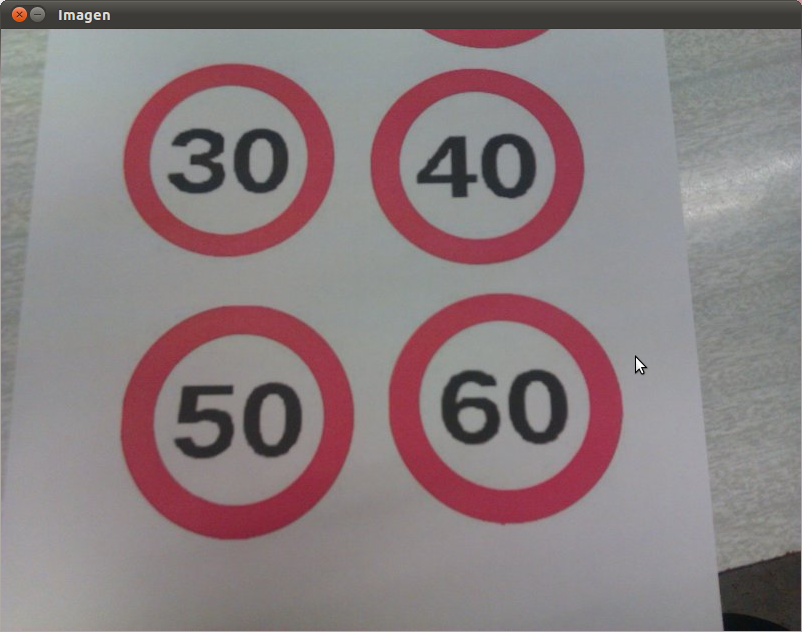
\includegraphics[width=7cm]{./imagenes/im-entrada.png} & 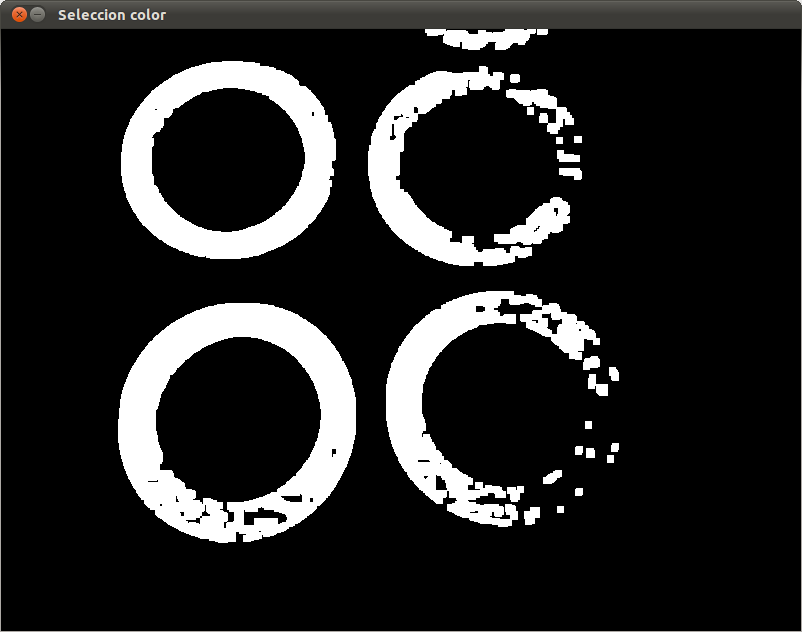
\includegraphics[width=7cm]{./imagenes/paso0.png}\\
        {Imagen de entrada (a).} & {Imagen resultante (b).}\\
      \end{tabular}
    \caption{Resultado de aplicar una selección por color sobre una imagen.}
    \label{fig:ejemplo-selec-color}
  \end{center}
\end{figure}

En la imagen \ref{fig:ejemplo-selec-color} de salida se puede apreciar un conjunto de objetos resultantes a los se les debe de aplicar algún mecanismo que permita trabajar con cada uno de los diferentes elementos por separado con la finalidad de poder clasificar cada uno de ellos de manera independiente.

\subsubsection {Extracción de objetos}
\label{sec:extraccion-objetos}

Una vez obtenida las agrupaciones de píxeles de tonalidad roja, figura \ref{fig:ejemplo-selec-color}, se procede a la identificación de cada una de esas agrupaciones por separado. Para ello utilizamos un método basado en la detección de contornos propio de OpenCV que está basado en el algoritmo de Canny. La aplicación de esta técnica nos permite averiguar los contornos de la imagen o, dicho de otro modo, los cambios bruscos de intensidades lumínicas.\\

Del paso anterior se obtiene una estructura tipo lista donde se encuentran almacenados todos los objetos detectados. El primer paso aplicado es descartar aquellos objetos cuyos valores de área son demasiado pequeños como para ser algunos de los elementos buscados, evitando así continuar con su análisis.\\

Los objetos restantes son, cada uno de ellos, encerrados dentro de una estructura rectangular de área mínima conociendo así su tamaño y coordenadas de localización.\\

Una vez conocidas las coordenadas que encierran al objeto, se establece una región de interés (ROI) en la imagen de entrada y en la obtenida tras la selección por color. Una región de interés es un área rectangular en una imagen, obteniendo el objeto segmentado para su posterior procesamiento. La figura \ref{fig:roi} muestra un claro ejemplo de una delimitación de una región de interés en una imagen.\\

\begin{figure}[H]
  \begin{center}
    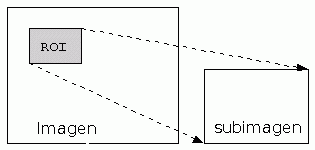
\includegraphics[scale=1]{roi.png}
  \end{center}
  \caption{Imagen con una región definida de interés.}
  \label{fig:roi}
\end{figure}

Cuando es asignada una región de interés en una imagen, todas las modificaciones realizadas sobre dicha imagen serán aplicadas sobre la zona seleccionada, una vez terminado el proceso de identificación del objeto encerrado en la región, ésta se libera y se procede a trabajar con una nueva región de interés en caso de existir más objetos candidatos a análisis en la imagen de entrada.\\

Una vez definidas las regiones de interés sobre ambas imágenes de la figura \ref{fig:ejemplo-selec-color}, se desea obtener la señal de forma independiente sin el fondo, para ello se emplea la técnica de copia usando una máscara, que no es más que copiar aquellos píxeles en una nueva imagen que se encuentren marcados en la imagen máscara. La imagen máscara es obtenida rellenando los huecos interiores de la imagen obtenida tras la aplicación de la selección por color. La figura \ref{fig:mascaras} muestra un ejemplo ilustrativo:\\

\begin{figure}[H]
  \begin{center}
      \begin{tabular}{ccc p{3cm}p{3cm}p{3cm}}
        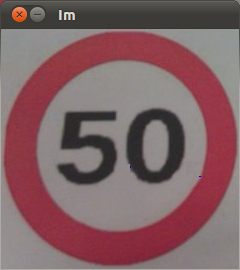
\includegraphics[width=3cm]{./imagenes/mascara/mascara1.png} &  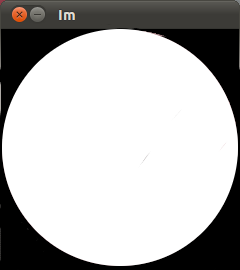
\includegraphics[width=3cm]{./imagenes/mascara/mascara2.png} & 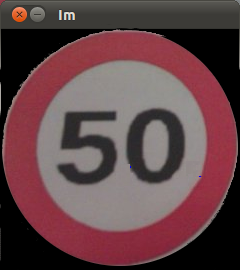
\includegraphics[width=3cm]{./imagenes/mascara/mascara3.png} \\
        {(\emph{a})} & {(\emph{b})} & {(\emph{c})} \\
      \end{tabular}
    \caption{Copia de una imagen mediante el uso de máscaras.}
    \label{fig:mascaras}
  \end{center}
\end{figure}

El código mostrado realiza las acciones de extracción de cada uno de los objetos por separado una vez aplicada la segmentación por color:\\

\underline{Código para la extracción de los objetos de una imagen}\\
\begin{Verbatim}[commandchars=\\\{\}]
\PY{c+c1}{// Segmentación por color}
\PY{n}{img\PYZus{}selec\PYZus{}color} \PY{o}{=} \PY{n}{segmentacion\PYZus{}RGB}\PY{p}{(}\PY{n}{img}\PY{p}{)}\PY{p}{;}

\PY{n}{dst} \PY{o}{=} \PY{n}{cvCreateImage}\PY{p}{(} \PY{n}{cvGetSize}\PY{p}{(}\PY{n}{img}\PY{p}{)}\PY{p}{,}\PY{n}{IPL\PYZus{}DEPTH\PYZus{}8U}\PY{p}{,} \PY{l+m+mi}{1} \PY{p}{)}\PY{p}{;}
\PY{n}{cvZero}\PY{p}{(}\PY{n}{dst}\PY{p}{)}\PY{p}{;}

\PY{c+c1}{// Búsqueda de contornos en la imagen obtenida tras la selección por color.}
\PY{n}{cvFindContours}\PY{p}{(}\PY{n}{img\PYZus{}selec\PYZus{}color}\PY{p}{,} \PY{n}{storage}\PY{p}{,} \PY{o}{&}\PY{n}{contour}\PY{p}{,} \PY{k}{sizeof}\PY{p}{(}\PY{n}{CvContour}\PY{p}{)}\PY{p}{,}
\PY{n}{CV\PYZus{}RETR\PYZus{}EXTERNAL}\PY{p}{,} \PY{n}{CV\PYZus{}CHAIN\PYZus{}APPROX\PYZus{}NONE}\PY{p}{)}\PY{p}{;}

\PY{n}{senial} \PY{o}{=} \PY{n}{cvCreateImage}\PY{p}{(}\PY{n}{cvGetSize}\PY{p}{(}\PY{n}{img}\PY{p}{)}\PY{p}{,} \PY{n}{IPL\PYZus{}DEPTH\PYZus{}8U}\PY{p}{,} \PY{l+m+mi}{3}\PY{p}{)}\PY{p}{;}
\PY{n}{cvZero}\PY{p}{(}\PY{n}{senial}\PY{p}{)}\PY{p}{;}     

\PY{c+c1}{// Para objeto encontrado:}
\PY{k}{for}\PY{p}{(}\PY{p}{;} \PY{n}{contour} \PY{o}{!}\PY{o}{=} \PY{l+m+mi}{0}\PY{p}{;} \PY{n}{contour} \PY{o}{=} \PY{n}{contour}\PY{o}{-}\PY{o}{>}\PY{n}{h\PYZus{}next} \PY{p}{)}\PY{p}{\PYZob{}}
  
  \PY{c+c1}{// Se calcula su área.}
  \PY{n}{area}\PY{o}{=}\PY{n}{fabs}\PY{p}{(}\PY{n}{cvContourArea}\PY{p}{(}\PY{n}{contour}\PY{p}{,}\PY{n}{CV\PYZus{}WHOLE\PYZus{}SEQ}\PY{p}{)}\PY{p}{)}\PY{p}{;}
  
  \PY{c+c1}{// Si el área supera un determinado valor de área. }
  \PY{k}{if}\PY{p}{(}\PY{n}{area}\PY{o}{>}\PY{o}{=}\PY{l+m+mi}{300}\PY{p}{)}\PY{p}{\PYZob{}}
    
    \PY{c+c1}{// Se dibuja el objeto en una imagen.}
    \PY{n}{cvDrawContours}\PY{p}{(}\PY{n}{dst}\PY{p}{,} \PY{n}{contour}\PY{p}{,} \PY{n}{cvScalar}\PY{p}{(}\PY{l+m+mi}{1}\PY{p}{)}\PY{p}{,}\PY{n}{cvScalar}\PY{p}{(}\PY{l+m+mi}{1}\PY{p}{)}\PY{p}{,} \PY{o}{-}\PY{l+m+mi}{1}\PY{p}{,} \PY{n}{CV\PYZus{}FILLED}\PY{p}{,} \PY{l+m+mi}{8}\PY{p}{)}\PY{p}{;}
    
    \PY{c+c1}{// Se calcula el área mínima que encierra al objeto.}
    \PY{n}{rect} \PY{o}{=} \PY{n}{cvBoundingRect}\PY{p}{(}\PY{n}{contour}\PY{p}{,}\PY{l+m+mi}{0}\PY{p}{)}\PY{p}{;} 
    
    \PY{c+c1}{// Selección de las regiones de interés.}
    \PY{n}{cvSetImageROI}\PY{p}{(}\PY{n}{dst}\PY{p}{,}\PY{n}{rect}\PY{p}{)}\PY{p}{;}
    \PY{n}{cvSetImageROI}\PY{p}{(}\PY{n}{senial}\PY{p}{,}\PY{n}{rect}\PY{p}{)}\PY{p}{;}
    \PY{n}{cvSetImageROI}\PY{p}{(}\PY{n}{img}\PY{p}{,}\PY{n}{rect}\PY{p}{)}\PY{p}{;}
    
    \PY{c+c1}{// Se realiza la copia mediante la}
    \PY{c+c1}{// utilización de máscaras para eliminar el fondo del objeto.}
    \PY{n}{cvCopy}\PY{p}{(}\PY{n}{img}\PY{p}{,}\PY{n}{senial}\PY{p}{,}\PY{n}{dst}\PY{p}{)}\PY{p}{;}

    \PY{c+c1}{// Se eliminan las regiones de interés establecidas previamente.}
    \PY{n}{cvResetImageROI}\PY{p}{(}\PY{n}{dst}\PY{p}{)}\PY{p}{;}
    \PY{n}{cvResetImageROI}\PY{p}{(}\PY{n}{img}\PY{p}{)}\PY{p}{;}
    
    \PY{c+c1}{// Se redimensiona la imagen.}
    \PY{n}{identificar} \PY{o}{=} \PY{n}{cvCreateImage}\PY{p}{(} \PY{n}{cvSize}\PY{p}{(}\PY{l+m+mi}{100}\PY{p}{,}\PY{l+m+mi}{100}\PY{p}{)}\PY{p}{,}\PY{n}{IPL\PYZus{}DEPTH\PYZus{}8U}\PY{p}{,}\PY{l+m+mi}{3}\PY{p}{)}\PY{p}{;}
    \PY{n}{cvResize}\PY{p}{(}\PY{n}{senial}\PY{p}{,}\PY{n}{identificar}\PY{p}{,}\PY{n}{CV\PYZus{}INTER\PYZus{}LINEAR}\PY{p}{)}\PY{p}{;}
    
    \PY{c+c1}{// Y ya disponemos la imagen con el elemento a identificar.   }
    \PY{n}{cvShowImage}\PY{p}{(} \PY{l+s}{"}\PY{l+s}{Elemento}\PY{l+s}{"}\PY{p}{,}\PY{n}{identificar}\PY{p}{)}\PY{p}{;}

    \PY{c+c1}{// ALGORITMO IDENTIFICADOR}

  \PY{p}{\PYZcb{}} \PY{c+c1}{// Fin if.}
 \PY{p}{\PYZcb{}} \PY{c+c1}{// Fin for.}
\end{Verbatim}


Una vez obtenida una imagen independiente con el objeto a identificar en color, imagen \emph{c} de la figura \ref{fig:mascaras} o la variable identificar del código anterior, debe ser redimensionada para que todos los objetos a análisis sean de igual tamaño para proceder a la aplicación de la técnica de clasificación denominada ``Template matching'' o comparación de plantillas.

\subsection {Template matching}

Para la identificación de los objetos en el primer prototipo se ha utilizado una técnica denominada Template Matching o comparación de plantillas.\\

Esta técnica consiste en la búsqueda de la región de una imagen que mayor semejanza guarda con la imagen dada como plantilla.\\

En la comparación de plantillas, todas las posibles localizaciones que pueden ser comparadas con la plantilla son almacenadas en una matriz \emph{R}, en la cual se almacenan los coeficientes resultantes de las comparaciones. El tamaño de la imagen de entrada es de \emph{W} x \emph{H} donde \emph{W} y \emph{H} representan el ancho y el alto de la imagen respectivamente y \emph{w} x \emph{h} se corresponde con el producto del ancho por el alto de la imagen plantilla. El tamaño de la matriz viene dado por $(W - w + 1) x (H - h + 1)$. \\

\begin{figure}[H]
  \begin{center}
    \begin{tabular}{cc p{6.6cm}p{8cm}}
      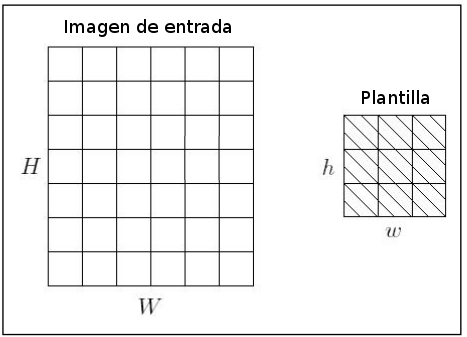
\includegraphics[width=6.6cm]{./imagenes/plantillas.png} &  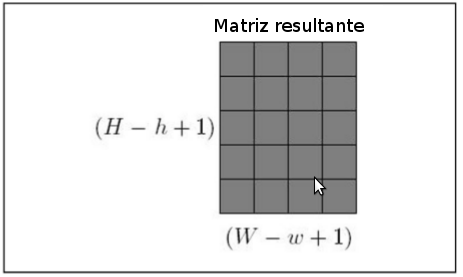
\includegraphics[width=8cm]{./imagenes/template-resultante.png} \\
                      {Matrices de origen (\emph{a}).} & {Matriz resultado (\emph{b}).} \\
    \end{tabular}
  \end{center}
  \caption{Matrices de entrada y de salida para la técnica de comparación de plantillas.}
\end{figure}
  \label{fig:template-in-out}

\begin{figure}[H]
  \begin{center}
    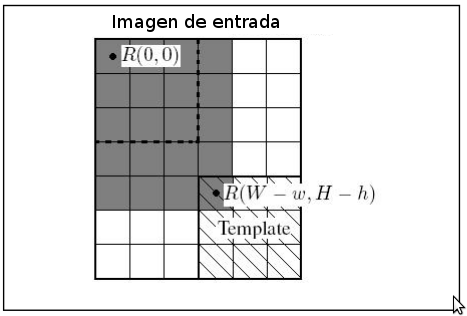
\includegraphics[scale=0.6]{ejemplo-template.png}
  \end{center}
  \caption{El valor de cada píxel de la posición $(x,y)$ es procesado para obtener su característica de similitud entre la plantilla y el rectángulo resultante de tomar $(x,y)$ como píxel situado en la esquina superior izquierda.}
  \label{fig:template}
\end{figure}

Las referencias del tamaño y la representación del proceso de comparación de plantillas se muestra en las figuras \ref{fig:template-in-out} (a) y \ref{fig:template}, respectivamente.\\

La figura \ref{fig:template-in-out} (b), muestra la matriz final obtenida tras el proceso de búsqueda de una plantilla en una imagen.\\

Existen varios métodos para la comparación de plantillas, algunos de los más conocidos son la suma de las diferencias al cuadrado, correlación cruzada y el método del Coeficiente de Correlación. Dependiendo del algoritmo, el resultado correspondiente puede ser ligeramente diferente. Se considera \emph{T} como la imagen de la plantilla e \emph{I} como la imagen de entrada. En el presente prototipo el método de las diferencias al cuadrado es el que ha resultado más eficaz. A continuación se muestra su fundamento matemático:\\

\begin{equation}
  R(x,y) = \frac{\sum_{x',y'} (T(x',y') - I(x+x',y+y'))^2} {\sqrt{\sum_{x',y'}T(x',y')^2 \cdot \sum_{x',y'}I(x+x',y+y')}} 
\label{eq:template-def}
\end{equation}

Los valores obtenidos tras aplicar \ref{eq:template-def} en cada píxel de la imagen de entrada son almacenados en una matriz de salida \emph{R} anteriormente descrita. Dicha matriz finalmente se recorre localizando aquellos valores que superen un umbral fijado con el fin de dar por localizado el objeto que se encontraba en la imagen que ha sido empleada como plantilla.\\
  
A continuación se muestra el código realizado en OpenCV para la comparación de plantillas:\\

\underline{Código para la detección de un objeto}\\
\begin{Verbatim}[commandchars=\\\{\}]
\PY{c+c1}{// ALGORITMO DE IDENTIFICACIÓN}

\PY{c+c1}{// Carga de imagen referencia o plantilla.}
\PY{n}{tpl} \PY{o}{=} \PY{n}{cvLoadImage}\PY{p}{(} \PY{n}{directorio}\PY{p}{,} \PY{n}{CV\PYZus{}LOAD\PYZus{}IMAGE\PYZus{}COLOR} \PY{p}{)}\PY{p}{;}

\PY{c+c1}{// Cáculo de ancho y alto de la imagen resultado.}
\PY{n}{width}  \PY{o}{=} \PY{n}{identificar}\PY{o}{-}\PY{o}{>}\PY{n}{width}  \PY{o}{-} \PY{n}{tpl}\PY{o}{-}\PY{o}{>}\PY{n}{width} \PY{o}{+} \PY{l+m+mi}{1}\PY{p}{;}
\PY{n}{height} \PY{o}{=} \PY{n}{identificar}\PY{o}{-}\PY{o}{>}\PY{n}{height} \PY{o}{-} \PY{n}{tpl}\PY{o}{-}\PY{o}{>}\PY{n}{height} \PY{o}{+} \PY{l+m+mi}{1}\PY{p}{;}

\PY{c+c1}{// Se crea la imagen donde se almacenará el resultado de la comparación.}
\PY{n}{res} \PY{o}{=} \PY{n}{cvCreateImage}\PY{p}{(} \PY{n}{cvSize}\PY{p}{(} \PY{n}{width}\PY{p}{,} \PY{n}{height} \PY{p}{)}\PY{p}{,} \PY{n}{IPL\PYZus{}DEPTH\PYZus{}32F}\PY{p}{,} \PY{l+m+mi}{1} \PY{p}{)}\PY{p}{;}

\PY{c+c1}{// Se realiza la comparación:}
\PY{n}{cvMatchTemplate}\PY{p}{(}\PY{n}{identificar}\PY{p}{,} \PY{n}{tpl}\PY{p}{,} \PY{n}{res}\PY{p}{,} \PY{n}{CV\PYZus{}TM\PYZus{}SQDIFF\PYZus{}NORMED}\PY{p}{)}\PY{p}{;}

\PY{k}{for}\PY{p}{(} \PY{n}{i} \PY{o}{=} \PY{l+m+mi}{0} \PY{p}{;} \PY{n}{i} \PY{o}{<} \PY{n}{height} \PY{p}{;} \PY{n}{i}\PY{o}{+}\PY{o}{+}\PY{p}{)} \PY{p}{\PYZob{}}
  \PY{k}{for}\PY{p}{(} \PY{n}{j} \PY{o}{=} \PY{l+m+mi}{0} \PY{p}{;} \PY{n}{j} \PY{o}{<} \PY{n}{width} \PY{p}{;} \PY{n}{j}\PY{o}{+}\PY{o}{+}\PY{p}{)} \PY{p}{\PYZob{}}

    \PY{c+c1}{// sacamos el elemento:}
    \PY{n}{s} \PY{o}{=} \PY{n}{cvGet2D}\PY{p}{(} \PY{n}{res}\PY{p}{,} \PY{n}{i}\PY{p}{,} \PY{n}{j} \PY{p}{)}\PY{p}{;}
    
    \PY{c+c1}{// Si el valor se localiza entre el rango establecido...}
    \PY{k}{if}\PY{p}{(} \PY{n}{s}\PY{p}{.}\PY{n}{val}\PY{p}{[}\PY{l+m+mi}{0}\PY{p}{]} \PY{o}{<}\PY{o}{=} \PY{n}{umbral} \PY{p}{)} \PY{p}{\PYZob{}}
      \PY{c+c1}{// Dibujamos el contorno al objeto identificado ENCONTRADO!}
      \PY{n}{fprintf}\PY{p}{(} \PY{n}{stderr}\PY{p}{,} \PY{l+s}{"}\PY{l+s}{¡50 m/h!}\PY{l+s}{"}\PY{p}{)}\PY{p}{;}
      
      \PY{n}{pt1}\PY{p}{.}\PY{n}{x} \PY{o}{=} \PY{n}{rect}\PY{p}{.}\PY{n}{x}\PY{p}{;}
      \PY{n}{pt1}\PY{p}{.}\PY{n}{y} \PY{o}{=} \PY{n}{rect}\PY{p}{.}\PY{n}{y}\PY{p}{;}
      \PY{n}{pt2}\PY{p}{.}\PY{n}{x} \PY{o}{=} \PY{n}{rect}\PY{p}{.}\PY{n}{x} \PY{o}{+} \PY{n}{rect}\PY{p}{.}\PY{n}{width}\PY{p}{;}
      \PY{n}{pt2}\PY{p}{.}\PY{n}{y} \PY{o}{=} \PY{n}{rect}\PY{p}{.}\PY{n}{y} \PY{o}{+} \PY{n}{rect}\PY{p}{.}\PY{n}{height}\PY{p}{;}
      
      \PY{c+c1}{// Se dibuja el rectángulo que encierra al objeto.}
      \PY{n}{cvRectangle}\PY{p}{(}\PY{n}{img}\PY{p}{,}\PY{n}{pt1}\PY{p}{,}\PY{n}{pt2}\PY{p}{,}\PY{n}{CV\PYZus{}RGB}\PY{p}{(}\PY{l+m+mi}{0}\PY{p}{,}\PY{l+m+mi}{255}\PY{p}{,}\PY{l+m+mi}{0}\PY{p}{)}\PY{p}{,}\PY{l+m+mi}{3}\PY{p}{,}\PY{l+m+mi}{8}\PY{p}{,}\PY{l+m+mi}{0}\PY{p}{)}\PY{p}{;}
    \PY{p}{\PYZcb{}}
  \PY{p}{\PYZcb{}}
 \PY{p}{\PYZcb{}}
\end{Verbatim}


La figura \ref{fig:detectado} muestra una imagen donde se aprecia cómo el objeto utilizado como plantilla ha sido detectado:\\

\begin{figure}[H]
  \begin{center}
    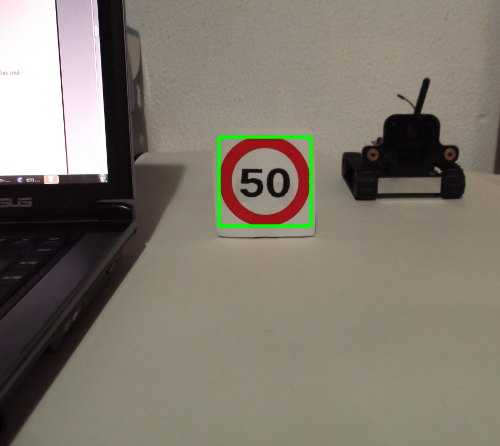
\includegraphics[scale=0.5]{detectado2.png}
  \end{center}
  \caption{Vista de la señal detectada en la imagen.}
  \label{fig:detectado}
\end{figure}

La técnica de comparación de plantillas, como se ha descrito, presenta la particularidad de encontrar un determinado objeto dentro de una imagen, por tanto, a priori el preprocesado previo realizado para aplicar una segmentación por color y extracción de los objetos por separado antes de emplear este algoritmo de clasificación no resulta necesario para su funcionamiento. El preprocesado previo se ha realizado para evitar las innecesarias comparaciones en zonas de la imagen donde sabemos que el objeto buscado no se va a encontrar, ganando por tanto en eficiencia.

\subsection{Problemas detectados}

Los problemas que han llevado a cabo el rechazo de este primer prototipo han sido los siguientes:

\begin{itemize}

\item El problema de la utilización de una segmentación por color siguiendo el modelo RGB es que sufre una extrema sensibilidad de variación de los valores de un determinado color a las condiciones lumínicas del entorno. Esto ocasiona que el prototipo desarrollado solo sea funcional en un único entorno, por ejemplo, la sala donde se ha desarrollado y probado, dejando de ser funcional en otras situaciones y lugares siendo necesario idear una nueva metodología de segmentación para el siguiente prototipo.

\item El problema del Template Matching es que ha de comparar muchas características (para él, un píxel es una característica), y si tenemos en cuenta que en la base de datos encontramos N señales, observamos que este método el resultado no ofrece garantías de funcionamiento en tiempo real, condición indispensable del proyecto.

\end{itemize}

\section{Segundo prototipo}

Este segundo prototipo difiere del anterior por la utilización para la segmentación por color del modelo de color HSV. Este modelo de color es mucho menos sensible a las condiciones lumínicas del entorno, permitiendo la detección de las tonalidades deseadas en situaciones donde el primer prototipo presentaba problemas.\\

Por otro lado, para la clasificación se ha optado por la utilización del algoritmo de los K-vecinos en lugar de la comparación de plantillas o Template Matching.\\

Destacar que para la función del algoritmo de los k-vecinos resulta necesaria una recolección previa de los datos de los elementos a detectar, los denominados clases, con el fin de realizar una serie de comparaciones entre el objeto desconocido y los datos previamente extraídos con la finalidad de determinar a que clase corresponde. Por tanto se describirá el algoritmo de entrenamiento (extracción de datos) y el algoritmo de detección (clasificación) utilizados.

\subsection{Extracción de características}

Para poder clasificar satisfactoriamente los elementos, es necesario un proceso de aprendizaje previo en el cual el sistema crea un modelo de cada una de las clases a partir de una secuencia de entrenamiento o conjunto de vectores de características de cada una de las clases.\\

Debido a esta razón, debemos previamente, antes de realizar cualquier tarea de clasificación, elaborar un conjunto de vectores de características o también denominado matriz de modelos con el fin de cotejar las características del elemento a identificar con los datos de la matriz modelos. A la fase de obtención de la matriz de modelos se le denomina etapa de entrenamiento en un sistema de reconocimiento de patrones. Dicha matriz ha sido obtenida en una serie de etapas que se describen en los sucesivos puntos de esta sección. 

\subsubsection {Segmentación por color siguiendo el modelo HSV}
\label{sec:color-HSV}

En la primera etapa del entrenamiento se ha optado por continuar con una técnica de segmentación por color, pero en esta ocasión siguiendo el modelo HSV. Cabe recordar que la finalidad de la segmentación es la de realizar una correcta selección de aquellos píxeles que según una determinada tonalidad resultan útiles para el posterior procesamiento e identificación de objetos.\\

En esta ocasión se presenta el mismo problema que con el primer prototipo, se desconocen los valores correspondiente al color a identificar, siendo, de igual modo, necesario conocer las tonalidades exactas y cómo la susodicha tonalidad es representada por el ordenador. La solución en este caso fue adaptar la herramienta empleada en el primer prototipo. Dicha herramienta mostraba el valor de un determinado píxel al pulsar sobre el mismo, solo que en esta ocasión en formato HSV.  El código del programa es idéntico al mostrado en el primer prototipo pero realizando previamente una transformación de la imagen del formato RGB al formato HSV.\\

 En la figura \ref{fig:color-pixel2} se puede observar el funcionamiento del programa mostrando el color sobre el que se ha hecho click, apreciándose como el último color seleccionado posee los valores en sus tres canales: Hue, Saturation, Value, en castellano, tono, saturación y valor. Los valores obtenidos son (175,52,220) fijándonos en los valores correspondientes al tono y la saturación. El programa se escribió en lenguaje C haciendo uso de la biblioteca OpenCV.\\

\begin{figure}[H]
  \begin{center}
    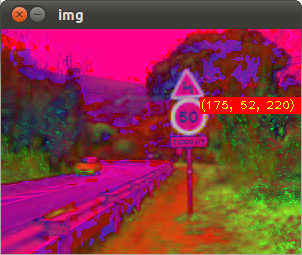
\includegraphics[scale=0.7]{color-pixel2.png}
  \end{center}
  \caption{Programa elaborado para la obtención de los valores del píxel pulsado.}
  \label{fig:color-pixel2}
\end{figure}

La aplicación de este modelo resulta mucho más ventajosa con respecto al modelo RGB debido a que HSV sólo precisa de un solo valor numérico para detectar el color, desde tonos relativamente ligeros hasta los tonos más oscuros. La cantidad de color y el brillo del color son manejados por la \emph{saturación} y los parámetros \emph{valor}, respectivamente.\\

A continuación se muestra el código realizado para realizar la segmentación por color de una imagen de entrada, en la cual, al igual que la función desarrollada para la segmentación siguiendo el modelo RGB, se han fijado unos umbrales y se ha recorrido la imagen identificando aquellos píxeles que cumplen las condiciones dejando el píxel activado en una imagen de salida.\\

\underline{Segmentación de una imagen siguiendo el modelo de color HSV}\\
\begin{Verbatim}[commandchars=\\\{\}]
\PY{n}{IplImage}\PY{o}{*} \PY{n}{seleccion\PYZus{}colorHSV}\PY{p}{(}\PY{n}{IplImage}\PY{o}{*} \PY{n}{img} \PY{p}{)}\PY{p}{\PYZob{}}

  \PY{c+c1}{// Declaración de variables}
  \PY{n}{IplImage} \PY{o}{*}\PY{n}{hsv\PYZus{}Image}\PY{p}{,} \PY{o}{*}\PY{n}{mono\PYZus{}Image}\PY{p}{;}
  \PY{k+kt}{int} \PY{n}{height} \PY{p}{,} \PY{n}{width} \PY{p}{,} \PY{n}{step} \PY{p}{,} \PY{n}{channels}\PY{p}{;}
  \PY{k+kt}{int} \PY{n}{step\PYZus{}mono} \PY{p}{,} \PY{n}{channels\PYZus{}mono}\PY{p}{;}  
  \PY{n}{uchar} \PY{o}{*}\PY{n}{data\PYZus{}hsv} \PY{p}{,} \PY{o}{*}\PY{n}{data\PYZus{}mono}\PY{p}{;}


  \PY{c+c1}{// Declaración de los valores umbral.}
  \PY{k+kt}{int} \PY{n}{hupper}\PY{o}{=}\PY{l+m+mi}{175}\PY{p}{,}\PY{n}{hlower}\PY{o}{=}\PY{l+m+mi}{110}\PY{p}{,}\PY{n}{Saturation}\PY{o}{=}\PY{l+m+mi}{60}\PY{p}{,}\PY{n}{Brightness}\PY{o}{=}\PY{l+m+mi}{90}\PY{p}{,}\PY{n}{Erode}\PY{o}{=}\PY{l+m+mi}{1}\PY{p}{,}\PY{n}{Dilate}\PY{o}{=}\PY{l+m+mi}{1}\PY{p}{;}

  \PY{k+kt}{int} \PY{n}{hupper2}\PY{o}{=}\PY{l+m+mi}{35}\PY{p}{,}\PY{n}{hlower2}\PY{o}{=}\PY{l+m+mi}{0}\PY{p}{,}\PY{n}{Saturation2}\PY{o}{=}\PY{l+m+mi}{60}\PY{p}{,}\PY{n}{Brightness2}\PY{o}{=}\PY{l+m+mi}{60}\PY{p}{,}\PY{n}{Erode2}\PY{o}{=}\PY{l+m+mi}{0}\PY{p}{,}\PY{n}{Dilate2}\PY{o}{=}\PY{l+m+mi}{3}\PY{p}{;}   
  \PY{c+c1}{//}

  \PY{c+c1}{// Se crean dos imágenes del tamaño de la imagen fuente.}
  \PY{n}{hsv\PYZus{}Image} \PY{o}{=} \PY{n}{cvCreateImage}\PY{p}{(} \PY{n}{cvGetSize}\PY{p}{(}\PY{n}{img}\PY{p}{)}\PY{p}{,} \PY{l+m+mi}{8}\PY{p}{,} \PY{l+m+mi}{3} \PY{p}{)}\PY{p}{;}
  \PY{n}{mono\PYZus{}Image} \PY{o}{=} \PY{n}{cvCreateImage}\PY{p}{(} \PY{n}{cvGetSize}\PY{p}{(}\PY{n}{img}\PY{p}{)}\PY{p}{,} \PY{l+m+mi}{8}\PY{p}{,} \PY{l+m+mi}{1} \PY{p}{)}\PY{p}{;}
  \PY{c+c1}{// Se inicializan a cero.}
  \PY{n}{cvZero}\PY{p}{(}\PY{n}{hsv\PYZus{}Image}\PY{p}{)}\PY{p}{;}
  \PY{n}{cvZero}\PY{p}{(}\PY{n}{mono\PYZus{}Image}\PY{p}{)}\PY{p}{;}

  \PY{c+c1}{// Obtenemos atributos de la imagen HSV.}
  \PY{n}{height}     \PY{o}{=} \PY{n}{hsv\PYZus{}Image}\PY{o}{-}\PY{o}{>}\PY{n}{height}\PY{p}{;}
  \PY{n}{width}      \PY{o}{=} \PY{n}{hsv\PYZus{}Image}\PY{o}{-}\PY{o}{>}\PY{n}{width}\PY{p}{;}
  \PY{n}{step}       \PY{o}{=} \PY{n}{hsv\PYZus{}Image}\PY{o}{-}\PY{o}{>}\PY{n}{widthStep}\PY{o}{/}\PY{k}{sizeof}\PY{p}{(}\PY{n}{uchar}\PY{p}{)}\PY{p}{;}
  \PY{n}{channels}   \PY{o}{=} \PY{n}{hsv\PYZus{}Image}\PY{o}{-}\PY{o}{>}\PY{n}{nChannels}\PY{p}{;}
  \PY{n}{step\PYZus{}mono}   \PY{o}{=} \PY{n}{mono\PYZus{}Image}\PY{o}{-}\PY{o}{>}\PY{n}{widthStep}\PY{o}{/}\PY{k}{sizeof}\PY{p}{(}\PY{n}{uchar}\PY{p}{)}\PY{p}{;}
  \PY{n}{channels\PYZus{}mono} \PY{o}{=} \PY{n}{mono\PYZus{}Image}\PY{o}{-}\PY{o}{>}\PY{n}{nChannels}\PY{p}{;}

  \PY{c+c1}{// Convertimos imagen de entrada de RGB a HSV.}
  \PY{n}{cvCvtColor}\PY{p}{(}\PY{n}{img}\PY{p}{,}\PY{n}{hsv\PYZus{}Image}\PY{p}{,}\PY{n}{CV\PYZus{}RGB2HSV}\PY{p}{)}\PY{p}{;}

  \PY{c+c1}{// Obtenemos los valores RGB de la Imagen.}
  \PY{n}{data\PYZus{}hsv} \PY{o}{=} \PY{p}{(}\PY{n}{uchar} \PY{o}{*}\PY{p}{)}\PY{n}{hsv\PYZus{}Image}\PY{o}{-}\PY{o}{>}\PY{n}{imageData}\PY{p}{;}
  \PY{n}{data\PYZus{}mono} \PY{o}{=} \PY{p}{(}\PY{n}{uchar} \PY{o}{*}\PY{p}{)}\PY{n}{mono\PYZus{}Image}\PY{o}{-}\PY{o}{>}\PY{n}{imageData}\PY{p}{;}

  \PY{c+c1}{//Recorremos la imagen.}
  \PY{k}{for}\PY{p}{(}\PY{k+kt}{int} \PY{n}{i} \PY{o}{=} \PY{l+m+mi}{0}\PY{p}{;} \PY{n}{i} \PY{o}{<}\PY{n}{height}\PY{p}{;} \PY{n}{i}\PY{o}{+}\PY{o}{+} \PY{p}{)} \PY{p}{\PYZob{}}
    \PY{k}{for}\PY{p}{(}\PY{k+kt}{int} \PY{n}{j} \PY{o}{=} \PY{l+m+mi}{0}\PY{p}{;} \PY{n}{j} \PY{o}{<}\PY{n}{width}\PY{p}{;} \PY{n}{j}\PY{o}{+}\PY{o}{+} \PY{p}{)} \PY{p}{\PYZob{}}

        \PY{c+c1}{// Segmentamos la imagen mediante los valores umbrales }
        \PY{c+c1}{// correspondientes al color rojo y azul.}
        \PY{k}{if} \PY{p}{(}\PY{p}{(}\PY{p}{(}\PY{n}{data\PYZus{}hsv}\PY{p}{[}\PY{n}{i}\PY{o}{*}\PY{n}{step}\PY{o}{+}\PY{n}{j}\PY{o}{*}\PY{n}{channels}\PY{p}{]}\PY{p}{)}\PY{o}{>}\PY{o}{=} \PY{n}{hlower}\PY{p}{)} \PY{o}{&}\PY{o}{&}
            \PY{p}{(}\PY{p}{(}\PY{n}{data\PYZus{}hsv}\PY{p}{[}\PY{n}{i}\PY{o}{*}\PY{n}{step}\PY{o}{+}\PY{n}{j}\PY{o}{*}\PY{n}{channels}\PY{p}{]}\PY{p}{)} \PY{o}{<}\PY{o}{=} \PY{n}{hupper}\PY{p}{)} \PY{o}{&}\PY{o}{&} 
            \PY{p}{(}\PY{n}{data\PYZus{}hsv}\PY{p}{[}\PY{n}{i}\PY{o}{*}\PY{n}{step}\PY{o}{+}\PY{n}{j}\PY{o}{*}\PY{n}{channels}\PY{o}{+}\PY{l+m+mi}{1}\PY{p}{]}\PY{o}{>}\PY{o}{=} \PY{n}{Saturation} \PY{p}{)} \PY{o}{&}\PY{o}{&} 
            \PY{p}{(}\PY{n}{data\PYZus{}hsv}\PY{p}{[}\PY{n}{i}\PY{o}{*}\PY{n}{step}\PY{o}{+}\PY{n}{j}\PY{o}{*}\PY{n}{channels}\PY{o}{+}\PY{l+m+mi}{2}\PY{p}{]}\PY{o}{>}\PY{o}{=} \PY{n}{Brightness}\PY{p}{)} \PY{o}{|}\PY{o}{|} 
            \PY{p}{(}\PY{p}{(}\PY{n}{data\PYZus{}hsv}\PY{p}{[}\PY{n}{i}\PY{o}{*}\PY{n}{step}\PY{o}{+}\PY{n}{j}\PY{o}{*}\PY{n}{channels}\PY{p}{]}\PY{p}{)}\PY{o}{>}\PY{o}{=} \PY{n}{hlower2}\PY{p}{)} \PY{o}{&}\PY{o}{&}
            \PY{p}{(}\PY{p}{(}\PY{n}{data\PYZus{}hsv}\PY{p}{[}\PY{n}{i}\PY{o}{*}\PY{n}{step}\PY{o}{+}\PY{n}{j}\PY{o}{*}\PY{n}{channels}\PY{p}{]}\PY{p}{)} \PY{o}{<}\PY{o}{=} \PY{n}{hupper2}\PY{p}{)} \PY{o}{&}\PY{o}{&} 
            \PY{p}{(}\PY{n}{data\PYZus{}hsv}\PY{p}{[}\PY{n}{i}\PY{o}{*}\PY{n}{step}\PY{o}{+}\PY{n}{j}\PY{o}{*}\PY{n}{channels}\PY{o}{+}\PY{l+m+mi}{1}\PY{p}{]}\PY{o}{>}\PY{o}{=} \PY{n}{Saturation2} \PY{p}{)} \PY{o}{&}\PY{o}{&} 
            \PY{p}{(}\PY{n}{data\PYZus{}hsv}\PY{p}{[}\PY{n}{i}\PY{o}{*}\PY{n}{step}\PY{o}{+}\PY{n}{j}\PY{o}{*}\PY{n}{channels}\PY{o}{+}\PY{l+m+mi}{2}\PY{p}{]}\PY{o}{>}\PY{o}{=} \PY{n}{Brightness2}\PY{p}{)}\PY{p}{)}\PY{p}{\PYZob{}}

             \PY{c+c1}{// Coloreamos el píxel deseado en la }
             \PY{c+c1}{// imagen de salida.}
             \PY{n}{data\PYZus{}mono}\PY{p}{[}\PY{n}{i}\PY{o}{*}\PY{n}{step\PYZus{}mono}\PY{o}{+}\PY{n}{j}\PY{o}{*}\PY{n}{channels\PYZus{}mono}\PY{p}{]} \PY{o}{=} \PY{l+m+mi}{1}\PY{p}{;}
      \PY{p}{\PYZcb{}}
    \PY{p}{\PYZcb{}}
  \PY{p}{\PYZcb{}}

  \PY{c+c1}{// Se aplica una erosión y una dilatación,}
  \PY{c+c1}{// para la eliminacion de píxeles sueltos.}
  \PY{n}{cvErode}\PY{p}{(}\PY{n}{mono\PYZus{}Image}\PY{p}{,}\PY{n}{mono\PYZus{}Image}\PY{p}{,}\PY{l+m+mi}{0}\PY{p}{,}\PY{n}{Erode}\PY{p}{)}\PY{p}{;}
  \PY{n}{cvDilate}\PY{p}{(} \PY{n}{mono\PYZus{}Image}\PY{p}{,}\PY{n}{mono\PYZus{}Image}\PY{p}{,}\PY{l+m+mi}{0}\PY{p}{,}\PY{n}{Dilate}\PY{p}{)}\PY{p}{;}

  \PY{c+c1}{// Eliminación de estructuras innecesarias.}
  \PY{n}{cvReleaseImage}\PY{p}{(}\PY{o}{&}\PY{n}{hsv\PYZus{}Image}\PY{p}{)}\PY{p}{;}

  \PY{c+c1}{// Devolución de la imagen de salida.}
  \PY{k}{return} \PY{n}{mono\PYZus{}Image}\PY{p}{;}
\PY{p}{\PYZcb{}}
\end{Verbatim}



\subsubsection{Extracción de objetos}

Una vez obtenida la imagen con los píxeles seleccionados, el proceso de extracción de cada uno de los objetos y su análisis por separado se ha realizado de modo idéntico al utilizado en el primer prototipo. Ver sección \ref{sec:extraccion-objetos}.

\subsubsection {Obtención de datos representativos}

Una vez aplicada la segmentación por color siguiendo el modelo de color HSV, disponemos una nueva imagen la cual presenta unas agrupaciones de píxeles que han resultado seleccionados de la etapa anterior. Esas agrupaciones de píxeles son los objetos  que pasaremos a extraer sus características, que en nuestro caso son objetos que conocemos a que clase pertenecen y que deberemos de aplicar un procesamiento con el fin de extraer los datos y almacenarlos en la matriz modelos.\\

En esta ocasión, a diferencia del primer prototipo, en vez de aplicar la comparación de plantillas, se utilizará la matriz de modelos con aquellos datos que resulten identificativos de las clases. Dicha matriz tiene como objetivo proporcionar información de las diferentes señales de tráfico siendo un medio para cotejar los datos de un elemento desconocido y llevar a cabo su posterior clasificación.\\

Entre los datos extraídos disponemos:

\begin{itemize}
\item Forma de la figura:
  \begin{itemize}
  \item Círculo.
  \item Octógono.
  \end{itemize}
\item Perímetro del objeto/s interior/es.
\item Área del objeto/s interior/es.
\item Número de piezas interiores.
\item Número de vértices de las figuras interiores.
\end{itemize}

A continuación se describe la metodología seguida para el cálculo de los datos anteriormente enumerados:\\

\textbf{Forma de la figura:}
Se consideró necesario la realización de un algoritmo para la identificación de las formas externas de los objetos a ser analizados con el fin de poder distinguir correctamente entre los objetos circulares y octogonales, que son las que reconocerá el sistema. Aunque el algoritmo desarrollado también se ha desarrollado para la detección de formas triangulares y cuadradas.\\

Para la detección de circunferencias se ha empleado un algoritmo denominado la Transformada de Hough, el cual es incorporado en la biblioteca OpenCV. Este algoritmo es ampliamente utilizado en reconocimiento de patrones en imágenes ya que permite encontrar ciertas formas dentro de una imagen, como líneas, círculos, etc. \\

El algoritmo es aplicable a una imagen binarizada obtenida tras la realización de una detección de bordes devolviendo el número de círculos y su secuencia de puntos de cada uno de ellos.\\

Se consulta el radio de cada círculo y nos quedamos con el mayor, si el radio es de una tamaño considerable, se acepta la figura como un círculo.\\

Para la detección de las figuras octogonales se ha procedido a calcular mediante las funciones propias de la biblioteca OpenCV, obteniendo el polígono aproximado de tamaño mínimo que encierra la figura y consultando su número de vértices. Si dicho número se corresponde con ocho se procede a calcular el ángulo de cada uno de esos vértices.\\

Para ello se ha desarrollado la siguiente función:\\

\underline{Cálculo del ángulo entre dos vectores}\\
\begin{Verbatim}[commandchars=\\\{\}]
\PY{k+kt}{double} \PY{n+nf}{angulo}\PY{p}{(} \PY{n}{CvPoint}\PY{o}{*} \PY{n}{pt1}\PY{p}{,} \PY{n}{CvPoint}\PY{o}{*} \PY{n}{pt2}\PY{p}{,} \PY{n}{CvPoint}\PY{o}{*} \PY{n}{pt0} \PY{p}{)}
\PY{p}{\PYZob{}}
    \PY{k+kt}{double} \PY{n}{dx1} \PY{o}{=} \PY{n}{pt1}\PY{o}{-}\PY{o}{>}\PY{n}{x} \PY{o}{-} \PY{n}{pt0}\PY{o}{-}\PY{o}{>}\PY{n}{x}\PY{p}{;}
    \PY{k+kt}{double} \PY{n}{dy1} \PY{o}{=} \PY{n}{pt1}\PY{o}{-}\PY{o}{>}\PY{n}{y} \PY{o}{-} \PY{n}{pt0}\PY{o}{-}\PY{o}{>}\PY{n}{y}\PY{p}{;}
    \PY{k+kt}{double} \PY{n}{dx2} \PY{o}{=} \PY{n}{pt2}\PY{o}{-}\PY{o}{>}\PY{n}{x} \PY{o}{-} \PY{n}{pt0}\PY{o}{-}\PY{o}{>}\PY{n}{x}\PY{p}{;}
    \PY{k+kt}{double} \PY{n}{dy2} \PY{o}{=} \PY{n}{pt2}\PY{o}{-}\PY{o}{>}\PY{n}{y} \PY{o}{-} \PY{n}{pt0}\PY{o}{-}\PY{o}{>}\PY{n}{y}\PY{p}{;}

    \PY{k}{return} \PY{p}{(}\PY{p}{(}\PY{n}{dx1}\PY{o}{*}\PY{n}{dx2} \PY{o}{+} \PY{n}{dy1}\PY{o}{*}\PY{n}{dy2}\PY{p}{)}\PY{o}{/}\PY{n}{sqrt}\PY{p}{(}\PY{p}{(}\PY{n}{dx1}\PY{o}{*}\PY{n}{dx1} \PY{o}{+} \PY{n}{dy1}\PY{o}{*}\PY{n}{dy1}\PY{p}{)}\PY{o}{*}
            \PY{p}{(}\PY{n}{dx2}\PY{o}{*}\PY{n}{dx2} \PY{o}{+} \PY{n}{dy2}\PY{o}{*}\PY{n}{dy2}\PY{p}{)} \PY{o}{+} \PY{l+m+mf}{1e-10}\PY{p}{)}\PY{p}{;}
\PY{p}{\PYZcb{}}
\end{Verbatim}


La función calcula el ángulo de dos vectores obtenidos a partir de las coordenadas de entrada. La fórmula para calcular el ángulo entre dos vectores es la siguiente:\\\\

\begin{figure}[H]
  \begin{center}
    \[
      \cos \alpha = \frac{u_1 \cdot v_1 + u_2 \cdot v_2}{ \sqrt{u_1^2 + u_2^2} \cdot \sqrt{v_1^2 + v_2^2}}
      \nocite{}
    \]
  \end{center}
  \label{eq:angulo-vect}
  \caption{Fórmula para el cálculo del ángulo entre dos vectores.}
\end{figure}

Si los ángulos obtenidos, valor de $\alpha$, para cada vértice se sitúan en torno a los 45$^\circ$ se determina el objeto como un octógono.\\

A continuación se añade el código para la detección de las formas de las figuras, la cual realiza la llamada a la función ángulo antes mencionada.\\


\underline{Código para el cálculo del ángulo entre dos rectas dadas tres coordenadas}\\

\begin{Verbatim}[commandchars=\\\{\}]
\PY{c+c1}{//Localiza la forma de la figura a partir de un polígono.}

\PY{k+kt}{int} \PY{n}{tipo\PYZus{}figura}\PY{p}{(}\PY{n}{CvSeq}\PY{o}{*} \PY{n}{result}\PY{p}{,}\PY{n}{IplImage}\PY{o}{*} \PY{n}{plantilla}\PY{p}{)}\PY{p}{\PYZob{}}  

  \PY{k+kt}{double} \PY{n}{PI} \PY{o}{=} \PY{l+m+mf}{3.1415}\PY{p}{;}

  \PY{k+kt}{double} \PY{n}{A}\PY{p}{,}\PY{n}{B}\PY{p}{,}\PY{n}{C}\PY{p}{,}\PY{n}{D}\PY{p}{,}\PY{n}{E}\PY{p}{,}\PY{n}{F}\PY{p}{,}\PY{n}{G}\PY{p}{,}\PY{n}{H}\PY{p}{;}

  \PY{c+c1}{// CUADRADO, cuatro vértices, área superior a 1000 }
  \PY{c+c1}{// y estructura convexa. En un conjunto convexo se puede ir}
  \PY{c+c1}{// de cualquier punto a cualquier otro en vía recta, sin salir del mismo.}
  \PY{c+c1}{// Formalmente: para todo (A,B) pertenece a C ->  [A,B] pertenece a C.}
  \PY{k}{if}\PY{p}{(}\PY{n}{result}\PY{o}{-}\PY{o}{>}\PY{n}{total}\PY{o}{=}\PY{o}{=}\PY{l+m+mi}{4} \PY{o}{&}\PY{o}{&} \PY{n}{fabs}\PY{p}{(}\PY{n}{cvContourArea}\PY{p}{(}\PY{n}{result}\PY{p}{,}\PY{n}{CV\PYZus{}WHOLE\PYZus{}SEQ}\PY{p}{)}\PY{p}{)}
   \PY{o}{>} \PY{l+m+mi}{1000} \PY{o}{&}\PY{o}{&} \PY{n}{cvCheckContourConvexity}\PY{p}{(}\PY{n}{result}\PY{p}{)}\PY{p}{)}  
    \PY{p}{\PYZob{}}
      \PY{n}{CvPoint} \PY{o}{*}\PY{n}{pt}\PY{p}{[}\PY{l+m+mi}{4}\PY{p}{]}\PY{p}{;}

      \PY{c+c1}{// Extraemos los puntos de los vértices.}
      \PY{k}{for}\PY{p}{(}\PY{k+kt}{int} \PY{n}{i}\PY{o}{=}\PY{l+m+mi}{0}\PY{p}{;}\PY{n}{i}\PY{o}{<}\PY{l+m+mi}{4}\PY{p}{;}\PY{n}{i}\PY{o}{+}\PY{o}{+}\PY{p}{)}
	\PY{n}{pt}\PY{p}{[}\PY{n}{i}\PY{p}{]} \PY{o}{=} \PY{p}{(}\PY{n}{CvPoint}\PY{o}{*}\PY{p}{)}\PY{n}{cvGetSeqElem}\PY{p}{(}\PY{n}{result}\PY{p}{,} \PY{n}{i}\PY{p}{)}\PY{p}{;}

      \PY{c+c1}{// Procedemos a calcular el ángulo de los 4 vértices }
      \PY{c+c1}{// (condición: 90 grados cada uno).}
      \PY{n}{A} \PY{o}{=} \PY{p}{(}\PY{n}{acos}\PY{p}{(}\PY{n}{angulo}\PY{p}{(}\PY{n}{pt}\PY{p}{[}\PY{l+m+mi}{3}\PY{p}{]}\PY{p}{,}\PY{n}{pt}\PY{p}{[}\PY{l+m+mi}{1}\PY{p}{]}\PY{p}{,}\PY{n}{pt}\PY{p}{[}\PY{l+m+mi}{0}\PY{p}{]}\PY{p}{)}\PY{p}{)} \PY{o}{*} \PY{l+m+mi}{180}\PY{p}{)}\PY{o}{/} \PY{n}{PI}\PY{p}{;} 
      \PY{n}{B} \PY{o}{=} \PY{p}{(}\PY{n}{acos}\PY{p}{(}\PY{n}{angulo}\PY{p}{(}\PY{n}{pt}\PY{p}{[}\PY{l+m+mi}{0}\PY{p}{]}\PY{p}{,}\PY{n}{pt}\PY{p}{[}\PY{l+m+mi}{2}\PY{p}{]}\PY{p}{,}\PY{n}{pt}\PY{p}{[}\PY{l+m+mi}{1}\PY{p}{]}\PY{p}{)}\PY{p}{)} \PY{o}{*} \PY{l+m+mi}{180}\PY{p}{)}\PY{o}{/} \PY{n}{PI}\PY{p}{;}
      \PY{n}{C} \PY{o}{=} \PY{p}{(}\PY{n}{acos}\PY{p}{(}\PY{n}{angulo}\PY{p}{(}\PY{n}{pt}\PY{p}{[}\PY{l+m+mi}{3}\PY{p}{]}\PY{p}{,}\PY{n}{pt}\PY{p}{[}\PY{l+m+mi}{1}\PY{p}{]}\PY{p}{,}\PY{n}{pt}\PY{p}{[}\PY{l+m+mi}{2}\PY{p}{]}\PY{p}{)}\PY{p}{)} \PY{o}{*} \PY{l+m+mi}{180}\PY{p}{)}\PY{o}{/} \PY{n}{PI}\PY{p}{;} 
      \PY{n}{D} \PY{o}{=} \PY{p}{(}\PY{n}{acos}\PY{p}{(}\PY{n}{angulo}\PY{p}{(}\PY{n}{pt}\PY{p}{[}\PY{l+m+mi}{0}\PY{p}{]}\PY{p}{,}\PY{n}{pt}\PY{p}{[}\PY{l+m+mi}{2}\PY{p}{]}\PY{p}{,}\PY{n}{pt}\PY{p}{[}\PY{l+m+mi}{3}\PY{p}{]}\PY{p}{)}\PY{p}{)} \PY{o}{*} \PY{l+m+mi}{180}\PY{p}{)}\PY{o}{/} \PY{n}{PI}\PY{p}{;}

      \PY{k}{if}\PY{p}{(} \PY{n}{A} \PY{o}{<} \PY{l+m+mi}{92} \PY{o}{&}\PY{o}{&} \PY{n}{A} \PY{o}{>} \PY{l+m+mi}{88} \PY{o}{&}\PY{o}{&} \PY{n}{B} \PY{o}{<} \PY{l+m+mi}{92} \PY{o}{&}\PY{o}{&} \PY{n}{B} \PY{o}{>} \PY{l+m+mi}{88} \PY{o}{&}\PY{o}{&}  \PY{n}{C} \PY{o}{<} \PY{l+m+mi}{92} 
          \PY{o}{&}\PY{o}{&} \PY{n}{C} \PY{o}{>} \PY{l+m+mi}{88} \PY{o}{&}\PY{o}{&}  \PY{n}{D} \PY{o}{<} \PY{l+m+mi}{92} \PY{o}{&}\PY{o}{&} \PY{n}{D} \PY{o}{>} \PY{l+m+mi}{88} \PY{p}{)}\PY{p}{\PYZob{}} 
	\PY{c+c1}{// Cuadrado detectado.}
	\PY{k}{return} \PY{l+m+mi}{4}\PY{p}{;}
      \PY{p}{\PYZcb{}}
    \PY{p}{\PYZcb{}}

  \PY{c+c1}{// OCTÓGONO}
  \PY{k}{if}\PY{p}{(}\PY{n}{result}\PY{o}{-}\PY{o}{>}\PY{n}{total}\PY{o}{=}\PY{o}{=}\PY{l+m+mi}{8} \PY{o}{&}\PY{o}{&} \PY{n}{fabs}\PY{p}{(}\PY{n}{cvContourArea}\PY{p}{(}\PY{n}{result}\PY{p}{,}\PY{n}{CV\PYZus{}WHOLE\PYZus{}SEQ}\PY{p}{)}\PY{p}{)}
   \PY{o}{>} \PY{l+m+mi}{1000} \PY{o}{&}\PY{o}{&} \PY{n}{cvCheckContourConvexity}\PY{p}{(}\PY{n}{result}\PY{p}{)}\PY{p}{)} 
    \PY{p}{\PYZob{}}

      \PY{c+c1}{// Extraemos los puntos de los vértices}
      \PY{n}{CvPoint} \PY{o}{*}\PY{n}{pt}\PY{p}{[}\PY{l+m+mi}{8}\PY{p}{]}\PY{p}{;}
      \PY{k}{for}\PY{p}{(}\PY{k+kt}{int} \PY{n}{i}\PY{o}{=}\PY{l+m+mi}{0}\PY{p}{;}\PY{n}{i}\PY{o}{<}\PY{l+m+mi}{8}\PY{p}{;}\PY{n}{i}\PY{o}{+}\PY{o}{+}\PY{p}{)}
	\PY{n}{pt}\PY{p}{[}\PY{n}{i}\PY{p}{]} \PY{o}{=} \PY{p}{(}\PY{n}{CvPoint}\PY{o}{*}\PY{p}{)}\PY{n}{cvGetSeqElem}\PY{p}{(}\PY{n}{result}\PY{p}{,} \PY{n}{i}\PY{p}{)}\PY{p}{;}

      \PY{n}{A} \PY{o}{=} \PY{p}{(}\PY{n}{acos}\PY{p}{(}\PY{n}{angulo}\PY{p}{(}\PY{n}{pt}\PY{p}{[}\PY{l+m+mi}{7}\PY{p}{]}\PY{p}{,}\PY{n}{pt}\PY{p}{[}\PY{l+m+mi}{1}\PY{p}{]}\PY{p}{,}\PY{n}{pt}\PY{p}{[}\PY{l+m+mi}{0}\PY{p}{]}\PY{p}{)}\PY{p}{)} \PY{o}{*} \PY{l+m+mi}{180}\PY{p}{)}\PY{o}{/} \PY{n}{PI}\PY{p}{;} 
      \PY{n}{B} \PY{o}{=} \PY{p}{(}\PY{n}{acos}\PY{p}{(}\PY{n}{angulo}\PY{p}{(}\PY{n}{pt}\PY{p}{[}\PY{l+m+mi}{0}\PY{p}{]}\PY{p}{,}\PY{n}{pt}\PY{p}{[}\PY{l+m+mi}{2}\PY{p}{]}\PY{p}{,}\PY{n}{pt}\PY{p}{[}\PY{l+m+mi}{1}\PY{p}{]}\PY{p}{)}\PY{p}{)} \PY{o}{*} \PY{l+m+mi}{180}\PY{p}{)}\PY{o}{/} \PY{n}{PI}\PY{p}{;}
      \PY{n}{C} \PY{o}{=} \PY{p}{(}\PY{n}{acos}\PY{p}{(}\PY{n}{angulo}\PY{p}{(}\PY{n}{pt}\PY{p}{[}\PY{l+m+mi}{3}\PY{p}{]}\PY{p}{,}\PY{n}{pt}\PY{p}{[}\PY{l+m+mi}{1}\PY{p}{]}\PY{p}{,}\PY{n}{pt}\PY{p}{[}\PY{l+m+mi}{2}\PY{p}{]}\PY{p}{)}\PY{p}{)} \PY{o}{*} \PY{l+m+mi}{180}\PY{p}{)}\PY{o}{/} \PY{n}{PI}\PY{p}{;} 
      \PY{n}{D} \PY{o}{=} \PY{p}{(}\PY{n}{acos}\PY{p}{(}\PY{n}{angulo}\PY{p}{(}\PY{n}{pt}\PY{p}{[}\PY{l+m+mi}{4}\PY{p}{]}\PY{p}{,}\PY{n}{pt}\PY{p}{[}\PY{l+m+mi}{2}\PY{p}{]}\PY{p}{,}\PY{n}{pt}\PY{p}{[}\PY{l+m+mi}{3}\PY{p}{]}\PY{p}{)}\PY{p}{)} \PY{o}{*} \PY{l+m+mi}{180}\PY{p}{)}\PY{o}{/} \PY{n}{PI}\PY{p}{;}
      \PY{n}{E} \PY{o}{=} \PY{p}{(}\PY{n}{acos}\PY{p}{(}\PY{n}{angulo}\PY{p}{(}\PY{n}{pt}\PY{p}{[}\PY{l+m+mi}{5}\PY{p}{]}\PY{p}{,}\PY{n}{pt}\PY{p}{[}\PY{l+m+mi}{3}\PY{p}{]}\PY{p}{,}\PY{n}{pt}\PY{p}{[}\PY{l+m+mi}{4}\PY{p}{]}\PY{p}{)}\PY{p}{)} \PY{o}{*} \PY{l+m+mi}{180}\PY{p}{)}\PY{o}{/} \PY{n}{PI}\PY{p}{;}
      \PY{n}{F} \PY{o}{=} \PY{p}{(}\PY{n}{acos}\PY{p}{(}\PY{n}{angulo}\PY{p}{(}\PY{n}{pt}\PY{p}{[}\PY{l+m+mi}{6}\PY{p}{]}\PY{p}{,}\PY{n}{pt}\PY{p}{[}\PY{l+m+mi}{4}\PY{p}{]}\PY{p}{,}\PY{n}{pt}\PY{p}{[}\PY{l+m+mi}{5}\PY{p}{]}\PY{p}{)}\PY{p}{)} \PY{o}{*} \PY{l+m+mi}{180}\PY{p}{)}\PY{o}{/} \PY{n}{PI}\PY{p}{;}
      \PY{n}{G} \PY{o}{=} \PY{p}{(}\PY{n}{acos}\PY{p}{(}\PY{n}{angulo}\PY{p}{(}\PY{n}{pt}\PY{p}{[}\PY{l+m+mi}{7}\PY{p}{]}\PY{p}{,}\PY{n}{pt}\PY{p}{[}\PY{l+m+mi}{5}\PY{p}{]}\PY{p}{,}\PY{n}{pt}\PY{p}{[}\PY{l+m+mi}{6}\PY{p}{]}\PY{p}{)}\PY{p}{)} \PY{o}{*} \PY{l+m+mi}{180}\PY{p}{)}\PY{o}{/} \PY{n}{PI}\PY{p}{;}
      \PY{n}{H} \PY{o}{=} \PY{p}{(}\PY{n}{acos}\PY{p}{(}\PY{n}{angulo}\PY{p}{(}\PY{n}{pt}\PY{p}{[}\PY{l+m+mi}{0}\PY{p}{]}\PY{p}{,}\PY{n}{pt}\PY{p}{[}\PY{l+m+mi}{6}\PY{p}{]}\PY{p}{,}\PY{n}{pt}\PY{p}{[}\PY{l+m+mi}{7}\PY{p}{]}\PY{p}{)}\PY{p}{)} \PY{o}{*} \PY{l+m+mi}{180}\PY{p}{)}\PY{o}{/} \PY{n}{PI}\PY{p}{;}

      \PY{k}{if}\PY{p}{(} \PY{n}{A} \PY{o}{<} \PY{l+m+mi}{47} \PY{o}{&}\PY{o}{&} \PY{n}{A} \PY{o}{>} \PY{l+m+mi}{43} \PY{o}{&}\PY{o}{&} \PY{n}{B} \PY{o}{<} \PY{l+m+mi}{47} \PY{o}{&}\PY{o}{&} \PY{n}{B} \PY{o}{>} \PY{l+m+mi}{43}
          \PY{o}{&}\PY{o}{&}  \PY{n}{C} \PY{o}{<} \PY{l+m+mi}{47} \PY{o}{&}\PY{o}{&} \PY{n}{C} \PY{o}{>} \PY{l+m+mi}{43} \PY{o}{&}\PY{o}{&}  \PY{n}{D} \PY{o}{<} \PY{l+m+mi}{47} \PY{o}{&}\PY{o}{&}
          \PY{n}{D} \PY{o}{>} \PY{l+m+mi}{43} \PY{o}{&}\PY{o}{&} \PY{n}{E} \PY{o}{<} \PY{l+m+mi}{47} \PY{o}{&}\PY{o}{&} \PY{n}{E} \PY{o}{>} \PY{l+m+mi}{43} \PY{o}{&}\PY{o}{&}  \PY{n}{F} \PY{o}{<} \PY{l+m+mi}{47}
          \PY{o}{&}\PY{o}{&} \PY{n}{F} \PY{o}{>} \PY{l+m+mi}{43} \PY{o}{&}\PY{o}{&} \PY{n}{G} \PY{o}{<} \PY{l+m+mi}{7} \PY{o}{&}\PY{o}{&} \PY{n}{G} \PY{o}{>} \PY{l+m+mi}{43} \PY{o}{&}\PY{o}{&} \PY{n}{H} \PY{o}{<} \PY{l+m+mi}{47}
          \PY{o}{&}\PY{o}{&} \PY{n}{H} \PY{o}{>} \PY{l+m+mi}{43}\PY{p}{)}\PY{p}{\PYZob{}} 

	\PY{c+c1}{// Octógono detectado.}
	\PY{k}{return} \PY{l+m+mi}{8}\PY{p}{;}
      \PY{p}{\PYZcb{}}
	   
    \PY{p}{\PYZcb{}} 
         
  \PY{c+c1}{// TRIANGULO}
  \PY{k}{if}\PY{p}{(}\PY{n}{result}\PY{o}{-}\PY{o}{>}\PY{n}{total}\PY{o}{=}\PY{o}{=}\PY{l+m+mi}{3}\PY{p}{)} 
    \PY{p}{\PYZob{}}

      \PY{c+c1}{// Extraemos los puntos de los vértices		  }
      \PY{n}{CvPoint} \PY{o}{*}\PY{n}{pt}\PY{p}{[}\PY{l+m+mi}{3}\PY{p}{]}\PY{p}{;}
      \PY{k}{for}\PY{p}{(}\PY{k+kt}{int} \PY{n}{i}\PY{o}{=}\PY{l+m+mi}{0}\PY{p}{;}\PY{n}{i}\PY{o}{<}\PY{l+m+mi}{3}\PY{p}{;}\PY{n}{i}\PY{o}{+}\PY{o}{+}\PY{p}{)}
	\PY{n}{pt}\PY{p}{[}\PY{n}{i}\PY{p}{]} \PY{o}{=} \PY{p}{(}\PY{n}{CvPoint}\PY{o}{*}\PY{p}{)}\PY{n}{cvGetSeqElem}\PY{p}{(}\PY{n}{result}\PY{p}{,} \PY{n}{i}\PY{p}{)}\PY{p}{;}

      \PY{n}{A} \PY{o}{=} \PY{p}{(}\PY{n}{acos}\PY{p}{(}\PY{n}{angulo}\PY{p}{(}\PY{n}{pt}\PY{p}{[}\PY{l+m+mi}{2}\PY{p}{]}\PY{p}{,}\PY{n}{pt}\PY{p}{[}\PY{l+m+mi}{1}\PY{p}{]}\PY{p}{,}\PY{n}{pt}\PY{p}{[}\PY{l+m+mi}{0}\PY{p}{]}\PY{p}{)}\PY{p}{)} \PY{o}{*} \PY{l+m+mi}{180}\PY{p}{)}\PY{o}{/} \PY{n}{PI}\PY{p}{;}
      \PY{n}{B} \PY{o}{=} \PY{p}{(}\PY{n}{acos}\PY{p}{(}\PY{n}{angulo}\PY{p}{(}\PY{n}{pt}\PY{p}{[}\PY{l+m+mi}{0}\PY{p}{]}\PY{p}{,}\PY{n}{pt}\PY{p}{[}\PY{l+m+mi}{2}\PY{p}{]}\PY{p}{,}\PY{n}{pt}\PY{p}{[}\PY{l+m+mi}{1}\PY{p}{]}\PY{p}{)}\PY{p}{)} \PY{o}{*} \PY{l+m+mi}{180}\PY{p}{)}\PY{o}{/} \PY{n}{PI}\PY{p}{;}
      \PY{n}{C} \PY{o}{=} \PY{p}{(}\PY{n}{acos}\PY{p}{(}\PY{n}{angulo}\PY{p}{(}\PY{n}{pt}\PY{p}{[}\PY{l+m+mi}{0}\PY{p}{]}\PY{p}{,}\PY{n}{pt}\PY{p}{[}\PY{l+m+mi}{1}\PY{p}{]}\PY{p}{,}\PY{n}{pt}\PY{p}{[}\PY{l+m+mi}{2}\PY{p}{]}\PY{p}{)}\PY{p}{)} \PY{o}{*} \PY{l+m+mi}{180}\PY{p}{)}\PY{o}{/} \PY{n}{PI}\PY{p}{;} 

      \PY{k}{if}\PY{p}{(} \PY{n}{A} \PY{o}{<} \PY{l+m+mi}{126} \PY{o}{&}\PY{o}{&} \PY{n}{A} \PY{o}{>} \PY{l+m+mi}{115} \PY{o}{&}\PY{o}{&} \PY{n}{B} \PY{o}{<} \PY{l+m+mi}{126} \PY{o}{&}\PY{o}{&} \PY{n}{B} \PY{o}{>} \PY{l+m+mi}{115} \PY{o}{&}\PY{o}{&}
          \PY{n}{C} \PY{o}{<} \PY{l+m+mi}{126} \PY{o}{&}\PY{o}{&} \PY{n}{C} \PY{o}{>} \PY{l+m+mi}{115} \PY{p}{)}\PY{p}{\PYZob{}} 
	\PY{c+c1}{// Triángulo detectado.}
	\PY{k}{return} \PY{l+m+mi}{3}\PY{p}{;}
      \PY{p}{\PYZcb{}}
	  
    \PY{p}{\PYZcb{}}

  \PY{c+c1}{// Forma no identificada.}
  \PY{k}{return} \PY{l+m+mi}{0}\PY{p}{;}
\PY{p}{\PYZcb{}}
\end{Verbatim}




\textbf{Perímetro, área y número de objetos y vértices interiores:}

Los datos restantes se han obtenido con haciendo uso de las funciones propias de OpenCV. A continuación se muestra el código realizado para la extracción de características:\\

\underline{Código para la extracción de características de un objeto.}\\
\begin{Verbatim}[commandchars=\\\{\}]
\PY{n}{CvMat} \PY{n}{extraeDatosIMG}\PY{p}{(}\PY{n}{IplImage}\PY{o}{*} \PY{n}{candidato}\PY{p}{)}\PY{p}{\PYZob{}}
  
  
  \PY{n}{CvMat} \PY{o}{*}\PY{n}{DatosExtraidos} \PY{o}{=} \PY{n}{cvCreateMat}\PY{p}{(}\PY{l+m+mi}{1}\PY{p}{,}\PY{l+m+mi}{5}\PY{p}{,}\PY{n}{CV\PYZus{}32FC1}\PY{p}{)}\PY{p}{;}
  
  \PY{c+c1}{// Se almacenan las características de la imagen en un vector:}
  
  \PY{c+c1}{// Columna 0, contiene su forma, 3 -> triángulo,}
  \PY{c+c1}{// 4 -> cuadrado, 8 -> octógono, 9 -> círculo.}

  \PY{c+c1}{// Columna 1, contiene el perímetro del objeto/objetos }
  \PY{c+c1}{// situado en interior de la señal.}

  \PY{c+c1}{// Columna 2, contiene el área del objeto/objetos situado}
  \PY{c+c1}{// en interior de la señal.}

  \PY{c+c1}{// Columna 3, contiene el número de vértices del objeto/objetos}
  \PY{c+c1}{// situado en interior de la señal.}

  \PY{c+c1}{// Columna 4, contiene el número de objetos situados en }
  \PY{c+c1}{// interior de la señal.}

  \PY{c+c1}{// Declaraciones}
  \PY{n}{CvSeq}\PY{o}{*} \PY{n}{circles}\PY{p}{,} \PY{o}{*}\PY{n}{result}\PY{p}{,}\PY{o}{*}\PY{n}{contour}\PY{p}{,}\PY{o}{*}\PY{n}{contour2}\PY{p}{,}\PY{o}{*}\PY{n}{contour3}\PY{p}{;}

  \PY{n}{IplImage} \PY{o}{*}\PY{n}{color\PYZus{}seleccionado}\PY{p}{,}\PY{o}{*}\PY{n}{dibujo\PYZus{}interior}\PY{p}{,}\PY{o}{*}\PY{n}{gray}\PY{p}{,}\PY{o}{*}\PY{n}{binaria}\PY{p}{,}\PY{o}{*}\PY{n}{basura1}\PY{p}{,}
  \PY{o}{*}\PY{n}{basura2}\PY{p}{;}  

  \PY{k+kt}{double} \PY{n}{area}\PY{o}{=}\PY{l+m+mi}{0}\PY{p}{,} \PY{n}{perimetro}\PY{o}{=}\PY{l+m+mi}{0}\PY{p}{;}
  \PY{k+kt}{int} \PY{n}{piezas}\PY{o}{=}\PY{l+m+mi}{0}\PY{p}{,} \PY{n}{vertices}\PY{o}{=}\PY{l+m+mi}{0}\PY{p}{;}
  \PY{n}{CvSeq} \PY{o}{*}\PY{n}{result2}\PY{p}{;}

  \PY{n}{CvMemStorage}\PY{o}{*} \PY{n}{storage}\PY{o}{=}\PY{n}{cvCreateMemStorage}\PY{p}{(}\PY{l+m+mi}{0}\PY{p}{)}\PY{p}{,}\PY{o}{*}\PY{n}{storage2}\PY{o}{=}\PY{n}{cvCreateMemStorage}\PY{p}{(}\PY{l+m+mi}{0}\PY{p}{)}\PY{p}{,}
    \PY{o}{*}\PY{n}{storage3}\PY{o}{=}\PY{n}{cvCreateMemStorage}\PY{p}{(}\PY{l+m+mi}{0}\PY{p}{)}\PY{p}{,}\PY{o}{*}\PY{n}{storage4}\PY{o}{=}\PY{n}{cvCreateMemStorage}\PY{p}{(}\PY{l+m+mi}{0}\PY{p}{)}\PY{p}{;}
  
  \PY{c+c1}{// Paso a escala de grises de la imagen original.}
  \PY{n}{gray}  \PY{o}{=} \PY{n}{cvCreateImage}\PY{p}{(} \PY{n}{cvGetSize}\PY{p}{(}\PY{n}{candidato}\PY{p}{)}\PY{p}{,} \PY{n}{IPL\PYZus{}DEPTH\PYZus{}8U}\PY{p}{,} \PY{l+m+mi}{1} \PY{p}{)}\PY{p}{;}
  \PY{n}{cvCvtColor}\PY{p}{(}\PY{n}{candidato}\PY{p}{,} \PY{n}{gray}\PY{p}{,} \PY{n}{CV\PYZus{}RGB2GRAY} \PY{p}{)}\PY{p}{;}
  
  \PY{c+c1}{// Binarización de la imagen anterior.}
  \PY{n}{binaria}  \PY{o}{=} \PY{n}{cvCreateImage}\PY{p}{(} \PY{n}{cvGetSize}\PY{p}{(}\PY{n}{candidato}\PY{p}{)}\PY{p}{,} \PY{n}{IPL\PYZus{}DEPTH\PYZus{}8U}\PY{p}{,} \PY{l+m+mi}{1} \PY{p}{)}\PY{p}{;}
  \PY{n}{cvThreshold}\PY{p}{(}\PY{n}{gray}\PY{p}{,}\PY{n}{binaria}\PY{p}{,}\PY{l+m+mi}{100}\PY{p}{,}\PY{l+m+mi}{255}\PY{p}{,} \PY{n}{CV\PYZus{}THRESH\PYZus{}BINARY} \PY{p}{)}\PY{p}{;}
  
  \PY{c+c1}{// Se busca contorno exterior (CV\PYZus{}RETR\PYZus{}EXTERNAL) de la imagen.  }
  \PY{n}{piezas} \PY{o}{=} \PY{n}{cvFindContours}\PY{p}{(}\PY{n}{binaria}\PY{p}{,} \PY{n}{storage}\PY{p}{,} \PY{o}{&}\PY{n}{contour}\PY{p}{,} \PY{k}{sizeof}\PY{p}{(}\PY{n}{CvContour}\PY{p}{)}\PY{p}{,}
  \PY{n}{CV\PYZus{}RETR\PYZus{}EXTERNAL}\PY{p}{,}\PY{n}{CV\PYZus{}CHAIN\PYZus{}APPROX\PYZus{}SIMPLE}\PY{p}{)}\PY{p}{;}
  
  \PY{k+kt}{int} \PY{n}{forma\PYZus{}figura} \PY{o}{=}\PY{l+m+mi}{0}\PY{p}{;}
  
  \PY{c+c1}{// Si el contorno es único en la imagen }
  \PY{c+c1}{// (solo un contorno externo) se analiza.}
  \PY{k}{if}\PY{p}{(} \PY{n}{piezas} \PY{o}{=}\PY{o}{=} \PY{l+m+mi}{1} \PY{p}{)}\PY{p}{\PYZob{}} 
    
    \PY{n}{cvDrawContours}\PY{p}{(}\PY{n}{binaria}\PY{p}{,} \PY{n}{contour}\PY{p}{,}\PY{n}{cvRealScalar}\PY{p}{(}\PY{l+m+mi}{255}\PY{p}{)}\PY{p}{,}\PY{n}{cvRealScalar}\PY{p}{(}\PY{l+m+mi}{255}\PY{p}{)}\PY{p}{,}
    \PY{l+m+mi}{0}\PY{p}{,}\PY{n}{CV\PYZus{}FILLED}\PY{p}{,}\PY{l+m+mi}{8}\PY{p}{)}\PY{p}{;}

    \PY{c+c1}{// Detectamos si se trata de un círculo}
    \PY{n}{circles} \PY{o}{=} \PY{n}{cvHoughCircles}\PY{p}{(}\PY{n}{binaria}\PY{p}{,} \PY{n}{storage4}\PY{p}{,} \PY{n}{CV\PYZus{}HOUGH\PYZus{}GRADIENT}\PY{p}{,}
    \PY{l+m+mi}{2}\PY{p}{,}\PY{l+m+mi}{600}\PY{p}{,}\PY{l+m+mi}{10}\PY{p}{,}\PY{l+m+mi}{11}\PY{p}{,}\PY{l+m+mi}{90}\PY{p}{,}\PY{l+m+mi}{300}\PY{p}{)}\PY{p}{;}      
    
    \PY{k}{if}\PY{p}{(}\PY{n}{circles}\PY{o}{-}\PY{o}{>}\PY{n}{total} \PY{o}{=}\PY{o}{=} \PY{l+m+mi}{1}\PY{p}{)}\PY{p}{\PYZob{}} \PY{c+c1}{// Si es un círculo...}
      \PY{n}{forma\PYZus{}figura}\PY{o}{=}\PY{l+m+mi}{9}\PY{p}{;}
      \PY{n}{cvSetReal2D}\PY{p}{(}\PY{n}{DatosExtraidos}\PY{p}{,}\PY{l+m+mi}{0}\PY{p}{,}\PY{l+m+mi}{0}\PY{p}{,}\PY{l+m+mi}{9}\PY{p}{)}\PY{p}{;}
    \PY{p}{\PYZcb{}}
    \PY{k}{else}\PY{p}{\PYZob{}} \PY{c+c1}{// Si no, se busca que otra figura pude ser.}
      
      \PY{c+c1}{// Detección del polinomio APROXIMADO que encierra la figura.}
      \PY{n}{result} \PY{o}{=} \PY{n}{cvApproxPoly}\PY{p}{(}\PY{n}{contour}\PY{p}{,} \PY{k}{sizeof}\PY{p}{(}\PY{n}{CvContour}\PY{p}{)}\PY{p}{,} \PY{n}{storage}\PY{p}{,} 
      \PY{n}{CV\PYZus{}POLY\PYZus{}APPROX\PYZus{}DP}\PY{p}{,}\PY{l+m+mi}{15}\PY{p}{,} \PY{l+m+mi}{0}\PY{p}{)}\PY{p}{;}
      
      \PY{n}{forma\PYZus{}figura} \PY{o}{=} \PY{n}{tipo\PYZus{}figura}\PY{p}{(}\PY{n}{result}\PY{p}{,}\PY{n}{candidato}\PY{p}{)}\PY{p}{;}
      \PY{n}{cvSetReal2D}\PY{p}{(}\PY{n}{DatosExtraidos}\PY{p}{,}\PY{l+m+mi}{0}\PY{p}{,}\PY{l+m+mi}{0}\PY{p}{,}\PY{n}{forma\PYZus{}figura}\PY{p}{)}\PY{p}{;}
    \PY{p}{\PYZcb{}}

    \PY{c+c1}{// Si la forma de la figura es alguna de las buscadas...}
    \PY{k}{if} \PY{p}{(}\PY{n}{forma\PYZus{}figura} \PY{o}{!}\PY{o}{=} \PY{l+m+mi}{0}\PY{p}{)}\PY{p}{\PYZob{}} 
      
      \PY{n}{dibujo\PYZus{}interior} \PY{o}{=} \PY{n}{cvCreateImage}\PY{p}{(}\PY{n}{cvGetSize}\PY{p}{(}\PY{n}{candidato}\PY{p}{)}\PY{p}{,}\PY{n}{IPL\PYZus{}DEPTH\PYZus{}8U}\PY{p}{,}\PY{l+m+mi}{1}\PY{p}{)}\PY{p}{;}
      \PY{n}{basura1} \PY{o}{=} \PY{n}{cvCreateImage}\PY{p}{(}\PY{n}{cvGetSize}\PY{p}{(}\PY{n}{candidato}\PY{p}{)}\PY{p}{,}\PY{n}{IPL\PYZus{}DEPTH\PYZus{}8U}\PY{p}{,}\PY{l+m+mi}{1}\PY{p}{)}\PY{p}{;}
      \PY{n}{basura2} \PY{o}{=} \PY{n}{cvCreateImage}\PY{p}{(}\PY{n}{cvGetSize}\PY{p}{(}\PY{n}{candidato}\PY{p}{)}\PY{p}{,}\PY{n}{IPL\PYZus{}DEPTH\PYZus{}8U}\PY{p}{,}\PY{l+m+mi}{1}\PY{p}{)}\PY{p}{;}
      
      \PY{n}{cvZero}\PY{p}{(}\PY{n}{dibujo\PYZus{}interior}\PY{p}{)}\PY{p}{;}
      \PY{n}{cvZero}\PY{p}{(}\PY{n}{basura1}\PY{p}{)}\PY{p}{;}
      \PY{n}{cvZero}\PY{p}{(}\PY{n}{basura2}\PY{p}{)}\PY{p}{;}
      
      \PY{c+c1}{// Se localizan los contronos interiores}
      \PY{n}{cvFindContours}\PY{p}{(}\PY{n}{binaria}\PY{p}{,} \PY{n}{storage2}\PY{p}{,} \PY{o}{&}\PY{n}{contour2}\PY{p}{,} \PY{k}{sizeof}\PY{p}{(}\PY{n}{CvContour}\PY{p}{)}\PY{p}{,}
      \PY{n}{CV\PYZus{}RETR\PYZus{}TREE}\PY{p}{,} \PY{n}{CV\PYZus{}CHAIN\PYZus{}APPROX\PYZus{}SIMPLE}\PY{p}{)}\PY{p}{;}
      
      \PY{c+c1}{// Se dibujan:}
      
      \PY{c+c1}{// Dibuja contorno externo.	}
      \PY{n}{cvDrawContours}\PY{p}{(}\PY{n}{basura1}\PY{p}{,} \PY{n}{contour2}\PY{p}{,} \PY{n}{CV\PYZus{}RGB}\PY{p}{(}\PY{l+m+mi}{255}\PY{p}{,}\PY{l+m+mi}{255}\PY{p}{,}\PY{l+m+mi}{255}\PY{p}{)}\PY{p}{,}
      \PY{n}{CV\PYZus{}RGB}\PY{p}{(}\PY{l+m+mi}{255}\PY{p}{,}\PY{l+m+mi}{255}\PY{p}{,}\PY{l+m+mi}{255}\PY{p}{)}\PY{p}{,}\PY{l+m+mi}{1}\PY{p}{,}\PY{l+m+mi}{1}\PY{p}{,}\PY{l+m+mi}{8}\PY{p}{)}\PY{p}{;} 

      \PY{c+c1}{// Dibuja todos los contornos.}
      \PY{n}{cvDrawContours}\PY{p}{(}\PY{n}{basura2}\PY{p}{,} \PY{n}{contour2}\PY{p}{,} \PY{n}{CV\PYZus{}RGB}\PY{p}{(}\PY{l+m+mi}{255}\PY{p}{,}\PY{l+m+mi}{255}\PY{p}{,}\PY{l+m+mi}{255}\PY{p}{)}\PY{p}{,} 
      \PY{n}{CV\PYZus{}RGB}\PY{p}{(}\PY{l+m+mi}{255}\PY{p}{,}\PY{l+m+mi}{255}\PY{p}{,}\PY{l+m+mi}{255}\PY{p}{)}\PY{p}{,}\PY{l+m+mi}{10}\PY{p}{,}\PY{l+m+mi}{1}\PY{p}{,}\PY{l+m+mi}{8}\PY{p}{)}\PY{p}{;} 
      
      \PY{c+c1}{// Se realiza la diferencia de ambas imágenes para quedarnos}
      \PY{c+c1}{// con los contornos internos.}
      \PY{n}{cvSub}\PY{p}{(}\PY{n}{basura2}\PY{p}{,}\PY{n}{basura1}\PY{p}{,}\PY{n}{dibujo\PYZus{}interior}\PY{p}{,}\PY{n+nb}{NULL}\PY{p}{)}\PY{p}{;}
      
      
      \PY{c+c1}{// Extracción  de características del dibujo interior.}
      \PY{n}{piezas} \PY{o}{=} \PY{n}{cvFindContours}\PY{p}{(}\PY{n}{dibujo\PYZus{}interior}\PY{p}{,} \PY{n}{storage3}\PY{p}{,}
      \PY{o}{&}\PY{n}{contour3}\PY{p}{,} \PY{k}{sizeof}\PY{p}{(}\PY{n}{CvContour}\PY{p}{)}\PY{p}{,}\PY{n}{CV\PYZus{}RETR\PYZus{}TREE}\PY{p}{,}\PY{n}{CV\PYZus{}CHAIN\PYZus{}APPROX\PYZus{}SIMPLE}\PY{p}{)}\PY{p}{;}
      
      \PY{k}{if}\PY{p}{(}\PY{n}{piezas} \PY{o}{>} \PY{l+m+mi}{0}\PY{p}{)}\PY{p}{\PYZob{}} \PY{c+c1}{// Si existen piezas interiores}
	\PY{n}{CvSeq} \PY{o}{*}\PY{n}{contour\PYZus{}aux} \PY{o}{=} \PY{n}{contour3}\PY{p}{;}
	\PY{k}{for}\PY{p}{(}\PY{p}{;} \PY{n}{contour3} \PY{o}{!}\PY{o}{=} \PY{l+m+mi}{0}\PY{p}{;} \PY{n}{contour3} \PY{o}{=} \PY{n}{contour3}\PY{o}{-}\PY{o}{>}\PY{n}{h\PYZus{}next} \PY{p}{)}\PY{p}{\PYZob{}} 
          \PY{c+c1}{// Se calcula el área del objeto.}
	  \PY{n}{area} \PY{o}{=} \PY{n}{area} \PY{o}{+} \PY{n}{fabs}\PY{p}{(}\PY{n}{cvContourArea}\PY{p}{(}\PY{n}{contour3}\PY{p}{)}\PY{p}{)}\PY{p}{;} 
         
          \PY{c+c1}{// Se calcula el perimetro del objeto.}
	  \PY{n}{perimetro} \PY{o}{=} \PY{n}{perimetro} \PY{o}{+} \PY{n}{cvContourPerimeter}\PY{p}{(}\PY{n}{contour3}\PY{p}{)}\PY{p}{;}
 
          \PY{c+c1}{//Número de vertices.}
	  \PY{n}{result2} \PY{o}{=} \PY{n}{cvApproxPoly}\PY{p}{(}\PY{n}{contour3}\PY{p}{,} \PY{k}{sizeof}\PY{p}{(}\PY{n}{CvContour}\PY{p}{)}\PY{p}{,} 
          \PY{n}{storage3}\PY{p}{,} \PY{n}{CV\PYZus{}POLY\PYZus{}APPROX\PYZus{}DP}\PY{p}{,}\PY{l+m+mf}{1.5}\PY{p}{,} \PY{l+m+mi}{0}\PY{p}{)}\PY{p}{;}

	  \PY{n}{vertices} \PY{o}{=} \PY{n}{vertices} \PY{o}{+} \PY{n}{result2}\PY{o}{-}\PY{o}{>}\PY{n}{total}\PY{p}{;}                 
	\PY{p}{\PYZcb{}}
	
	\PY{k}{if}\PY{p}{(}\PY{n}{contour\PYZus{}aux}\PY{o}{!}\PY{o}{=}\PY{n+nb}{NULL}\PY{p}{)}\PY{p}{\PYZob{}}
	  \PY{n}{cvClearSeq}\PY{p}{(}\PY{n}{contour\PYZus{}aux}\PY{p}{)}\PY{p}{;}
	\PY{p}{\PYZcb{}}
	
	\PY{c+c1}{// Eliminación de estructuras.}
	\PY{n}{cvReleaseImage}\PY{p}{(} \PY{o}{&}\PY{n}{basura2} \PY{p}{)}\PY{p}{;}
	\PY{n}{cvReleaseImage}\PY{p}{(} \PY{o}{&}\PY{n}{basura1} \PY{p}{)}\PY{p}{;}
	\PY{n}{cvReleaseImage}\PY{p}{(} \PY{o}{&}\PY{n}{candidato} \PY{p}{)}\PY{p}{;}
	\PY{n}{cvReleaseImage}\PY{p}{(} \PY{o}{&}\PY{n}{color\PYZus{}seleccionado}\PY{p}{)}\PY{p}{;} 
	\PY{n}{cvReleaseImage}\PY{p}{(}\PY{o}{&}\PY{n}{dibujo\PYZus{}interior}\PY{p}{)}\PY{p}{;}
	\PY{n}{cvReleaseImage}\PY{p}{(}\PY{o}{&}\PY{n}{gray}\PY{p}{)}\PY{p}{;}
	\PY{n}{cvReleaseImage}\PY{p}{(}\PY{o}{&}\PY{n}{binaria}\PY{p}{)}\PY{p}{;}
	
      \PY{p}{\PYZcb{}}
    \PY{p}{\PYZcb{}}
    
    \PY{n}{cvShowImage}\PY{p}{(} \PY{l+s}{"}\PY{l+s}{Plantilla}\PY{l+s}{"}\PY{p}{,}\PY{n}{candidato} \PY{p}{)}\PY{p}{;}
  \PY{p}{\PYZcb{}}
  
  \PY{c+c1}{// Se devuelven los datos extraídos de la imagen.}
  \PY{k}{return} \PY{o}{*}\PY{n}{DatosExtraidos}\PY{p}{;}
\PY{p}{\PYZcb{}}
\end{Verbatim}


Todos estos datos obtenidos durante la etapa de entrenamiento conforman un patrón, en la tabla \ref{table:tabla-modelos} se puede apreciar los diferentes datos obtenidos para algunas de las clases del sistema:\\

\begin{table}[H]
  \begin{center}
    \begin{tabular}{|p{4cm}|p{1.5cm}|p{1.5cm}|p{1.5cm}|p{1.5cm}|p{1.5cm}|p{1.5cm}|}
      \hline
        Señal:  & 
\includegraphics[width=1cm]{./imagenes/1.jpg} & 
\includegraphics[width=1cm]{./imagenes/2.jpg}  & 
\includegraphics[width=1cm]{./imagenes/3.jpg} & 
\includegraphics[width=1cm]{./imagenes/4.jpg} &  
\includegraphics[width=1cm]{./imagenes/5.jpg} &  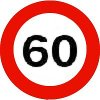
\includegraphics[width=1cm]{./imagenes/6.jpg} \\
      \hline

      Identificador: & 1 & 2 & 3 & 4 & 5 & 6 \\
      \hline
      Figura externa:& 8 & 9 & 9 & 9 & 9 & 9 \\     
      \hline
      Perímetro:& 506.877 & 1025.25 & 1565.18 & 1971.43 & 2510.69 & 2979.51 \\
      \hline 
      Área: & 8384.5 & 12774.5 & 17323.5 & 21771 & 26734 & 30611.5 \\ 
      \hline
      Número de vértices: & 39 & 77 & 125 & 156 & 197 & 236 \\ 
      \hline
      Piezas interiores: & 4 & 2 & 2 & 2 & 2 & 2 \\
      \hline
    \end{tabular}
  \end{center}
  \caption{Tabla con los datos extraídos para algunas de las clases (señales) a identificar.}
  \label{table:tabla-modelos}
\end{table}

Por tanto la matriz de modelos obtenida queda de la siguiente manera:\\

\[
 M =
 \begin{pmatrix}
  1 & 2 & 3 & 4 & 5 & 6 & 7 & 8 & \cdots\\
  8 & 9 & 9 & 9 & 9 & 9 & 9 & 9 & \cdots\\     
  506.877 & 1025.25 & 1565.18 & 1971.43 & 2510.69 & 2979.51 & 3406.49 & 3828.48 & \cdots\\
  4001 8384.5 & 12774.5 & 17323.5 & 21771 & 26734 & 30611.5 & 35896.5 & 40857 & \cdots\\ 
  39 & 77 & 125 & 156 & 197 & 236 & 264 & 299 & \cdots\\
  4 & 2 & 2 & 2 & 2 & 2 & 2 & 2 & \cdots\\
 \end{pmatrix}
\]

\subsection{Clasificación}

Para la clasificación se ha empleado un algoritmo denominado \emph{el vecino más cercano} haciendo uso de los datos extraídos del objeto desconocido y de la matriz modelos obtenida durante la etapa de entrenamiento. \\

Para proceder a la extracción de los datos del objeto desconocido se ha realizado los mismos pasos que durante la etapa de entrenamiento solo que aplicándose a una imagen de entrada, en lugar de aplicarse con las imágenes reservadas para entrenar el sistema.\\

Una vez obtenido el vector de característica del elemento desconocido, se realiza la llamada al algoritmo del vecino más cercano recibiendo la matriz de modelos previamente obtenida de la etapa de entrenamiento junto con el vector de característica del objeto a identificar. La figura \ref{math:vector-columna} muestra una imagen representativa de un vector característica del que cuya clase de pertenencia es desconocida:\\

\begin{figure}[H]
  \begin{center}
    \[
    Vdesconocido =
    \begin{pmatrix}
      8\\     
      502.237 \\
      4022 \\ 
      34 \\
      4 
      \nocite{}
    \end{pmatrix}
    \]
  \end{center}
  \caption{Vector de características de un elemento desconocido.}
  \label{math:vector-columna}
\end{figure}

Como podemos apreciar, el objeto desconocido (del que no se conoce su clase) es representado por una matriz columna. A continuación se calcula la distancia euclídea entre cada uno de los vectores columnas integrantes de la matriz modelos y el vector desconocido, seleccionándose el ejemplo más cercano. El nuevo ejemplo es clasificado con la clase que pertenece el vector seleccionado dentro de la matriz modelos.\\

Este método supone que el vecino más cercano nos dé la mejor clasificación y esto se hace utilizando todos los atributos; el problema de dicha suposición es que es posible que se tengan muchos atributos irrelevantes que dominen sobre la clasificación: dos atributos relevantes perderían peso entre otros irrelevantes.\\

A continuación se muestra la fórmula para el cálculo de la distancia euclídea, definida como la raíz cuadrada de las sumas de las diferencias de las componentes al cuadrado:\\

\begin{figure}[H]
  \begin{center}
    \[
    d(x_{i},y_{j}) = \sqrt{\sum_{r=1}^p (x_{ir}-x_{jr})^2}
    \nocite{}
    \]
  \end{center}
  \label{eq:dist-euclid}
  \caption{Fórmula para el cálculo de la distancia euclídea, definida como la raíz cuadrada de las sumas de las diferencias de cada una de las componentes del vector al cuadrado.}
\end{figure}

A continuación se muestra el código realizado para la clasificación utilizando el algoritmo del vecino más cercano:\\

\underline{Aplicación del vecino más cercano}\\
\begin{Verbatim}[commandchars=\\\{\}]
\PY{k+kt}{int} \PY{n}{Clasificador}\PY{p}{(}\PY{n}{CvMat} \PY{n}{DatosEntrenamiento}\PY{p}{,} \PY{n}{CvMat} \PY{n}{DatosCandidato}\PY{p}{)}\PY{p}{\PYZob{}}

  \PY{c+c1}{// Aplicación del algoritmo KNN.}
  
  \PY{k}{const} \PY{k+kt}{int} \PY{n}{K} \PY{o}{=} \PY{l+m+mi}{1}\PY{p}{;} \PY{c+c1}{// Se fija valor de K. (K=1, vecino más cercano).}
  \PY{k+kt}{int} \PY{n}{solucion}\PY{p}{;}    \PY{c+c1}{// Solución}
  
  \PY{c+c1}{// Se crea e inicializa el vector de clases, cada elemento columna de }
  \PY{c+c1}{// DatosEntrenamiento es una clase}
  
  \PY{k+kt}{int} \PY{n}{clases}\PY{p}{[}\PY{n}{elementos}\PY{p}{]}\PY{p}{;}	
  \PY{n}{CvMat}  \PY{n}{Clases} \PY{o}{=} \PY{n}{cvMat}\PY{p}{(}\PY{n}{elementos}\PY{p}{,}\PY{l+m+mi}{1}\PY{p}{,} \PY{n}{CV\PYZus{}32FC1}\PY{p}{,}\PY{n}{clases}\PY{p}{)}\PY{p}{;}
  
  \PY{k}{for} \PY{p}{(}\PY{k+kt}{int} \PY{n}{a}\PY{o}{=}\PY{l+m+mi}{0}\PY{p}{;}\PY{n}{a}\PY{o}{<}\PY{n}{DatosEntrenamiento}\PY{p}{.}\PY{n}{rows}\PY{p}{;}\PY{n}{a}\PY{o}{+}\PY{o}{+}\PY{p}{)}\PY{p}{\PYZob{}}
    \PY{k}{for} \PY{p}{(}\PY{k+kt}{int} \PY{n}{b}\PY{o}{=}\PY{l+m+mi}{0}\PY{p}{;}\PY{n}{b}\PY{o}{<}\PY{n}{Clases}\PY{p}{.}\PY{n}{cols}\PY{p}{;}\PY{n}{b}\PY{o}{+}\PY{o}{+}\PY{p}{)}\PY{p}{\PYZob{}}
      \PY{c+c1}{// Se añaden los identificadores.}
      \PY{n}{cvSetReal2D}\PY{p}{(}\PY{o}{&}\PY{n}{Clases}\PY{p}{,}\PY{n}{a}\PY{p}{,}\PY{n}{b}\PY{p}{,}\PY{n}{a}\PY{o}{+}\PY{l+m+mi}{1}\PY{p}{)}\PY{p}{;}
    \PY{p}{\PYZcb{}}
  \PY{p}{\PYZcb{}}
  
  \PY{c+c1}{// Se crea el clasificador.}
  \PY{n}{CvKNearest} \PY{n}{knn}\PY{p}{(} \PY{o}{&}\PY{n}{DatosEntrenamiento}\PY{p}{,} \PY{o}{&}\PY{n}{Clases}\PY{p}{,} \PY{l+m+mi}{0}\PY{p}{,} \PY{n+nb}{false}\PY{p}{,} \PY{n}{K} \PY{p}{)}\PY{p}{;}
  \PY{n}{CvMat}\PY{o}{*} \PY{n}{nearests} \PY{o}{=} \PY{n}{cvCreateMat}\PY{p}{(} \PY{l+m+mi}{1}\PY{p}{,} \PY{n}{K}\PY{p}{,} \PY{n}{CV\PYZus{}32FC1}\PY{p}{)}\PY{p}{;}
  
  \PY{c+c1}{// Se estima el vecino más cercano.}
  \PY{n}{solucion} \PY{o}{=} \PY{n}{knn}\PY{p}{.}\PY{n}{find\PYZus{}nearest}\PY{p}{(}\PY{o}{&}\PY{n}{DatosCandidato}\PY{p}{,}\PY{n}{K}\PY{p}{,}\PY{l+m+mi}{0}\PY{p}{,}\PY{l+m+mi}{0}\PY{p}{,}\PY{n}{nearests}\PY{p}{,}\PY{l+m+mi}{0}\PY{p}{)}\PY{p}{;}
   
  \PY{c+c1}{// Se devuelve el resultado.}
  \PY{k}{return}  \PY{n}{solucion}\PY{p}{;}
\PY{p}{\PYZcb{}}
\end{Verbatim}



\subsection{Problemas detectados}

Los problemas que han llevado a cabo el rechazo de este segundo prototipo han sido los siguientes:

\begin{itemize}

\item Los datos obtenidos durante la extracción de características tales como área, perímetro, número de vértices, número de objetos interiores de la señal, entre otros, no resultaban determinantes y excluyentes a la hora de realizar la clasificación proporcionando un alto número de errores cuando el objetivo es elaborar un sistema lo más fiable y eficiente posible.

\item Como punto positivo, se ha comprobado que el algoritmo de los k-vecinos presenta un funcionamiento más adecuado a las características exigibles del proyecto trabajando con los datos de entrada adecuados ya que proporciona una buena relación entre tiempo computacional y efectividad. Por otro lado, el algoritmo presenta la posibilidad de identificación de más de una clase ya que como entrada es capaz de recibir datos de distintas clases a identificar como no ocurría con la comparación de plantillas . Por estas razones se ha considerado adecuado continuar el desarrollo del siguiente prototipo haciendo uso del algoritmo K-vecinos más cercanos cambiando los datos de entrada por otro conjunto de datos que hagan mejorar su funcionamiento.

\end{itemize}

\section{Tercer y último prototipo}

Dado que el prototipo anterior presentaba una baja relación de aciertos, y observando la idoneidad de continuar con el algoritmo del k-vecinos más cercano con valores de K = 1. Se ha optado por continuar con la misma técnica de clasificación cambiando los datos integrantes de la matriz de modelos por unos más representativos.

\subsection{Extracción de características}

Para la extracción de las características necesarias para la creación de la matriz de modelos por parte del algoritmo de entrenamiento han sido necesarias una serie de etapas que se describen en las sucesivas secciones.

\subsubsection{Segmentación por color}

Como etapa inicial, se ha seguido con la metodología empleada en el segundo prototipo utilizando, del igual modo, una segmentación por color aplicando el modelo de color HSV. La única salvedad radica en que en esta ocasión se han añadido los valores necesarios para filtrar las tonalidades azules. En la sección \ref{sec:color-HSV}, referente al segundo prototipo, se describe al detalle la metodología seguida.

\subsubsection{Obtención de datos representativos}

En esta ocasión se ha procedido extraer de forma separada los elementos interiores de una señal de tráfico, para ello a cada objeto identificado tras la selección de color se le aplica un relleno y se extrae mediante máscaras el objeto de la imagen original siguiendo la misma metodología que en el primer prototipo. Ver sección \ref{sec:extraccion-objetos} para consultar el proceso detalladamente.\\

Posteriormente, la imagen obtenida con el objeto candidato es pasada a escala de grises y se identificaban los contornos. Cada uno de los contornos detectados se corresponden con un elemento interno de la posible señal de tráfico. Los contornos son dibujados rellenando sus huecos vacíos con el fin de eliminar los contornos interiores.\\

Cada elemento es a su vez extraído en una nueva imagen donde es redimensionado a un tamaño fijado y dispuesto en un vector columna, dicho vector columna es utilizado para ser agregado a la matriz modelos. La figura \ref{fig:pasos-prototipo3} muestra una representación del proceso seguido. \\


\begin{figure}[H]
  \begin{center}
      \begin{tabular}{ccccc p{3cm}p{3cm}p{3cm}p{1cm}}
        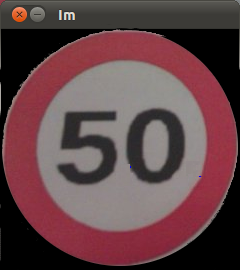
\includegraphics[width=3cm]{./imagenes/mascara/mascara3.png} &  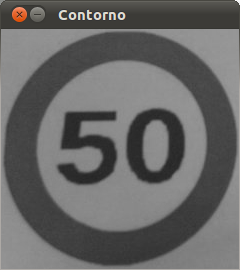
\includegraphics[width=3cm]{./imagenes/prototipo3/Contornogris.png} &  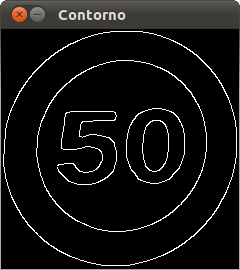
\includegraphics[width=3cm]{./imagenes/prototipo3/contorno.png} &  \includegraphics[width=0.95cm]{./imagenes/prototipo3/elementos2.png} \\
        {(\emph{a})} & {(\emph{b})} & {(\emph{c})} & {(\emph{d})} \\
      \end{tabular}
    \caption{Proceso seguido para la extracción de los objetos interiores de una señal.}
    \label{fig:pasos-prototipo3}
  \end{center}
\end{figure}

En la imagen (\emph{d}) de la figura \ref{fig:pasos-prototipo3} se visualiza el elemento 0 y el 5 por separado. Ambas matrices representativas de las imágenes, junto con las del resto de elementos a identificar, son dispuestas en vectores columnas y agregadas a la matriz de modelos junto con su identificador, se ha empleado como identificador un carácter numérico para el caso de los números, caracteres alfabéticos para las letras implicadas como las existentes en la señal de Stop y otros caracteres para el resto de elementos como las flechas indicadoras de dirección. Ver figuras \ref{fig:representacion-cinco} y \ref{fig:representacion-columna-cinco}.\\

\begin{figure}[H]
  \begin{center}
    \[
    V_1 =
    \begin{pmatrix}
      1 & 1 & 1 & 1 & 1 & 1 & 1 & 1\\
      1 & 1 & 1 & 1 & 1 & 1 & 1 & 1\\
      1 & 1 & 0 & 0 & 0 & 0 & 0 & 0\\ 
      1 & 1 & 0 & 0 & 0 & 0 & 0 & 0\\ 
      1 & 1 & 1 & 1 & 1 & 1 & 1 & 1\\    
      1 & 1 & 1 & 1 & 1 & 1 & 1 & 1\\
      0 & 0 & 0 & 0 & 0 & 0 & 1 & 1\\ 
      0 & 0 & 0 & 0 & 0 & 0 & 1 & 1\\
      1 & 1 & 1 & 1 & 1 & 1 & 1 & 1\\
      1 & 1 & 1 & 1 & 1 & 1 & 1 & 1\\
    \end{pmatrix}
    \]
    \caption{Representación del número cinco en una matriz.}
    \label{fig:representacion-cinco}
  \end{center}
\end{figure}

\begin{figure}[H]
  \begin{center}
    \[
    V_2 =
    \begin{pmatrix}
      5 \\ 1 \\ 1 \\ 1 \\ 1 \\ 1 \\ 1 \\ 1 \\ 1\\ \vdots\\ 1 \\ 1 \\ 1
    \end{pmatrix}
    \]
    \caption{Resultado de la transformación de la matriz $V_1$ en vector columna añadiendo las diferentes columnas de $V_1$ sucesivamente una bajo la otra en $V_2$. El vector resultante posee en la primera posición el identificador de la clase, en el caso mostrado el carácter ``5''.}
    \label{fig:representacion-columna-cinco}
  \end{center}
\end{figure}

\subsection{Clasificación}

Para proceder con la clasificación, previamente la matriz modelos es cargada de un fichero donde se encuentra almacenada.\\

Antes de realizar la clasificación hay que procesar la imagen de entrada del mismo modo que se ha realizado durante la etapa de entrenamiento. Cada elemento existente dentro de una figura circular roja es extraído y dispuesto en un vector columna para ser clasificado mediante el algoritmo del vecino más cercano. Supongamos la señal de 50km/h. Sus elementos interiores son el carácter ``5'' y el carácter ``0''. Por tanto, si se aplica el algoritmo del vecino más cercano nos producirá como salida en la primera llamada un ``5'' y en la segunda un ``0''. Dado que ambos elementos se encuentran dentro de una circunferencia de color rojo, se determina que el objeto procesado se trata de la señal de 50km/h. Ver figura \ref{fig:salida-protot3}. \\

\begin{figure}[H]
  \begin{center}
        \includegraphics[width=3cm]{./imagenes/prototipo3/salida3.png}
  \end{center}
    \caption{Identificación de los elementos interiores de la señal, el valor ``5'' y el valor ``0'', determinándose el objeto como una señal de 50 km/h.}
    \label{fig:salida-protot3}
\end{figure}

El algoritmo de clasificación empleado ha sido el mismo que el utilizado en el prototipo anterior con la salvedad de que en esta ocasión se rechazan aquellos valores de salida cuya distancia supera un determinado umbral. Con esta modificación los elementos serán clasificados cuando su grado de parentesco es elevado y no con la clase con la que más se le parece aunque sea un objeto totalmente diferente.\\

A continuación se muestra el código modificado:\\

\underline{Algoritmo del vecino más cercano modificado para la obtención de las distancias}\\

\begin{Verbatim}[commandchars=\\\{\}]
\PY{k+kt}{int} \PY{n}{Clasificador}\PY{p}{(}\PY{n}{CvMat} \PY{n}{DatosEntrenamiento}\PY{p}{,} \PY{n}{CvMat} \PY{n}{DatosCandidato}\PY{p}{)}\PY{p}{\PYZob{}}

  \PY{c+c1}{// Aplicación del algoritmo KNN.}
  
  \PY{k}{const} \PY{k+kt}{int} \PY{n}{K} \PY{o}{=} \PY{l+m+mi}{1}\PY{p}{;} \PY{c+c1}{// Se fija valor de K. (K=1, vecino más cercano).}
  \PY{k+kt}{int} \PY{n}{solucion}\PY{p}{;}    \PY{c+c1}{// Solución}
  \PY{k+kt}{int} \PY{n}{umbral\PYZus{}minimo} \PY{o}{=} \PY{l+m+mi}{10000}\PY{p}{;} \PY{c+c1}{// Grado de semejanza exigido.}

  \PY{c+c1}{// Vector donde se almacenarán las distancias.}
  \PY{n}{CvMat}\PY{o}{*} \PY{n}{distancias} \PY{o}{=} \PY{n}{cvCreateMat}\PY{p}{(}\PY{l+m+mi}{1}\PY{p}{,}\PY{n}{K}\PY{p}{,}\PY{n}{CV\PYZus{}32FC1}\PY{p}{)}\PY{p}{;}
 
  
  \PY{c+c1}{// Se crea e inicializa el vector de clases, cada elemento columna de }
  \PY{c+c1}{// DatosEntrenamiento es una clase.}
 
  \PY{k+kt}{int} \PY{n}{clases}\PY{p}{[}\PY{n}{elementos}\PY{p}{]}\PY{p}{;}	
  \PY{n}{CvMat}  \PY{n}{Clases} \PY{o}{=} \PY{n}{cvMat}\PY{p}{(}\PY{n}{elementos}\PY{p}{,}\PY{l+m+mi}{1}\PY{p}{,} \PY{n}{CV\PYZus{}32FC1}\PY{p}{,}\PY{n}{clases}\PY{p}{)}\PY{p}{;}
  
  \PY{k}{for} \PY{p}{(}\PY{k+kt}{int} \PY{n}{a}\PY{o}{=}\PY{l+m+mi}{0}\PY{p}{;}\PY{n}{a}\PY{o}{<}\PY{n}{DatosEntrenamiento}\PY{p}{.}\PY{n}{rows}\PY{p}{;}\PY{n}{a}\PY{o}{+}\PY{o}{+}\PY{p}{)}\PY{p}{\PYZob{}}
    \PY{k}{for} \PY{p}{(}\PY{k+kt}{int} \PY{n}{b}\PY{o}{=}\PY{l+m+mi}{0}\PY{p}{;}\PY{n}{b}\PY{o}{<}\PY{n}{Clases}\PY{p}{.}\PY{n}{cols}\PY{p}{;}\PY{n}{b}\PY{o}{+}\PY{o}{+}\PY{p}{)}\PY{p}{\PYZob{}}
      \PY{c+c1}{// Se añaden los identificadores.}
      \PY{n}{cvSetReal2D}\PY{p}{(}\PY{o}{&}\PY{n}{Clases}\PY{p}{,}\PY{n}{a}\PY{p}{,}\PY{n}{b}\PY{p}{,}\PY{n}{a}\PY{o}{+}\PY{l+m+mi}{1}\PY{p}{)}\PY{p}{;}
    \PY{p}{\PYZcb{}}
  \PY{p}{\PYZcb{}}
  
  \PY{c+c1}{// Se crea el clasificador.}
  \PY{n}{CvKNearest} \PY{n}{knn}\PY{p}{(} \PY{o}{&}\PY{n}{DatosEntrenamiento}\PY{p}{,} \PY{o}{&}\PY{n}{Clases}\PY{p}{,} \PY{l+m+mi}{0}\PY{p}{,} \PY{n+nb}{false}\PY{p}{,} \PY{n}{K} \PY{p}{)}\PY{p}{;}
  \PY{n}{CvMat}\PY{o}{*} \PY{n}{nearests} \PY{o}{=} \PY{n}{cvCreateMat}\PY{p}{(} \PY{l+m+mi}{1}\PY{p}{,} \PY{n}{K}\PY{p}{,} \PY{n}{CV\PYZus{}32FC1}\PY{p}{)}\PY{p}{;}
  
  \PY{c+c1}{// Se estima el vecino más cercano.}
  \PY{n}{solucion} \PY{o}{=} \PY{n}{knn}\PY{p}{.}\PY{n}{find\PYZus{}nearest}\PY{p}{(}\PY{n}{elemento\PYZus{}analisis}\PY{p}{,}\PY{n}{K}\PY{p}{,}\PY{l+m+mi}{0}\PY{p}{,}\PY{l+m+mi}{0}\PY{p}{,}\PY{n}{nearests}\PY{p}{,}\PY{n}{distancias}\PY{p}{)}\PY{p}{;}
   
  \PY{c+c1}{//Si hay bastante semejanza, aceptamos como válido. }
  \PY{k}{if} \PY{p}{(}\PY{n}{cvGetReal2D}\PY{p}{(}\PY{n}{distancias}\PY{p}{,}\PY{l+m+mi}{0}\PY{p}{,}\PY{l+m+mi}{0}\PY{p}{)} \PY{o}{<} \PY{n}{umbral\PYZus{}minimo}\PY{p}{)}\PY{p}{\PYZob{}} 
	\PY{k}{return} \PY{n}{solucion}\PY{p}{;}
  \PY{p}{\PYZcb{}}
  \PY{c+c1}{// Si no se devuelve cero.}
  \PY{k}{return}  \PY{l+m+mi}{0}\PY{p}{;}
\PY{p}{\PYZcb{}}
\end{Verbatim}





% Este archivo es parte de la memoria del proyecto fin de carrera
% de Manuel López Urbina. Protegida bajo la licencia GFDL.
% Para más información, la licencia completa viene incluida en el
% fichero fdl-1.3.tex

% Copyright (C) 2012 Manuel López Urbina

\chapter{Software de control}
\label{chap:software-de-control}

En presente capítulo contiene información relativa a las herramientas software utilizadas y desarrolladas para la realización de la comunicación con el vehículo ordenando acciones como movimientos, modificación de velocidad, entre otros. Todo ello desde el ordenador por parte del usuario.\\

Cabe recordar que la aplicación consta de dos modos de funcionamiento; un modo automático donde los movimientos son realizados a partir de los elementos visionados por la cámara, y un segundo modo donde el vehículo es manejable por el usuario. En este tema de desarrollan ambos aspectos.\\

Para el control del vehículo se ha utilizado un software denominado \emph{Surveyor Robot Software} \footnote{Para la descarga de código fuente visite el siguiente enlace \url{{http://agents.sci.brooklyn.cuny.edu/robotics.edu/bcsoftware.php}}.}, el cual ha sido desarrollado por John Cummins junto con los agentes de laboratorio de la Universidad de Brooklyn con la asistencia de M.P. Azhar, y la supervisión del profesor Sklar empleando el lenguaje de programación C++. El código está liberado bajo Copyleft.\\

El código \emph{Surveyor robot software} ha sido ligeramente modificado para adaptarlo a las necesidades del proyecto, la principal modificación añadida ha sido la de añadir un método para permitir la conexión y desconexión con el vehículo. Permitiendo al usuario desconectar y reconectar a su antojo.

\section{Control por parte del usuario}

Lo interesante era proporcionar una serie de mecanismos que permitiera mantener un control del vehículo de una manera cómoda y eficaz para el usuario. Los elementos proporcionados para realizar el control del vehículo son el uso del teclado del ordenador y un gamepad.

\subsection{Control desde teclado}

Los movimientos clásicos del vehículo, avance, retroceso y giros, han sido ordenados mediante el uso de las teclas de dirección. Para las capturas de los eventos desde el teclado se han utilizado las herramientas proporcionadas por la biblioteca Qt.\\

De este modo, el vehículo, al presionar la tecla de avance, comenzaba a andar, pero no se detenía hasta nueva orden haciendo incómodo su manejo. Como solución al problema se optó por capturar el evento de ``soltado'' de tecla para, en ese instante, mandar una orden de detención de tal manera que el vehículo avance sólo y exclusivamente mientras se encuentra la tecla pulsada.\\

Por otro lado, el robot SRV-1, al tratarse de un vehículo tipo tanque, presenta la particularidad de poder controlar las velocidades de movimiento de los motores de un mismo lateral por igual permitiendo la realización de giros. Como consecuencia de lo anterior, si se aplica una velocidad levemente inferior en un lateral que en el otro el vehículo realizará un giro muy abierto. De modo contrario, si detenemos por completo los motores de un lado, el giro producido será de pequeña amplitud. Esta circunstancia permite que desde las flechas de teclado no podamos controlar tal efecto, puesto que los giros serán siempre iguales, que para el caso de las teclas de dirección será únicamente moviendo los motores de un lateral.\\

\begin{figure}[H]
  \begin{center}
    \includegraphics[scale=0.5]{quad-base.jpg}
  \end{center}
  \caption{Visualización del chasis del robot y su sistema de desplazamiento tipo tanque.}
  \label{fig:quad-base}
\end{figure}

 Para permitir realizar ambos tipos de giros se pensó en capturar combinaciones de teclas, de tal modo que si se presiona la tecla ``derecha'', el vehículo realice un giro cerrado y si se presiona la tecla ``arriba'' más ``derecha'', el giro será de mayor amplitud. Los diferentes movimientos existentes en el vehículo quedan descritos en la sección \ref{sec:uso-teclado} del manual.\\

Para su realización, Qt no dispone de los elementos necesarios para capturar combinaciones de teclas, solamente es posible con las teclas ``Shift'', ``Ctrl'',`` Alt'' y ``Meta''.\\

Como solución al problema de la captura de eventos múltiples se implementó un buffer donde se almacenaba un identificador de las dos últimas teclas pulsadas, eliminándose un identificador del buffer en el momento en que la tecla sea soltada. De ese modo tras la captura de un evento, se analizaba el estado del buffer y se determinaba la orden de movimiento a realizar. Obteniendo los movimientos descritos en la sección \ref{sec:uso-teclado} del manual.\\

En la siguiente imagen podemos ver una representación gráfica del comportamiento del buffer de control del vehículo:\\

\begin{figure}[H]
  \begin{center}
    \includegraphics[scale=0.8]{buffer-teclado2.png}
  \end{center}
  \caption{Representación del funcionamiento del buffer creado para la captura de eventos múltiples.}
  \label{fig:buffer-teclado}
\end{figure}


\subsection{Control mediante gamepad}

Para hacer más cómodo, aún si cabe, el manejo del vehículo, se decidió incorporar un mando o gamepad, para ello ha sido necesaria la utilización de la biblioteca SDL con el fin de detectar el dispositivo y capturar los eventos correspondientes no presentando dificultades destacables. Para ver los controles fijados vea sección \ref{sec:convencion-gamepad} de la guía de usuario.

\section{Control automático}

Para dotar al vehículo de un sistema de conducción autónoma se han diseñado una serie de respuestas automáticas ordenadas cuando una determinada señal es detectada. En esta sección se describen cada una de ellas.\\

Entre el conjunto de señales de tráfico reconocibles por el sistema disponemos de las indicadoras de velocidad máxima. Estas señales detectables varían desde los 20 hasta los 100 km/h. Cuando una determinada velocidad es detectada, ésta debe ser asignada al vehículo con la finalidad de realizar los movimientos de una manera proporcional a la velocidad indicadora de la señal reconocida. \\

La biblioteca \emph{Surveyor Robot Software} permite ajustar las velocidades de movimiento del vehículo en una escala desde el 0 hasta el 100. Por tanto, si la señal de tráfico detectada se corresponde con la de 50km/h, se asigna al vehículo un valor de velocidad de 50.\\

En el momento de la detección de la señal de Stop, se ordena su detención manteniéndose intacto el valor de velocidad que se encuentra en ese momento fijado.\\

Para las señales correspondientes a las indicadoras de dirección obligatoria (flechas), se efectúa un giro de manera automática. En la sección \ref{sec:operaciones-automatizadas} del manual se muestra al detalle los diferentes movimientos realizados para cada señal de tráfico detectada.\\

Por otro lado, cuando una señal es detectada, la orden automatizada es enviada al vehículo una sola vez de tal modo que si en el entorno apareciese más adelante la misma señal reconocida anteriormente, ésta no se volverá a realizar. En definitiva, no se reconoce la misma señal de tráfico dos veces seguidas. \\

\begin{figure}[H]
  \begin{center}
    \includegraphics[scale=0.8]{circuito.jpg}
  \end{center}
  \caption{Fotografía de un circuito realizable por el vehículo .}
  \label{fig:circuito}
\end{figure}


A continuación se muestra el código realizado para la realización de los movimientos autónomos. En ella se analiza un vector para comprobar si contiene los identificadores de las clases de aquellos objetos que se correspondan con una señal. Por ejemplo, si el vector contiene los identificadores ``2'' y ``0'' determinamos que el elemento detectado es una señal de 20 km/h.\\

\underline{Código para el control automatizado del vehículo}
\begin{Verbatim}[commandchars=\\\{\}]
\PY{k+kt}{int}  \PY{n}{MainWindow}\PY{o}{:}\PY{o}{:}\PY{n}{accion\PYZus{}SVR}\PY{p}{(}\PY{n}{std}\PY{o}{:}\PY{o}{:}\PY{n}{vector}\PY{o}{<}\PY{k+kt}{char}\PY{o}{>} \PY{o}{&}\PY{n}{v}\PY{p}{)}\PY{p}{\PYZob{}}


    \PY{c+c1}{// 100 km/h}
    \PY{k}{if} \PY{p}{(}\PY{p}{(}\PY{n}{std}\PY{o}{:}\PY{o}{:}\PY{n}{find}\PY{p}{(}\PY{n}{v}\PY{p}{.}\PY{n}{begin}\PY{p}{(}\PY{p}{)}\PY{p}{,} \PY{n}{v}\PY{p}{.}\PY{n}{end}\PY{p}{(}\PY{p}{)}\PY{p}{,}\PY{l+s+sc}{'1'}\PY{p}{)}\PY{o}{!}\PY{o}{=} \PY{n}{v}\PY{p}{.}\PY{n}{end}\PY{p}{(}\PY{p}{)}\PY{p}{)} \PY{o}{&}\PY{o}{&}
        \PY{p}{(}\PY{n}{std}\PY{o}{:}\PY{o}{:}\PY{n}{find}\PY{p}{(}\PY{n}{v}\PY{p}{.}\PY{n}{begin}\PY{p}{(}\PY{p}{)}\PY{p}{,} \PY{n}{v}\PY{p}{.}\PY{n}{end}\PY{p}{(}\PY{p}{)}\PY{p}{,}\PY{l+s+sc}{'0'}\PY{p}{)} \PY{o}{!}\PY{o}{=} \PY{n}{v}\PY{p}{.}\PY{n}{end}\PY{p}{(}\PY{p}{)}\PY{p}{)}\PY{p}{)}\PY{p}{\PYZob{}}

        \PY{c+c1}{// Se elimina un '0'.}
        \PY{n}{std}\PY{o}{:}\PY{o}{:}\PY{n}{vector}\PY{o}{<}\PY{k+kt}{char}\PY{o}{>}\PY{o}{:}\PY{o}{:}\PY{n}{iterator} \PY{n}{pos} \PY{o}{=} \PY{n}{std}\PY{o}{:}\PY{o}{:}\PY{n}{find}\PY{p}{(}\PY{n}{v}\PY{p}{.}\PY{n}{begin}\PY{p}{(}\PY{p}{)}\PY{p}{,} \PY{n}{v}\PY{p}{.}\PY{n}{end}\PY{p}{(}\PY{p}{)}\PY{p}{,}\PY{l+s+sc}{'0'}\PY{p}{)}\PY{p}{;}
        \PY{n}{v}\PY{p}{.}\PY{n}{erase}\PY{p}{(}\PY{n}{pos}\PY{p}{)}\PY{p}{;}

        \PY{c+c1}{// Si existe otro cero...}
        \PY{k}{if}\PY{p}{(}\PY{n}{std}\PY{o}{:}\PY{o}{:}\PY{n}{find}\PY{p}{(}\PY{n}{v}\PY{p}{.}\PY{n}{begin}\PY{p}{(}\PY{p}{)}\PY{p}{,} \PY{n}{v}\PY{p}{.}\PY{n}{end}\PY{p}{(}\PY{p}{)}\PY{p}{,}\PY{l+s+sc}{'0'}\PY{p}{)}\PY{o}{!}\PY{o}{=} \PY{n}{v}\PY{p}{.}\PY{n}{end}\PY{p}{(}\PY{p}{)}\PY{p}{)}\PY{p}{\PYZob{}}

            \PY{c+c1}{// 100 km/h}
            \PY{k}{if}\PY{p}{(}\PY{n}{conectado} \PY{o}{&}\PY{o}{&} \PY{n}{ui}\PY{o}{-}\PY{o}{>}\PY{n}{checkBox\PYZus{}2}\PY{o}{-}\PY{o}{>}\PY{n}{isChecked}\PY{p}{(}\PY{p}{)} \PY{o}{&}\PY{o}{&} \PY{n}{ultima\PYZus{}senial} \PY{o}{!}\PY{o}{=} \PY{l+m+mi}{10}\PY{p}{)}\PY{p}{\PYZob{}}
                \PY{n}{ultima\PYZus{}senial} \PY{o}{=} \PY{l+m+mi}{10}\PY{p}{;}
                \PY{n}{robot}\PY{p}{.}\PY{n}{move}\PY{p}{(}\PY{n}{STOP}\PY{p}{)}\PY{p}{;}
                \PY{n}{this}\PY{o}{-}\PY{o}{>}\PY{n}{velocidad} \PY{o}{=} \PY{l+m+mi}{100}\PY{p}{;}
                \PY{n}{robot}\PY{p}{.}\PY{n}{drive}\PY{p}{(}\PY{n}{this}\PY{o}{-}\PY{o}{>}\PY{n}{velocidad}\PY{p}{,}\PY{n}{this}\PY{o}{-}\PY{o}{>}\PY{n}{velocidad}\PY{p}{)}\PY{p}{;}
            \PY{p}{\PYZcb{}}
            \PY{c+c1}{//Mostrar señal detectada}
            \PY{n}{mostrar\PYZus{}senial\PYZus{}detectada}\PY{p}{(}\PY{l+s}{"}\PY{l+s}{10.jpg}\PY{l+s}{"}\PY{p}{)}\PY{p}{;}

            \PY{k}{return} \PY{l+m+mi}{0}\PY{p}{;}
        \PY{p}{\PYZcb{}}
    \PY{p}{\PYZcb{}}


    \PY{c+c1}{// 20 km/h}
    \PY{k}{if} \PY{p}{(}\PY{p}{(}\PY{n}{std}\PY{o}{:}\PY{o}{:}\PY{n}{find}\PY{p}{(}\PY{n}{v}\PY{p}{.}\PY{n}{begin}\PY{p}{(}\PY{p}{)}\PY{p}{,} \PY{n}{v}\PY{p}{.}\PY{n}{end}\PY{p}{(}\PY{p}{)}\PY{p}{,}\PY{l+s+sc}{'2'}\PY{p}{)} \PY{o}{!}\PY{o}{=} \PY{n}{v}\PY{p}{.}\PY{n}{end}\PY{p}{(}\PY{p}{)}\PY{p}{)} \PY{o}{&}\PY{o}{&} 
        \PY{p}{(}\PY{n}{std}\PY{o}{:}\PY{o}{:}\PY{n}{find}\PY{p}{(}\PY{n}{v}\PY{p}{.}\PY{n}{begin}\PY{p}{(}\PY{p}{)}\PY{p}{,} \PY{n}{v}\PY{p}{.}\PY{n}{end}\PY{p}{(}\PY{p}{)}\PY{p}{,}\PY{l+s+sc}{'0'}\PY{p}{)} \PY{o}{!}\PY{o}{=} \PY{n}{v}\PY{p}{.}\PY{n}{end}\PY{p}{(}\PY{p}{)}\PY{p}{)}\PY{p}{)}\PY{p}{\PYZob{}}

        \PY{k}{if}\PY{p}{(}\PY{n}{conectado} \PY{o}{&}\PY{o}{&} \PY{n}{ui}\PY{o}{-}\PY{o}{>}\PY{n}{checkBox\PYZus{}2}\PY{o}{-}\PY{o}{>}\PY{n}{isChecked}\PY{p}{(}\PY{p}{)} \PY{o}{&}\PY{o}{&} \PY{n}{ultima\PYZus{}senial} \PY{o}{!}\PY{o}{=} \PY{l+m+mi}{2}\PY{p}{)}\PY{p}{\PYZob{}}
            \PY{n}{ultima\PYZus{}senial} \PY{o}{=} \PY{l+m+mi}{2}\PY{p}{;}
            \PY{n}{robot}\PY{p}{.}\PY{n}{move}\PY{p}{(}\PY{n}{STOP}\PY{p}{)}\PY{p}{;}
            \PY{n}{this}\PY{o}{-}\PY{o}{>}\PY{n}{velocidad} \PY{o}{=} \PY{l+m+mi}{20}\PY{p}{;}
            \PY{n}{robot}\PY{p}{.}\PY{n}{drive}\PY{p}{(}\PY{n}{this}\PY{o}{-}\PY{o}{>}\PY{n}{velocidad}\PY{p}{,}\PY{n}{this}\PY{o}{-}\PY{o}{>}\PY{n}{velocidad}\PY{p}{)}\PY{p}{;}
        \PY{p}{\PYZcb{}}
        \PY{c+c1}{//Mostrar señal detectada}
        \PY{n}{mostrar\PYZus{}senial\PYZus{}detectada}\PY{p}{(}\PY{l+s}{"}\PY{l+s}{2.jpg}\PY{l+s}{"}\PY{p}{)}\PY{p}{;}
        \PY{k}{return} \PY{l+m+mi}{0}\PY{p}{;}
    \PY{p}{\PYZcb{}}

    \PY{c+c1}{// 30 km/h}
    \PY{k}{if} \PY{p}{(}\PY{p}{(}\PY{n}{std}\PY{o}{:}\PY{o}{:}\PY{n}{find}\PY{p}{(}\PY{n}{v}\PY{p}{.}\PY{n}{begin}\PY{p}{(}\PY{p}{)}\PY{p}{,} \PY{n}{v}\PY{p}{.}\PY{n}{end}\PY{p}{(}\PY{p}{)}\PY{p}{,}\PY{l+s+sc}{'3'}\PY{p}{)} \PY{o}{!}\PY{o}{=} \PY{n}{v}\PY{p}{.}\PY{n}{end}\PY{p}{(}\PY{p}{)}\PY{p}{)} \PY{o}{&}\PY{o}{&} 
       \PY{p}{(}\PY{n}{std}\PY{o}{:}\PY{o}{:}\PY{n}{find}\PY{p}{(}\PY{n}{v}\PY{p}{.}\PY{n}{begin}\PY{p}{(}\PY{p}{)}\PY{p}{,} \PY{n}{v}\PY{p}{.}\PY{n}{end}\PY{p}{(}\PY{p}{)}\PY{p}{,}\PY{l+s+sc}{'0'}\PY{p}{)} \PY{o}{!}\PY{o}{=} \PY{n}{v}\PY{p}{.}\PY{n}{end}\PY{p}{(}\PY{p}{)}\PY{p}{)}\PY{p}{)}\PY{p}{\PYZob{}}

        \PY{k}{if}\PY{p}{(}\PY{n}{conectado} \PY{o}{&}\PY{o}{&} \PY{n}{ui}\PY{o}{-}\PY{o}{>}\PY{n}{checkBox\PYZus{}2}\PY{o}{-}\PY{o}{>}\PY{n}{isChecked}\PY{p}{(}\PY{p}{)} \PY{o}{&}\PY{o}{&} \PY{n}{ultima\PYZus{}senial} \PY{o}{!}\PY{o}{=} \PY{l+m+mi}{3}\PY{p}{)}\PY{p}{\PYZob{}}
            \PY{n}{ultima\PYZus{}senial} \PY{o}{=} \PY{l+m+mi}{3}\PY{p}{;}

            \PY{n}{robot}\PY{p}{.}\PY{n}{move}\PY{p}{(}\PY{n}{STOP}\PY{p}{)}\PY{p}{;}
            \PY{n}{this}\PY{o}{-}\PY{o}{>}\PY{n}{velocidad} \PY{o}{=} \PY{l+m+mi}{30}\PY{p}{;}
            \PY{n}{robot}\PY{p}{.}\PY{n}{drive}\PY{p}{(}\PY{n}{this}\PY{o}{-}\PY{o}{>}\PY{n}{velocidad}\PY{p}{,}\PY{n}{this}\PY{o}{-}\PY{o}{>}\PY{n}{velocidad}\PY{p}{)}\PY{p}{;}
        \PY{p}{\PYZcb{}}
        \PY{c+c1}{//Mostrar señal detectada}
        \PY{n}{mostrar\PYZus{}senial\PYZus{}detectada}\PY{p}{(}\PY{l+s}{"}\PY{l+s}{3.jpg}\PY{l+s}{"}\PY{p}{)}\PY{p}{;}
        \PY{k}{return} \PY{l+m+mi}{0}\PY{p}{;}
    \PY{p}{\PYZcb{}}

    \PY{c+c1}{// 40 km/h}
    \PY{k}{if} \PY{p}{(}\PY{p}{(}\PY{n}{std}\PY{o}{:}\PY{o}{:}\PY{n}{find}\PY{p}{(}\PY{n}{v}\PY{p}{.}\PY{n}{begin}\PY{p}{(}\PY{p}{)}\PY{p}{,} \PY{n}{v}\PY{p}{.}\PY{n}{end}\PY{p}{(}\PY{p}{)}\PY{p}{,}\PY{l+s+sc}{'4'}\PY{p}{)} \PY{o}{!}\PY{o}{=} \PY{n}{v}\PY{p}{.}\PY{n}{end}\PY{p}{(}\PY{p}{)}\PY{p}{)} \PY{o}{&}\PY{o}{&}
        \PY{p}{(}\PY{n}{std}\PY{o}{:}\PY{o}{:}\PY{n}{find}\PY{p}{(}\PY{n}{v}\PY{p}{.}\PY{n}{begin}\PY{p}{(}\PY{p}{)}\PY{p}{,} \PY{n}{v}\PY{p}{.}\PY{n}{end}\PY{p}{(}\PY{p}{)}\PY{p}{,}\PY{l+s+sc}{'0'}\PY{p}{)} \PY{o}{!}\PY{o}{=} \PY{n}{v}\PY{p}{.}\PY{n}{end}\PY{p}{(}\PY{p}{)}\PY{p}{)}\PY{p}{)}\PY{p}{\PYZob{}}

        \PY{k}{if}\PY{p}{(}\PY{n}{conectado} \PY{o}{&}\PY{o}{&} \PY{n}{ui}\PY{o}{-}\PY{o}{>}\PY{n}{checkBox\PYZus{}2}\PY{o}{-}\PY{o}{>}\PY{n}{isChecked}\PY{p}{(}\PY{p}{)} \PY{o}{&}\PY{o}{&} \PY{n}{ultima\PYZus{}senial} \PY{o}{!}\PY{o}{=} \PY{l+m+mi}{4}\PY{p}{)}\PY{p}{\PYZob{}}
            \PY{n}{ultima\PYZus{}senial} \PY{o}{=} \PY{l+m+mi}{4}\PY{p}{;}
            \PY{n}{robot}\PY{p}{.}\PY{n}{move}\PY{p}{(}\PY{n}{STOP}\PY{p}{)}\PY{p}{;}
            \PY{n}{this}\PY{o}{-}\PY{o}{>}\PY{n}{velocidad} \PY{o}{=} \PY{l+m+mi}{40}\PY{p}{;}
            \PY{n}{robot}\PY{p}{.}\PY{n}{drive}\PY{p}{(}\PY{n}{this}\PY{o}{-}\PY{o}{>}\PY{n}{velocidad}\PY{p}{,}\PY{n}{this}\PY{o}{-}\PY{o}{>}\PY{n}{velocidad}\PY{p}{)}\PY{p}{;}
        \PY{p}{\PYZcb{}}
        \PY{c+c1}{//Mostrar señal detectada}
        \PY{n}{mostrar\PYZus{}senial\PYZus{}detectada}\PY{p}{(}\PY{l+s}{"}\PY{l+s}{4.jpg}\PY{l+s}{"}\PY{p}{)}\PY{p}{;}
        \PY{k}{return} \PY{l+m+mi}{0}\PY{p}{;}
    \PY{p}{\PYZcb{}}

    \PY{c+c1}{// 50 km/h}
    \PY{k}{if} \PY{p}{(}\PY{p}{(}\PY{n}{std}\PY{o}{:}\PY{o}{:}\PY{n}{find}\PY{p}{(}\PY{n}{v}\PY{p}{.}\PY{n}{begin}\PY{p}{(}\PY{p}{)}\PY{p}{,} \PY{n}{v}\PY{p}{.}\PY{n}{end}\PY{p}{(}\PY{p}{)}\PY{p}{,}\PY{l+s+sc}{'5'}\PY{p}{)}\PY{o}{!}\PY{o}{=}\PY{n}{v}\PY{p}{.}\PY{n}{end}\PY{p}{(}\PY{p}{)}\PY{p}{)} \PY{o}{&}\PY{o}{&}
        \PY{p}{(}\PY{n}{std}\PY{o}{:}\PY{o}{:}\PY{n}{find}\PY{p}{(}\PY{n}{v}\PY{p}{.}\PY{n}{begin}\PY{p}{(}\PY{p}{)}\PY{p}{,} \PY{n}{v}\PY{p}{.}\PY{n}{end}\PY{p}{(}\PY{p}{)}\PY{p}{,}\PY{l+s+sc}{'0'}\PY{p}{)} \PY{o}{!}\PY{o}{=} \PY{n}{v}\PY{p}{.}\PY{n}{end}\PY{p}{(}\PY{p}{)}\PY{p}{)}\PY{p}{)}\PY{p}{\PYZob{}}

        \PY{k}{if}\PY{p}{(}\PY{n}{conectado} \PY{o}{&}\PY{o}{&} \PY{n}{ui}\PY{o}{-}\PY{o}{>}\PY{n}{checkBox\PYZus{}2}\PY{o}{-}\PY{o}{>}\PY{n}{isChecked}\PY{p}{(}\PY{p}{)} \PY{o}{&}\PY{o}{&} \PY{n}{ultima\PYZus{}senial} \PY{o}{!}\PY{o}{=} \PY{l+m+mi}{5}\PY{p}{)}\PY{p}{\PYZob{}}
            \PY{n}{ultima\PYZus{}senial} \PY{o}{=} \PY{l+m+mi}{5}\PY{p}{;}
            \PY{n}{robot}\PY{p}{.}\PY{n}{move}\PY{p}{(}\PY{n}{STOP}\PY{p}{)}\PY{p}{;}
            \PY{n}{this}\PY{o}{-}\PY{o}{>}\PY{n}{velocidad} \PY{o}{=} \PY{l+m+mi}{50}\PY{p}{;}
            \PY{n}{robot}\PY{p}{.}\PY{n}{drive}\PY{p}{(}\PY{n}{this}\PY{o}{-}\PY{o}{>}\PY{n}{velocidad}\PY{p}{,}\PY{n}{this}\PY{o}{-}\PY{o}{>}\PY{n}{velocidad}\PY{p}{)}\PY{p}{;}
        \PY{p}{\PYZcb{}}

        \PY{c+c1}{//Mostrar señal detectada}
        \PY{n}{mostrar\PYZus{}senial\PYZus{}detectada}\PY{p}{(}\PY{l+s}{"}\PY{l+s}{5.jpg}\PY{l+s}{"}\PY{p}{)}\PY{p}{;}
        \PY{k}{return} \PY{l+m+mi}{0}\PY{p}{;}
    \PY{p}{\PYZcb{}}

    \PY{c+c1}{// 60 km/h}
    \PY{k}{if} \PY{p}{(}\PY{p}{(}\PY{n}{std}\PY{o}{:}\PY{o}{:}\PY{n}{find}\PY{p}{(}\PY{n}{v}\PY{p}{.}\PY{n}{begin}\PY{p}{(}\PY{p}{)}\PY{p}{,} \PY{n}{v}\PY{p}{.}\PY{n}{end}\PY{p}{(}\PY{p}{)}\PY{p}{,}\PY{l+s+sc}{'6'}\PY{p}{)}\PY{o}{!}\PY{o}{=} \PY{n}{v}\PY{p}{.}\PY{n}{end}\PY{p}{(}\PY{p}{)}\PY{p}{)} \PY{o}{&}\PY{o}{&} 
        \PY{p}{(}\PY{n}{std}\PY{o}{:}\PY{o}{:}\PY{n}{find}\PY{p}{(}\PY{n}{v}\PY{p}{.}\PY{n}{begin}\PY{p}{(}\PY{p}{)}\PY{p}{,} \PY{n}{v}\PY{p}{.}\PY{n}{end}\PY{p}{(}\PY{p}{)}\PY{p}{,}\PY{l+s+sc}{'0'}\PY{p}{)} \PY{o}{!}\PY{o}{=} \PY{n}{v}\PY{p}{.}\PY{n}{end}\PY{p}{(}\PY{p}{)}\PY{p}{)}\PY{p}{)}\PY{p}{\PYZob{}}


        \PY{k}{if}\PY{p}{(}\PY{n}{conectado} \PY{o}{&}\PY{o}{&} \PY{n}{ui}\PY{o}{-}\PY{o}{>}\PY{n}{checkBox\PYZus{}2}\PY{o}{-}\PY{o}{>}\PY{n}{isChecked}\PY{p}{(}\PY{p}{)} \PY{o}{&}\PY{o}{&} \PY{n}{ultima\PYZus{}senial} \PY{o}{!}\PY{o}{=} \PY{l+m+mi}{6}\PY{p}{)}\PY{p}{\PYZob{}}
            \PY{n}{ultima\PYZus{}senial} \PY{o}{=} \PY{l+m+mi}{6}\PY{p}{;}
            \PY{n}{robot}\PY{p}{.}\PY{n}{move}\PY{p}{(}\PY{n}{STOP}\PY{p}{)}\PY{p}{;}
            \PY{n}{this}\PY{o}{-}\PY{o}{>}\PY{n}{velocidad} \PY{o}{=} \PY{l+m+mi}{60}\PY{p}{;}
            \PY{n}{robot}\PY{p}{.}\PY{n}{drive}\PY{p}{(}\PY{n}{this}\PY{o}{-}\PY{o}{>}\PY{n}{velocidad}\PY{p}{,}\PY{n}{this}\PY{o}{-}\PY{o}{>}\PY{n}{velocidad}\PY{p}{)}\PY{p}{;}
        \PY{p}{\PYZcb{}}
        \PY{c+c1}{//Mostrar señal detectada}
        \PY{n}{mostrar\PYZus{}senial\PYZus{}detectada}\PY{p}{(}\PY{l+s}{"}\PY{l+s}{6.jpg}\PY{l+s}{"}\PY{p}{)}\PY{p}{;}
        \PY{k}{return} \PY{l+m+mi}{0}\PY{p}{;}
    \PY{p}{\PYZcb{}}

    \PY{c+c1}{// 70 km/h}
    \PY{k}{if} \PY{p}{(}\PY{p}{(}\PY{n}{std}\PY{o}{:}\PY{o}{:}\PY{n}{find}\PY{p}{(}\PY{n}{v}\PY{p}{.}\PY{n}{begin}\PY{p}{(}\PY{p}{)}\PY{p}{,} \PY{n}{v}\PY{p}{.}\PY{n}{end}\PY{p}{(}\PY{p}{)}\PY{p}{,}\PY{l+s+sc}{'7'}\PY{p}{)}\PY{o}{!}\PY{o}{=} \PY{n}{v}\PY{p}{.}\PY{n}{end}\PY{p}{(}\PY{p}{)}\PY{p}{)} \PY{o}{&}\PY{o}{&}
        \PY{p}{(}\PY{n}{std}\PY{o}{:}\PY{o}{:}\PY{n}{find}\PY{p}{(}\PY{n}{v}\PY{p}{.}\PY{n}{begin}\PY{p}{(}\PY{p}{)}\PY{p}{,} \PY{n}{v}\PY{p}{.}\PY{n}{end}\PY{p}{(}\PY{p}{)}\PY{p}{,}\PY{l+s+sc}{'0'}\PY{p}{)} \PY{o}{!}\PY{o}{=} \PY{n}{v}\PY{p}{.}\PY{n}{end}\PY{p}{(}\PY{p}{)}\PY{p}{)}\PY{p}{)}\PY{p}{\PYZob{}}

        \PY{k}{if}\PY{p}{(}\PY{n}{conectado} \PY{o}{&}\PY{o}{&} \PY{n}{ui}\PY{o}{-}\PY{o}{>}\PY{n}{checkBox\PYZus{}2}\PY{o}{-}\PY{o}{>}\PY{n}{isChecked}\PY{p}{(}\PY{p}{)} \PY{o}{&}\PY{o}{&} \PY{n}{ultima\PYZus{}senial} \PY{o}{!}\PY{o}{=} \PY{l+m+mi}{7}\PY{p}{)}\PY{p}{\PYZob{}}
            \PY{n}{ultima\PYZus{}senial} \PY{o}{=} \PY{l+m+mi}{7}\PY{p}{;}
            \PY{n}{robot}\PY{p}{.}\PY{n}{move}\PY{p}{(}\PY{n}{STOP}\PY{p}{)}\PY{p}{;}
            \PY{n}{this}\PY{o}{-}\PY{o}{>}\PY{n}{velocidad} \PY{o}{=} \PY{l+m+mi}{70}\PY{p}{;}
            \PY{n}{robot}\PY{p}{.}\PY{n}{drive}\PY{p}{(}\PY{n}{this}\PY{o}{-}\PY{o}{>}\PY{n}{velocidad}\PY{p}{,}\PY{n}{this}\PY{o}{-}\PY{o}{>}\PY{n}{velocidad}\PY{p}{)}\PY{p}{;}
        \PY{p}{\PYZcb{}}

        \PY{n}{mostrar\PYZus{}senial\PYZus{}detectada}\PY{p}{(}\PY{l+s}{"}\PY{l+s}{7.jpg}\PY{l+s}{"}\PY{p}{)}\PY{p}{;}
        \PY{k}{return} \PY{l+m+mi}{0}\PY{p}{;}
    \PY{p}{\PYZcb{}}

    \PY{c+c1}{// 80 km/h}
    \PY{k}{if} \PY{p}{(}\PY{p}{(}\PY{n}{std}\PY{o}{:}\PY{o}{:}\PY{n}{find}\PY{p}{(}\PY{n}{v}\PY{p}{.}\PY{n}{begin}\PY{p}{(}\PY{p}{)}\PY{p}{,} \PY{n}{v}\PY{p}{.}\PY{n}{end}\PY{p}{(}\PY{p}{)}\PY{p}{,}\PY{l+s+sc}{'8'}\PY{p}{)}\PY{o}{!}\PY{o}{=} \PY{n}{v}\PY{p}{.}\PY{n}{end}\PY{p}{(}\PY{p}{)}\PY{p}{)} \PY{o}{&}\PY{o}{&} 
        \PY{p}{(}\PY{n}{std}\PY{o}{:}\PY{o}{:}\PY{n}{find}\PY{p}{(}\PY{n}{v}\PY{p}{.}\PY{n}{begin}\PY{p}{(}\PY{p}{)}\PY{p}{,} \PY{n}{v}\PY{p}{.}\PY{n}{end}\PY{p}{(}\PY{p}{)}\PY{p}{,}\PY{l+s+sc}{'0'}\PY{p}{)} \PY{o}{!}\PY{o}{=} \PY{n}{v}\PY{p}{.}\PY{n}{end}\PY{p}{(}\PY{p}{)}\PY{p}{)}\PY{p}{)}\PY{p}{\PYZob{}}

        \PY{k}{if}\PY{p}{(}\PY{n}{conectado} \PY{o}{&}\PY{o}{&} \PY{n}{ui}\PY{o}{-}\PY{o}{>}\PY{n}{checkBox\PYZus{}2}\PY{o}{-}\PY{o}{>}\PY{n}{isChecked}\PY{p}{(}\PY{p}{)} \PY{o}{&}\PY{o}{&} \PY{n}{ultima\PYZus{}senial} \PY{o}{!}\PY{o}{=} \PY{l+m+mi}{8}\PY{p}{)}\PY{p}{\PYZob{}}
            \PY{n}{ultima\PYZus{}senial} \PY{o}{=} \PY{l+m+mi}{8}\PY{p}{;}
            \PY{n}{robot}\PY{p}{.}\PY{n}{move}\PY{p}{(}\PY{n}{STOP}\PY{p}{)}\PY{p}{;}
            \PY{n}{this}\PY{o}{-}\PY{o}{>}\PY{n}{velocidad} \PY{o}{=} \PY{l+m+mi}{80}\PY{p}{;}
            \PY{n}{robot}\PY{p}{.}\PY{n}{drive}\PY{p}{(}\PY{n}{this}\PY{o}{-}\PY{o}{>}\PY{n}{velocidad}\PY{p}{,}\PY{n}{this}\PY{o}{-}\PY{o}{>}\PY{n}{velocidad}\PY{p}{)}\PY{p}{;}
        \PY{p}{\PYZcb{}}

        \PY{c+c1}{//Mostrar señal detectada}
        \PY{n}{mostrar\PYZus{}senial\PYZus{}detectada}\PY{p}{(}\PY{l+s}{"}\PY{l+s}{8.jpg}\PY{l+s}{"}\PY{p}{)}\PY{p}{;}
        \PY{k}{return} \PY{l+m+mi}{0}\PY{p}{;}
    \PY{p}{\PYZcb{}}

    \PY{c+c1}{// 90 km/h}
    \PY{k}{if} \PY{p}{(}\PY{p}{(}\PY{n}{std}\PY{o}{:}\PY{o}{:}\PY{n}{find}\PY{p}{(}\PY{n}{v}\PY{p}{.}\PY{n}{begin}\PY{p}{(}\PY{p}{)}\PY{p}{,} \PY{n}{v}\PY{p}{.}\PY{n}{end}\PY{p}{(}\PY{p}{)}\PY{p}{,}\PY{l+s+sc}{'9'}\PY{p}{)}\PY{o}{!}\PY{o}{=} \PY{n}{v}\PY{p}{.}\PY{n}{end}\PY{p}{(}\PY{p}{)}\PY{p}{)} \PY{o}{&}\PY{o}{&} 
        \PY{p}{(}\PY{n}{std}\PY{o}{:}\PY{o}{:}\PY{n}{find}\PY{p}{(}\PY{n}{v}\PY{p}{.}\PY{n}{begin}\PY{p}{(}\PY{p}{)}\PY{p}{,} \PY{n}{v}\PY{p}{.}\PY{n}{end}\PY{p}{(}\PY{p}{)}\PY{p}{,}\PY{l+s+sc}{'0'}\PY{p}{)} \PY{o}{!}\PY{o}{=} \PY{n}{v}\PY{p}{.}\PY{n}{end}\PY{p}{(}\PY{p}{)}\PY{p}{)}\PY{p}{)}\PY{p}{\PYZob{}}

        \PY{k}{if}\PY{p}{(}\PY{n}{conectado} \PY{o}{&}\PY{o}{&} \PY{n}{ui}\PY{o}{-}\PY{o}{>}\PY{n}{checkBox\PYZus{}2}\PY{o}{-}\PY{o}{>}\PY{n}{isChecked}\PY{p}{(}\PY{p}{)} \PY{o}{&}\PY{o}{&} \PY{n}{ultima\PYZus{}senial} \PY{o}{!}\PY{o}{=} \PY{l+m+mi}{9}\PY{p}{)}\PY{p}{\PYZob{}}
            \PY{n}{ultima\PYZus{}senial} \PY{o}{=} \PY{l+m+mi}{9}\PY{p}{;}

            \PY{n}{robot}\PY{p}{.}\PY{n}{move}\PY{p}{(}\PY{n}{STOP}\PY{p}{)}\PY{p}{;}
            \PY{n}{this}\PY{o}{-}\PY{o}{>}\PY{n}{velocidad} \PY{o}{=} \PY{l+m+mi}{90}\PY{p}{;}
            \PY{n}{robot}\PY{p}{.}\PY{n}{drive}\PY{p}{(}\PY{n}{this}\PY{o}{-}\PY{o}{>}\PY{n}{velocidad}\PY{p}{,}\PY{n}{this}\PY{o}{-}\PY{o}{>}\PY{n}{velocidad}\PY{p}{)}\PY{p}{;}
        \PY{p}{\PYZcb{}}


        \PY{c+c1}{//Mostrar señal detectada}
        \PY{n}{mostrar\PYZus{}senial\PYZus{}detectada}\PY{p}{(}\PY{l+s}{"}\PY{l+s}{9.jpg}\PY{l+s}{"}\PY{p}{)}\PY{p}{;}
        \PY{k}{return} \PY{l+m+mi}{0}\PY{p}{;}
    \PY{p}{\PYZcb{}}


    \PY{c+c1}{// Stop}
    \PY{k}{if} \PY{p}{(}\PY{p}{(}\PY{n}{std}\PY{o}{:}\PY{o}{:}\PY{n}{find}\PY{p}{(}\PY{n}{v}\PY{p}{.}\PY{n}{begin}\PY{p}{(}\PY{p}{)}\PY{p}{,} \PY{n}{v}\PY{p}{.}\PY{n}{end}\PY{p}{(}\PY{p}{)}\PY{p}{,}\PY{l+s+sc}{'t'}\PY{p}{)}\PY{o}{!}\PY{o}{=} \PY{n}{v}\PY{p}{.}\PY{n}{end}\PY{p}{(}\PY{p}{)}\PY{p}{)} \PY{o}{&}\PY{o}{&} 
        \PY{p}{(}\PY{n}{std}\PY{o}{:}\PY{o}{:}\PY{n}{find}\PY{p}{(}\PY{n}{v}\PY{p}{.}\PY{n}{begin}\PY{p}{(}\PY{p}{)}\PY{p}{,} \PY{n}{v}\PY{p}{.}\PY{n}{end}\PY{p}{(}\PY{p}{)}\PY{p}{,}\PY{l+s+sc}{'p'}\PY{p}{)} \PY{o}{!}\PY{o}{=} \PY{n}{v}\PY{p}{.}\PY{n}{end}\PY{p}{(}\PY{p}{)}\PY{p}{)}\PY{p}{)}\PY{p}{\PYZob{}}

        \PY{k}{if}\PY{p}{(}\PY{n}{conectado} \PY{o}{&}\PY{o}{&} \PY{n}{ui}\PY{o}{-}\PY{o}{>}\PY{n}{checkBox\PYZus{}2}\PY{o}{-}\PY{o}{>}\PY{n}{isChecked}\PY{p}{(}\PY{p}{)} \PY{o}{&}\PY{o}{&} \PY{n}{ultima\PYZus{}senial} \PY{o}{!}\PY{o}{=} \PY{l+m+mi}{1}\PY{p}{)}\PY{p}{\PYZob{}}
            \PY{n}{ultima\PYZus{}senial} \PY{o}{=} \PY{l+m+mi}{1}\PY{p}{;}
            \PY{n}{robot}\PY{p}{.}\PY{n}{move}\PY{p}{(}\PY{n}{STOP}\PY{p}{)}\PY{p}{;}
            \PY{n}{robot}\PY{p}{.}\PY{n}{drive}\PY{p}{(}\PY{n}{this}\PY{o}{-}\PY{o}{>}\PY{n}{velocidad}\PY{p}{,}\PY{n}{this}\PY{o}{-}\PY{o}{>}\PY{n}{velocidad}\PY{p}{)}\PY{p}{;}
        \PY{p}{\PYZcb{}}


        \PY{c+c1}{//Mostrar señal detectada}
        \PY{n}{mostrar\PYZus{}senial\PYZus{}detectada}\PY{p}{(}\PY{l+s}{"}\PY{l+s}{1.jpg}\PY{l+s}{"}\PY{p}{)}\PY{p}{;}
        \PY{k}{return} \PY{l+m+mi}{0}\PY{p}{;}
    \PY{p}{\PYZcb{}}


    \PY{c+c1}{// Derecha}
    \PY{k}{if} \PY{p}{(}\PY{n}{std}\PY{o}{:}\PY{o}{:}\PY{n}{find}\PY{p}{(}\PY{n}{v}\PY{p}{.}\PY{n}{begin}\PY{p}{(}\PY{p}{)}\PY{p}{,} \PY{n}{v}\PY{p}{.}\PY{n}{end}\PY{p}{(}\PY{p}{)}\PY{p}{,}\PY{l+s+sc}{'d'}\PY{p}{)}\PY{o}{!}\PY{o}{=} \PY{n}{v}\PY{p}{.}\PY{n}{end}\PY{p}{(}\PY{p}{)} \PY{o}{&}\PY{o}{&} \PY{n}{v}\PY{p}{.}\PY{n}{size}\PY{p}{(}\PY{p}{)} \PY{o}{=}\PY{o}{=} \PY{l+m+mi}{1}\PY{p}{)}\PY{p}{\PYZob{}}

        \PY{k}{if}\PY{p}{(}\PY{n}{conectado} \PY{o}{&}\PY{o}{&} \PY{n}{ui}\PY{o}{-}\PY{o}{>}\PY{n}{checkBox\PYZus{}2}\PY{o}{-}\PY{o}{>}\PY{n}{isChecked}\PY{p}{(}\PY{p}{)} \PY{o}{&}\PY{o}{&} \PY{n}{ultima\PYZus{}senial} \PY{o}{!}\PY{o}{=} \PY{l+m+mi}{12}\PY{p}{)}\PY{p}{\PYZob{}}
            \PY{n}{ultima\PYZus{}senial} \PY{o}{=} \PY{l+m+mi}{12}\PY{p}{;}

            \PY{n}{robot}\PY{p}{.}\PY{n}{move}\PY{p}{(}\PY{n}{STOP}\PY{p}{)}\PY{p}{;}
            \PY{n}{robot}\PY{p}{.}\PY{n}{drive}\PY{p}{(}\PY{l+m+mi}{0}\PY{p}{,}\PY{n}{this}\PY{o}{-}\PY{o}{>}\PY{n}{velocidad}\PY{p}{,}\PY{l+m+mi}{10}\PY{p}{)}\PY{p}{;}
        \PY{n}{robot}\PY{p}{.}\PY{n}{drive}\PY{p}{(}\PY{n}{this}\PY{o}{-}\PY{o}{>}\PY{n}{velocidad}\PY{p}{,}\PY{n}{this}\PY{o}{-}\PY{o}{>}\PY{n}{velocidad}\PY{p}{)}\PY{p}{;}
        \PY{p}{\PYZcb{}}


        \PY{c+c1}{//Mostrar señal detectada}
        \PY{n}{mostrar\PYZus{}senial\PYZus{}detectada}\PY{p}{(}\PY{l+s}{"}\PY{l+s}{12.jpg}\PY{l+s}{"}\PY{p}{)}\PY{p}{;}

        \PY{k}{return} \PY{l+m+mi}{0}\PY{p}{;}
    \PY{p}{\PYZcb{}}

    \PY{c+c1}{// Izquierda}
    \PY{k}{if} \PY{p}{(}\PY{n}{std}\PY{o}{:}\PY{o}{:}\PY{n}{find}\PY{p}{(}\PY{n}{v}\PY{p}{.}\PY{n}{begin}\PY{p}{(}\PY{p}{)}\PY{p}{,} \PY{n}{v}\PY{p}{.}\PY{n}{end}\PY{p}{(}\PY{p}{)}\PY{p}{,}\PY{l+s+sc}{'i'}\PY{p}{)}\PY{o}{!}\PY{o}{=} \PY{n}{v}\PY{p}{.}\PY{n}{end}\PY{p}{(}\PY{p}{)} \PY{o}{&}\PY{o}{&} \PY{n}{v}\PY{p}{.}\PY{n}{size}\PY{p}{(}\PY{p}{)} \PY{o}{=}\PY{o}{=} \PY{l+m+mi}{1}\PY{p}{)}\PY{p}{\PYZob{}}

        \PY{k}{if}\PY{p}{(}\PY{n}{conectado} \PY{o}{&}\PY{o}{&} \PY{n}{ui}\PY{o}{-}\PY{o}{>}\PY{n}{checkBox\PYZus{}2}\PY{o}{-}\PY{o}{>}\PY{n}{isChecked}\PY{p}{(}\PY{p}{)} \PY{o}{&}\PY{o}{&} \PY{n}{ultima\PYZus{}senial} \PY{o}{!}\PY{o}{=} \PY{l+m+mi}{13}\PY{p}{)}\PY{p}{\PYZob{}}
            \PY{n}{ultima\PYZus{}senial} \PY{o}{=} \PY{l+m+mi}{13}\PY{p}{;}

            \PY{n}{robot}\PY{p}{.}\PY{n}{move}\PY{p}{(}\PY{n}{STOP}\PY{p}{)}\PY{p}{;}
            \PY{n}{robot}\PY{p}{.}\PY{n}{drive}\PY{p}{(}\PY{n}{this}\PY{o}{-}\PY{o}{>}\PY{n}{velocidad}\PY{p}{,}\PY{l+m+mi}{0}\PY{p}{,}\PY{l+m+mi}{10}\PY{p}{)}\PY{p}{;}
            \PY{n}{robot}\PY{p}{.}\PY{n}{drive}\PY{p}{(}\PY{n}{this}\PY{o}{-}\PY{o}{>}\PY{n}{velocidad}\PY{p}{,}\PY{n}{this}\PY{o}{-}\PY{o}{>}\PY{n}{velocidad}\PY{p}{)}\PY{p}{;}
        \PY{p}{\PYZcb{}}

        \PY{c+c1}{//Mostrar señal detectada}
        \PY{n}{mostrar\PYZus{}senial\PYZus{}detectada}\PY{p}{(}\PY{l+s}{"}\PY{l+s}{13.jpg}\PY{l+s}{"}\PY{p}{)}\PY{p}{;}

        \PY{k}{return} \PY{l+m+mi}{0}\PY{p}{;}

    \PY{p}{\PYZcb{}}

    \PY{k}{return} \PY{l+m+mi}{1}\PY{p}{;}
\PY{p}{\PYZcb{}}
\end{Verbatim}











% Este archivo es parte de la memoria del proyecto fin de carrera
% de Manuel López Urbina. Protegida bajo la licencia GFDL.
% Para más información, la licencia completa viene incluida en el
% fichero fdl-1.3.tex

% Copyright (C) 2012 Manuel López Urbina

\chapter{Interfaz gráfica}
\label{chap:interfaz-gráfica}

\section {Elementos de la interfaz gráfica}

Se consideró antes de comenzar el desarrollo de la interfaz gráfica, una serie de elementos mínimos imprescindibles que dicha interfaz debería incorporar.\\

Dada las características del proyecto, era necesario proporcionar a la aplicación de una interfaz gráfica sencilla pero a la vez funcional teniendo como principal objetivo ofrecer al usuario, tras una visión rápida, la localización de los diferentes elementos para control del vehículo y deducir su funcionamiento.\\

En este punto se realiza una descripción de los diferentes elementos presentes en la interfaz gráfica, la cual se compone de dos ventanas, una ventana principal donde se visualiza el estado del vehículo permitiendo su control y una segunda ventana para proporcionar información o ayuda al usuario.\\

Los elementos incorporados en la ventana principal son los siguientes:

\begin{itemize}

\item Panel para el visionado de las imágenes captadas por la cámara.

\item Conjunto de botones para manejo del vehículo, con imágenes representativas de su acción.

\item Panel para el visionado de resultados donde se mostrarán aquellas señales de tráfico detectadas.

\item Información acerca del detector de distancias.

\end{itemize}

La figura \ref{fig:ventana-principal} muestra una imagen de la ventana principal de la aplicación:\\

\begin{figure}[H]
  \begin{center}
    \includegraphics[scale=0.5]{ventana-principal.png}
  \end{center}
  \caption{Vista de la ventana principal.}
  \label{fig:ventana-principal}
\end{figure}

En el manual de usuario se encuentra disponible toda la información acerca del modo de utilización de la interfaz gráfica. Ver sección \ref{chap:manual-usuario}.\\

La ventana secundaria proporcionara información al usuario acerca de los controles del teclado, del gamepad, y otras informaciones de uso como dirección ip del vehículo. Esta ventana ha sido desarrollada con la intención, en mejoras futuras, permitir que dichos parámetros sean configurables.\\

La figura \ref{fig:ventana-información} muestra una imagen de la ventana de información:

\begin{figure}[H]
  \begin{center}
    \includegraphics[scale=0.5]{ventana-controles.png}
  \end{center}
  \caption{Vista de la ventana de información.}
  \label{fig:ventana-información}
\end{figure}.


%En cuanto a aspectos técnicos,

%Dado que la imagen de entrada es obtenida mediante el uso de la función proporcionada por OpenCV, ésta se encuentra almacenada el la estructura de datos de la mencionada biblioteca, por tanto, resulta necesario definir un método de conversión del tipo de imagen IplImage de OpenCV al QImage propio de Qt con el fin de mostrar en la interfaz lo que se visualiza a través de la cámara en todo momento.

%Para la elaboración de la interfaz gráfica se ha empleado el IDE QtCreator haciendo uso de la biblioteca Qt, todo ello bajo un entorno GNU Linux.







% Este archivo es parte de la memoria del proyecto fin de carrera
% de Manuel López Urbina. Protegida bajo la licencia GFDL.
% Para más información, la licencia completa viene incluida en el
% fichero fdl-1.3.tex

% Copyright (C) 2012 Manuel López Urbina

\chapter{Guía de usuario}
\label{chap:manual-usuario}

\section{Introducción}

Este documento describirá los objetivos e información de cómo utilizar la aplicación junto con sus diferentes componentes hardware de: OpenTSR.\\

La aplicación OpenTSR ha sido creada por Manuel López Urbina para el proyecto fin de carrera de la titulación de ingeniería técnica informática de la universidad de Cádiz.\\

Resulta de vital importancia consultar esta guía antes y/o durante la utilización de los diferentes elementos tanto hardware como software del proyecto OpenTSR ya que le proporcionará una guía paso a paso en el manejo de sus funciones. La resolución recomendada para la aplicación debe ser superior o igual a 1024x768 (Estándar XGA).\\

Con el fin de facilitar la comprensión de la guía, se incorporan gráficos explicativos. Los diferentes iconos existentes en la aplicación han sido obtenidos de la página web \url{http://www.iconfinder.com}.

\subsection{Objetivo de esta guía}

Esta guía tiene como objetivo la de proporcionar al usuario un soporte de ayuda e iniciación a la utilización de los diferentes elementos hardware y software integrantes del proyecto OpenTSR. Esta sección comprende:

\begin{itemize}
\item Guía de acceso a la aplicación.
\item Guía de uso de la aplicación.
\item Guía para la puesta en marcha de los dispositivos hardware.
\item Guía para la configuración de los dispositivos hardware.
\end{itemize}

\subsection{Dirigido a}

Esta guía esta dirigida al usuario final del proyecto OpenTSR que utilicen como medio de control del vehículo \emph{Surveyor SRV-1 WiFi webcam robot} para proporcionarle de un sistema de visión artificial para el reconocimiento de señales de tráfico y de conducción autónoma.

\section{Obtener OpenTSR}

La aplicación se encuentra disponible en la forja \emph{rediris}\cite{website:iris} o usando la herramienta \emph{Subversion}\cite{librosvn}, escribiendo en la consola el siguiente comando:\\

\begin{lstlisting}[style=consola]
svn checkout https://forja.rediris.es/svn/opentsr
\end{lstlisting}

\section{Ingreso al sistema}

Una vez descargada la aplicación hacemos doble click sobre el icono para ejecutar la aplicación. Inmediatamente se mostrará la ventana principal mostrando el siguiente aspecto, ver Figura \ref{fig:ventana-principal}.\\

\begin{figure}[H]
  \begin{center}
    \includegraphics[scale=0.5]{ventana-principal.png}
  \end{center}
  \caption{Ventana principal de la aplicación.}
  \label{fig:ventana-principal}
\end{figure}

\section{Convenciones y estándares a utilizar}
\label{subsec:convenciones}

Las convenciones y estándares utilizados son los siguientes:

\subsubsection{Convenciones del uso del ratón}

\begin{table}[H]
\begin{tabular}{|p{2cm}|p{6cm}|p{6cm}|}
\hline
\centering{Término} & \centering{Elemento aplicación} & \qquad \quad Significado \\
\hline
\centering{ \vspace*{+.005in} \includegraphics[scale=0.7]{./imagenes/click_derecho.png}} & Sobre cualquier botón. & Apertura del menú o acción designado para tal botón. \\
\hline
\end{tabular}
\caption{Uso del ratón.}
\end{table}

\subsection{Convenciones del uso del teclado}
\label{sec:uso-teclado}

Para teclas simples:\\

\begin{table}[H]
  \begin{center}
    \begin{tabular}{|p{2cm}|p{10cm}|}
      \hline
      \centering{Tecla} & \qquad \quad Significado \\
      \hline
      \includegraphics[width=2cm]{./imagenes/flecha_arriba.png} & \vspace*{-.8in}{Avanzar. Orden de movimiento frontal, el vehículo se detiene al soltar la tecla.} \\
      \hline
      \includegraphics[width=2cm]{./imagenes/flecha_abajo.png} & \vspace*{-.8in}{Retroceder. Orden de movimiento en retroceso, el vehículo se detiene al soltar la tecla.} \\
      \hline
      \includegraphics[width=2cm]{./imagenes/flecha_derecha.png} & \vspace*{-.8in}{Giro cerrado a la derecha. Orden de giro a la derecha, el vehículo se detiene al soltar la tecla.} \\
      \hline
      \includegraphics[width=2cm]{./imagenes/flecha_izquierda.png} & \vspace*{-.8in}{Giro cerrado a la izquierda. Orden de giro a la izquierda, el vehículo se detiene al soltar la tecla.} \\
      \hline

      \hline
      \includegraphics[width=2cm]{./imagenes/tecla_mas.png} & \vspace*{-.8in}{Incremento de velocidad. Se incrementa en una unidad la velocidad del vehículo.} \\
      \hline

      \hline
      \includegraphics[width=2cm]{./imagenes/tecla_menos.png} & \vspace*{-.8in}{Disminución de velocidad. Se disminuye en una unidad la velocidad del vehículo.} \\
      \hline
    \end{tabular}
  \end{center}
\caption{Controles del teclado para teclas simples.}
\end{table}

\clearpage

Para combinaciones de teclas:\\

\begin{table}[H]
  \begin{center}
    \begin{tabular}{|p{6cm}|p{8cm}|}
      \hline
      \centering{Tecla} & \qquad \quad Significado \\
      \hline
      \includegraphics[width=5.5cm]{./imagenes/flecha_arriba_y_derecha.png} & \vspace*{-.8in}{Giro abierto a la derecha. Orden de movimiento para la realización de un giro más abierto hacia la derecha. Los motores del vehículo mueven ambas cadenas aplicando a la derecha una menor velocidad. El vehículo se detiene al soltar ambas teclas o continua con el movimiento de la tecla que se sigue manteniendo pulsada.} \\
      \hline
      \includegraphics[width=5.5cm]{./imagenes/flecha_arriba_e_izquierda.png} & \vspace*{-.8in}{Giro abierto a la izquierda. Orden de movimiento para la realización de un giro más abierto hacia la izquierda. Los motores del vehículo mueven ambas cadenas aplicando a la izquierda una menor velocidad. El vehículo se detiene al soltar ambas teclas o continua con el movimiento de la tecla que se sigue manteniendo pulsada.} \\
      \hline
      \includegraphics[width=5.5cm]{./imagenes/flecha_abajo_y_derecha.png} & \vspace*{-.8in}{ Giro abierto a la derecha retrocediendo. Orden de movimiento para la realización de un giro más abierto hacia la izquierda marcha atrás. Los motores del vehículo mueven ambas cadenas aplicando a la izquierda una menor velocidad. El vehículo se detiene al soltar ambas teclas o continua con el movimiento de la tecla que se sigue manteniendo pulsada.} \\
      \hline
      \includegraphics[width=5.5cm]{./imagenes/flecha_abajo_e_izquierda.png} & \vspace*{-.8in}{Giro abierto a la izquierda retrocediendo. Orden de movimiento para la realización de un giro más abierto hacia la izquierda marcha atrás. Los motores del vehículo mueven ambas cadenas aplicando a la izquierda una menor velocidad. El vehículo se detiene al soltar ambas teclas o continua con el movimiento de la tecla que se sigue manteniendo pulsada.} \\
      \hline
    \end{tabular}
  \end{center}
\caption{Controles del teclado para las combinaciones de teclas.}
\end{table}

\clearpage

\subsubsection{Convenciones del uso del gamepad}
\label{sec:convencion-gamepad}

\begin{table}[H]
  \begin{center}
    \begin{tabular}{|p{3cm}|p{8cm}|}
      \hline
      \centering{Botón} & \qquad \quad Significado \\
     \hline
      \includegraphics[width=3cm]{./imagenes/pad-2.png} & \vspace*{-.8in}{Giro cerrado a la derecha. Orden de giro a la derecha, el vehículo se detiene al soltar la cruceta.} \\
      \hline
      \includegraphics[width=3cm]{./imagenes/pad-4.png} & \vspace*{-.8in}{Giro cerrado a la izquierda. Orden de giro a la izquierda, el vehículo se detiene al soltar la cruceta.} \\
      \hline
       \includegraphics[width=3cm]{./imagenes/pad-3.png} & \vspace*{-.8in}{Retroceder. Orden de movimiento en retroceso, el vehículo se detiene al soltar la cruceta.} \\
      \hline
       \includegraphics[width=3cm]{./imagenes/pad-1.png} & \vspace*{-.8in}{Avanzar. Orden de movimiento hacia delante, el vehículo se detiene al soltar la cruceta.} \\
      \hline
       \includegraphics[width=3cm]{./imagenes/pad-6.png} & \vspace*{-.8in}{Sin función.} \\
      \hline
      \includegraphics[width=3cm]{./imagenes/pad-8.png} & \vspace*{-.8in}{Disminuir velocidad. La velocidad de movimiento del vehículo disminuye.} \\
      \hline
    \end{tabular}
  \end{center}
\end{table}

\begin{table}[H]
  \begin{center}
    \begin{tabular}{|p{3cm}|p{8cm}|}
      \hline
       \includegraphics[width=3cm]{./imagenes/pad-7.png} & \vspace*{-.8in}{Incrementar velocidad. La velocidad de movimiento del vehículo aumenta.} \\
      \hline
       \includegraphics[width=3cm]{./imagenes/pad-5.png} & \vspace*{-.8in}{Sin función.} \\
      \hline
      \includegraphics[width=3cm]{./imagenes/pad-9.png} & \vspace*{-.8in}{Tomar fotografía. Realiza una captura de la imagen visualizada en pantalla.} \\
      \hline
      \includegraphics[width=3cm]{./imagenes/pad-10.png} & \vspace*{-.8in}{Sin función.} \\
      \hline
      \includegraphics[width=3cm]{./imagenes/pad-11.png} & \vspace*{-.8in}{Activación/desactivación de láseres. Los láseres son desactivados si se encuentran en estado encendido o activados si se encuentran en estado apagado.} \\
      \hline
      \includegraphics[width=3cm]{./imagenes/pad-12.png} & \vspace*{-.8in}{Sin función.} \\
      \hline
    \end{tabular}
  \end{center}
  \caption{Controles del gamepad.}
\end{table}


\section{Operaciones de la interfaz}
\label{sec:operaciones-interfaz}

En la ventana principal de la aplicación \ref{fig:ventana-principal}, se visualizan una serie de elementos, a continuación se describen cada uno de ellos.

\begin{itemize}
\item \textbf{Conectar:}\\
Icono representativo:\quad  \icontext{.4}{.5}{./imagenes/icono_conectar.png} \\
Acción: establece conexión con el vehículo SRV-1. Una vez accionado el botón cambia su estado pasando a \textbf{Desconectar}.

\item \textbf{Desconectar:}\\
Icono representativo:\quad  \icontext{.4}{.5}{./imagenes/icono_desconectar.png} \\
Acción: elimina la conexión con el vehículo SRV-1. Una vez accionado el botón cambia su estado pasando a \textbf{Conectar}.

\item \textbf{Activar láser:} \\
Icono representativo:\quad  \icontext{.4}{.3}{./imagenes/icono_laser_off.png} \\
Acción: activa los láseres del vehículo SRV-1. Una vez accionado el botón cambia su estado pasando a \textbf{Desactivar láser}.

\item \textbf{Desactivar láser:}\\
Icono representativo:\quad  \icontext{.4}{.3}{./imagenes/icono_laser_on.png} \\
Acción: desactiva los láseres del vehículo SRV-1. Una vez accionado el botón cambia su estado pasando a \textbf{Activar láser}.

\item \textbf{Tomar fotografía:}\\
 Icono representativo:\quad  \icontext{.4}{.15}{./imagenes/icono_foto.png} \\
Acción: toma una fotografía de la imagen visionada por la cámara.

\item \textbf{Velocidad alta:}\\
 Icono representativo:\quad  \icontext{.4}{.15}{./imagenes/icono_velocidad_alta.png} \\
Acción: asigna velocidad alta de desplazamiento al vehículo SRV-1. Una vez accionado el botón cambia su estado pasando a \textbf{Velocidad baja}.

\item \textbf{Velocidad baja:}\\
Icono representativo:\quad  \icontext{.4}{.15}{./imagenes/icono_velocidad_baja.png} \\
Acción: asigna velocidad baja de desplazamiento al vehículo SRV-1. Una vez accionado el botón cambia su estado pasando a \textbf{Velocidad alta}.


\item \textbf{Avanzar:}\\
Icono representativo:\quad  \icontext{.4}{.25}{./imagenes/icono_arriba.png} \\
Acción: ordena avanzar al vehículo, pulsar icono \emph{Stop} para detener o indicar nueva orden.

\item \textbf{Retroceder:}\\
Icono representativo:\quad  \icontext{.4}{.25}{./imagenes/icono_abajo.png} \\
Acción: ordena retroceder al vehículo, pulsar icono \emph{Stop} para detener o indicar nueva orden.

\item \textbf{Girar a la derecha:}\\
Icono representativo:\quad  \icontext{.4}{.25}{./imagenes/icono_derecha.png} \\
Acción: ordena realizar giro a la derecha al vehículo, pulsar icono \emph{Stop} para detener o indicar nueva orden.

\item \textbf{Girar a la izquierda:}\\
Icono representativo:\quad  \icontext{.4}{.25}{./imagenes/icono_izquierda.png} \\
Acción: ordena realizar giro a la izquierda al vehículo, pulsar icono \emph{Stop} para detener o indicar nueva orden.

\item \textbf{Parada:}\\
Icono representativo:\quad  \icontext{.4}{.3}{./imagenes/icono_stop.png} \\
Acción: ordena la parada del vehículo si se encontraba en movimiento.

\item \textbf{Información controles:}\\
Icono representativo:\quad \icontext{.4}{.5}{./imagenes/icono_controles.png} \\
Acción: abre una nueva ventana con información sobre los controles de la aplicación.

\item \textbf{Ayuda:}\\
Icono representativo:\quad \icontext{.4}{.5}{./imagenes/ayuda.png} \\
Acción: realiza la apertura de la guía de usuario de la aplicación.

Dentro de este documento se encuentran tres posibles opciones de consulta para el usuario.
\begin{itemize}
\item Guía de uso de la aplicación.
\item Guía hardware.
\item Sobre OpenTSR.
\end{itemize}

La guía de uso servirá para solventar las dudas de uso de la aplicación. En ella se hará un recorrido por todas las funcionalidades, así como los posibles usos que tiene cada componente de la misma.\\

En la guía hardware se describe paso a paso, la metodología a seguir para la configuración de los elementos hardware presentes en OpenTSR junto con pasos previos a su interconexión y puesta en funcionamiento de cada uno de ellos.

\item \textbf{Información:}\\
Icono representativo:\quad \icontext{.4}{.5}{./imagenes/informacion.png} \\
Acción: realiza la apertura de la ventana ``sobre OpenTSR'' que hace mención sobre el creador del proyecto, el nombre del mismo y para la universidad que ha sido desarrollada la aplicación.

\begin{figure}[H]
  \begin{center}
    \includegraphics[scale=0.5]{sobreOpenTSR.png}
  \end{center}
  \caption{Ventana donde se visualiza la información relacionada con OpenTSR.}
  \label{fig:ventana-informacion}
\end{figure}


\item \textbf{Iniciar:}\\
Icono representativo:\quad \icontext{.4}{.5}{./imagenes/boton-iniciar.png} \\
Acción: Se inicia la conexión con la cámara mostrándose las imágenes en la interfaz. Una vez accionado se produce un cambio de estado del botón pasando a \textbf{Detener}.

\item \textbf{Detener:}\\
Icono representativo:\quad \icontext{.4}{.5}{./imagenes/boton-detener.png} \\
Acción: Se cierra la conexión con la cámara. Una vez accionado se produce un cambio de estado del botón pasando a \textbf{Iniciar}.

\item \textbf{Piloto automático}
checkbox \\
Acción: Se inicia el modo de pilotaje automático en el vehículo a partir de las señales de tráfico detectadas por el sistema, ver sección \ref{sec:operaciones-automatizadas} para consultar la relación entre señales detectables y acción automática realizada.

\end{itemize}

\section{Operaciones automatizadas}
\label{sec:operaciones-automatizadas}

Al activar el botón ``piloto automático'' en la interfaz gráfica se produce una conducción autónoma del vehículo a partir de las señales de tráfico visionadas por la cámara.\\

La correspondencia entre las señales detectables y su acción ejecutada se muestra en la siguiente tabla:\\

\clearpage

\begin{table}[H]
  \begin{center}
    \begin{tabular}{|p{2cm}|p{8cm}|}
      \hline
      \centering{Señal} & \qquad \quad Acción \\
      \hline \includegraphics[width=2cm]{./imagenes/1.jpg} & \vspace*{-.8in}{Orden automática de parada.} \\
      \hline \includegraphics[width=2cm]{./imagenes/2.jpg} & \vspace*{-.8in}{Velocidad fijada a 20*.} \\
      \hline \includegraphics[width=2cm]{./imagenes/3.jpg} & \vspace*{-.8in}{Velocidad fijada a 30*.} \\
      \hline \includegraphics[width=2cm]{./imagenes/4.jpg} & \vspace*{-.8in}{Velocidad fijada a 40*.} \\
      \hline \includegraphics[width=2cm]{./imagenes/5.jpg} & \vspace*{-.8in}{Velocidad fijada a 50*.} \\
      \hline \includegraphics[width=2cm]{./imagenes/6.jpg} & \vspace*{-.8in}{Velocidad fijada a 60*.} \\
      \hline \includegraphics[width=2cm]{./imagenes/7.jpg} & \vspace*{-.8in}{Velocidad fijada a 70*.} \\
      \hline \includegraphics[width=2cm]{./imagenes/8.jpg} & \vspace*{-.8in}{Velocidad fijada a 80*.} \\
      \hline \includegraphics[width=2cm]{./imagenes/9.jpg} & \vspace*{-.8in}{Velocidad fijada a 90*.} \\
      \hline
   \end{tabular}
  \end{center}
\end{table}

\begin{table}[H]
  \begin{center}
    \begin{tabular}{|p{2cm}|p{8cm}|}
      \hline \includegraphics[width=2cm]{./imagenes/10.jpg} & \vspace*{-.8in}{Velocidad fijada a 100*.} \\
      \hline \includegraphics[width=2cm]{./imagenes/11.jpg} & \vspace*{-.8in}{Efectúa un giro cerrado a la derecha.} \\
      \hline \includegraphics[width=2cm]{./imagenes/12.jpg} & \vspace*{-.8in}{Efectúa un giro cerrado a la izquierda.} \\
      \hline
    \end{tabular}
  \end{center}
  \caption{Señales reconocidas por el vehículo junto con la acción realizada.}
\end{table}

\begin{fondo}
  \begin{nota}
    Las velocidades son asignadas al vehículo dentro de una escala de 0 a 100, siendo 0 la velocidad nula y 100 su velocidad máxima.
  \end{nota}
\end{fondo}

\section{Montaje del sistema de comunicaciones}
\label{sec:montaje-sistema-comunicaciones}

En esta sección se detallada el montaje del sistema de comunicaciones entre el coche y el ordenador personal para su utilización.\\

Primeramente se realiza la conexión del router inalámbrico enchufando el adaptador de corriente a una toma de 220V y presionando el botón de encendido. Tras la espera de unos segundos escanearemos con un ordenador las conexiones WiFi existentes para proceder a conectarnos a la red de nuestro router, en este caso SRV-1. Si el router no ha sido configurado previamente visite la sección \ref{sec:configuración-router}.\\

El siguiente paso consiste en conectar el sistema de recepción de imágenes al ordenador personal. Para ello, se enchufa el adaptador de corriente del dispositivo sintonizador a la toma de 220V y éste, a su vez con la capturadora de vídeo mediante los cables RCA. Finalmente se conecta el cable USB de la capturadora de vídeo al ordenador personal tal y como muestra la figura \ref{fig:todo-conectado}. Si no se han instalado los drivers de la capturadora de vídeo visite la sección \ref{sec:drivers-capturadora}.\\

\begin{figure}[H]
  \begin{center}
    \includegraphics[scale=0.8]{elementos-hardware.jpg}
  \end{center}
  \caption{Vista de los elementos conectados.}
  \label{fig:todo-conectado}
\end{figure}


Una vez realizadas las conexiones, en el siguiente paso se debe sintonizar el sistema de recepción de imágenes para la captura de las imágenes de la cámara inalámbrica. Para ello desplazamos el interruptor hacia cada una de sus posiciones hasta obtener una imagen nítida y legible como la que se aprecia en la figura \ref{fig:im-ok}.\\

\begin{figure}[H]
  \begin{center}
    \includegraphics[scale=0.5]{interruptor.jpg}
  \end{center}
  \caption{Interruptor para búsqueda del canal de la cámara.}
  \label{fig:im-ok}
\end{figure}

\begin{figure}[H]
  \begin{center}
    \includegraphics[scale=0.5]{todo-ok.png}
  \end{center}
  \caption{Vista de OpenTSR en funcionamiento.}
  \label{fig:im-ok}
\end{figure}

Por último, se debe realizar el encendido del vehículo robótico SRV-1 Surveyor accionando el interruptor situado en la parte trasera del mismo. Ver figura \ref{fig:interruptor-srv}. Si el robot no ha sido configurado para localizar el router y formar parte de la infraestructura de red visite la sección \ref{sec:configuración-srv}.\\

\begin{figure}[H]
  \begin{center}
    \includegraphics[scale=0.5]{quad-base-interruptor.jpg}
  \end{center}
  \caption{Localización del interruptor con tres modos de funcionamiento del robot SRV-1.}
  \label{fig:interruptor-srv}
\end{figure}

Finalmente pulse sobre el botón conectar de la aplicación (\icontext{.4}{.5}{./imagenes/icono_conectar.png}) para establecer conexión con el vehículo y proceder a su utilización.\\

A partir de este momento el sistema hardware se encuentra conectado y listo para ser usado por sistema software, del que se detalla los controles y su funcionamiento en el punto \ref{sec:operaciones-interfaz} y \ref{subsec:convenciones}.

\section{Configuración del router}
\label{sec:configuración-router}

El router actúa de intermediario entre el ordenador y el vehículo robótico, por tanto, dicho router debe ser configurado de tal manera de que que disponga de la misma dirección ip que ha sido introducida como puerta de enlace en la configuración del SRV-1 entre otros factores.\\

Para proceder con la configuración del router, primeramente, debemos conectar un extremo de un cable Ethernet a nuestro equipo y el otro a una de las interfaces Ethernet que dispone el router en su parte trasera.\\

Una vez conectado, para acceder al programa de configuración, basta con teclear en la barra de direcciones de nuestro navegador la dirección IP del router, debemos tener en cuenta que la dirección será 192.168.1.1 si el router posee su configuración por defecto, si hemos modificado la dirección ip, habrá que teclear la que corresponda.\\

Para consultar la dirección ip del router introducimos en terminal el siguiente comando:\\

\begin{lstlisting}[style=consola]
ifconfig
\end{lstlisting} 

Localizamos nuestra tarjeta y visualizamos la ip correspondiente a la puerta de enlace, la cual se corresponderá con la dirección de nuesto router.\\

La configuración por defecto del router tiene los siguientes valores: 

\begin{itemize}
\item Usuario: 1234 
\item Password: 1234 
\item Dirección IP: 192.168.1.1 
\item Red inalámbrica: deshabilitada 
\item Servidor DHCP: habilitado, dirección IP inicial 192.168.1.33 , dirección IP final 192.168.1.254 
\end{itemize}

Una vez hemos accedido al menú de configuración del router debemos configurar los siguientes parámetros:

\begin{itemize}
\item Habilitar la red inalámbrica.
\item Asignar como SSID del router SRV-1.
\item Establecer como dirección ip del router la 75.15.156.1.
\item Establecer como máscara de subred la ip 255.255.255.0.
\item Habilitación de contraseña de red inalámbrica según preferencia.
\end{itemize}

\begin{fondo}
  \begin{nota}
    es importante recordar los parámetros configurados en el router para establecer la configuración del vehículo SRV-1 compatible con la del router. 
  \end{nota}
\end{fondo}

\section{Configuración del vehículo SRV-1}
\label{sec:configuración-srv}

\subsection{Configuración del MatchPort}

El vehículo SRV-1 debe ser configurado para que, tras su encendido, localice automáticamente el router y establezca conexión con el mismo formando parte de una infraestructura de red.\\

Para acceder al menú de configuración MatchPort es necesario disponer de una interfaz serial de 3,3V como la mostrada en la imagen \ref{fig:placa-configuracion}\\

\begin{figure}[H]
  \begin{center}
    \includegraphics[scale=0.5]{placa-configuracion.png}
  \end{center}
  \caption{Imagen de la placa de configuración.}
  \label{fig:placa-configuracion}
\end{figure}

Se procede a la retirada la tarjeta Blackfin situada en la parte superior del SRV-1 para realizar la conexión con el puerto de expansión de 32 pines tal y como se muestra en la imagen \ref{fig:conexion-placa}.\\

\begin{figure}[H]
  \begin{center}
    \includegraphics[scale=0.4]{conexion-placa.png}
  \end{center}
  \caption{Conexión de la placa al SRV-1.}
  \label{fig:conexion-placa}
\end{figure}

A continuación conecte la placa mediante el uso de un cable USB al ordenador. Los controladores del controlador CP2102 están integrados en Linux así que no es necesario instalar drivers adicionales. \\

Para configurar el MatchPort, inicie un programa terminal para que establezca conexión con la placa USB, para ello debemos ajustar la velocidad en 9600 baudios, encienda el robot y rápidamente (en unos pocos segundos) teclee 3 veces el carácter 'x', tras este paso se obtendrá en pantalla el menú de configuración para la MatchPort. Ver figura \ref{menu-matchport}.\\

\begin{figure}[H]
  \begin{center}
    \includegraphics[scale=0.4]{matchport-config3.jpg}
  \end{center}
  \caption{Menú de configuración del Matchport.}
  \label{menu-matchport}
\end{figure}

Al restaurar el MatchPort a 2500kbps, los cambios a realizar son:

\begin{enumerate}
\item Experto (5)
  \begin{itemize}
  \item Rendimiento de la CPU, se introduce el valor FF
  \item Valores de  clk, se introduce el valor 81.
  \item Tamaño de MTU, pasamos de 1400 a 1024.
  \item Se omiten el resto de opciones.
  \end{itemize}
\item WLAN (4) 
  \begin{itemize}
  \item Establecemos un ssid, SRV-1
  \item Seleccionamos red de infraestructura.
  \item Canal 1 de serie (1).
  \item Baudrate, escriba -1.
  \item Divisor, introduzca 2.
  \item Control de flujo, introduzca 2.
  \item FlushMode, introduzca 80.
  \item para el paquete de Cntrl, introduzca C0
  \item Hora InterCh, introduzca 3
  \item Se omiten el resto de opciones.
  \end{itemize}
\item Network (0) 
  \begin{itemize}
  \item Se establece la dirección IP, Se asigna la 75.15.156.238, máscara: 255.255.255.0.
  \end{itemize}
\item Guardar y salir (9)
\end{enumerate}

\begin{fondo}
  \begin{nota}
    Para usuarios Windows el programa Hyperterminal presenta problemas. Se recomienda utilizar en Windows el programa Br@y Terminal.
    Para usuarios Linux se recomienda la utilización de PuTTY.
  \end{nota}
\end{fondo}

\begin{fondo}
  \begin{nota}
    El módulo WLAN MatchPort es un dispositivo de 3.3V. Si tratas el MatchPort con una interfaz serial RS232 (+ /-12V niveles), es probable que dañe la placa MatchPort y quede inutilizada.
  \end{nota}
\end{fondo}

\subsection{Carga de batería del vehículo SRV-1}

Para la carga de batería se debe conectar el adaptador jack al vehículo y el enchufe a una toma de 220V, es necesario utilizar un conversor del sistema Americano al Europeo. Ver figura \ref{fig:adaptador-corriente}.\\

\begin{figure}[H]
  \begin{center}
    \includegraphics[scale=0.5]{adaptador-corriente.jpg}
  \end{center}
  \caption{Adaptador de corriente para realizar cargas de batería en el robot SRV-1.}
  \label{fig:adaptador-corriente}
\end{figure}

Posteriormente encender el vehículo SRV-1 en modo carga, \emph{charge}, mostrando el adaptador de corriente el led en color rojo. EL periodo de carga es de una hora de duración. Ver figura \ref{fig:interruptor-srv}.\\

\section{Instalación de la capturadora}
\label{sec:drivers-capturadora}

La capturadora de vídeo es el dispositivo conversor de la imagen de analógico a digital, para, posteriormente ser captada por el ordenador. En esta guía se detalla el proceso de instalación de los drivers en una distribución Ubuntu.\\

Los drivers son incluidos en la versión Ubuntu 12.04 LTS siendo innecesario realizar los pasos indicados en esta guía. Si dispones de una versión de Ubuntu anterior, proceda a la realización de los pasos aquí indicados:

\begin{enumerate}
\item Primeramente conecte el dispositivo a un puerto USB de su equipo e introduzca en una terminal el siguiente comando:
  \begin{lstlisting}[style=consola]
    lsusb
  \end{lstlisting}
  
  Entre los dispositivos detectados debe existir la siguiente línea:
  
  \begin{lstlisting}[style=consola]
    USB ID 05e1:0408
    Bus 002 Device 017: ID 05e1:0408 Syntek Semiconductor Co., Ltd
  \end{lstlisting}
  
\item Una vez comprobado que el dispositivo se corresponde con el del driver desconéctelo de su puerto USB. Para comenzar con la instalación se debe previamente descargar el driver, para ello introduzca en una terminal:
  
  \begin{lstlisting}[style=consola]
    wget http://sourceforge.net/projects/easycapdc60/files/easycap\_dc60.0.9.tar.gz/download => \ `easycap\_dc60.0.9.tar.gz`
  \end{lstlisting}
  
\item Instalamos los paquetes necesarios:
  \begin{lstlisting}[style=consola]
    \$ sudo apt-get install linux-headers-\$(uname -r) build-essential
  \end{lstslisting}
  
\item Para descomprimir el driver:
  \begin{lstlisting}[style=consola]
    mkdir ~/EASYCAP
    cd ~/EASYCAP
    cp -p ~/Desktop/easycap\_dc60.x.y.tar.gz .
    tar zxvf easycap\_dc60.0.9.tar.gz  
    cd easycap\_dc60.0.9.tar.gz
  \end{lstlisting}
  
\item En el directorio donde se extrajo el archivo .tar, introduzca el siguiente comando para instalar el driver:
  
  \begin{lstlisting}[style=consola]
    sudo ./install.sh
  \end{lstlisting}
  
\item Después de que la instalación haya finalizado, compruebe que el módulo ha sido cargado satisfactoriamente en el kernel mediante el uso del siguiente comando:
  
  \begin{lstlisting}[style=consola]
    lsmod | grep easycap
  \end{lstlisting} 
  
\item Ahora conecte en el puerto USB el dispositivo y compruebe que ha sido detectado, mediante el uso del siguiente comando:
  \begin{lstlisting}[style=consola]
ls /dev/easy*
  \end{lstlisting}
  
  Si todo funcionó correctamente, se debería visualizar algo como lo siguiente:
  \begin{lstlisting}[style=consola]
    /dev/easycap0
    /dev/easysnd1/
  \end{lstlisting}
  
\end{enumerate}



% Este archivo es parte de la memoria del proyecto fin de carrera
% de Manuel López Urbina. Protegida bajo la licencia GFDL.
% Para más información, la licencia completa viene incluida en el
% fichero fdl-1.3.tex

% Copyright (C) 2012 Manuel López Urbina

\chapter{Comentarios finales}
\label{chap:conclusiones}

\section{Presupuesto}


\begin{table}[H]
  \begin{center}
    \begin{tabular}{|p{8cm}|p{2cm}|p{2cm}|p{2cm}|}
      \hline
      \vspace{+0.2in}{\textbf{Descripción}} & {\textbf{Unidades}} & {\textbf{Precio \EUR{}}} & {\textbf{Total \EUR{}}}\\
      \hline
      \vspace{+0.2in}{Surveyor SRV-1 Blackfin Robot} &  \vspace{+0.2in}{1} &  \vspace{+0.2in}{379,8} &  \vspace{+0.2in}{379,8}\\
      \hline
      \vspace{+0.2in}{Router WIFI Xavi 7968} & \vspace{+0.2in}{1} & \vspace{+0.2in}{35} & \vspace{+0.2in}{35}\\
      \hline
      \vspace{+0.2in}{Capturadora de vídeo} & \vspace{+0.2in}{1} & \vspace{+0.2in}{15} & \vspace{+0.2in}{15}\\
      \hline      
      \vspace{+0.2in}{Cámara y receptor inalámbrico} & \vspace{+0.2in}{1} & \vspace{+0.2in}{54} & \vspace{+0.2in}{54}\\
      \hline      
      \vspace{+0.2in}{Gamepad} & \vspace{+0.2in}{1} & \vspace{+0.2in}{10} & \vspace{+0.2in}{10}\\
      \hline      
      \vspace{+0.2in}{Horas de programación} & \vspace{+0.2in}{350} & \vspace{+0.2in}{45/h} & \vspace{+0.2in}{15750}\\
      \hline
    \end{tabular}
  \end{center}
\end{table}

\begin{table}[H]
  \begin{flushright}
    \begin{tabular}{p{8cm}p{2cm}}
      \vspace{+0.1in}\textbf{Total bruto:} &\vspace{+0.1in}{\EUR{16.264,8}}\\
      \vspace{+0.1in}\textbf{I.V.A. \%: } & \vspace{+0.1in}{21\%}\\
      \vspace{+0.2in}\textbf{Total presupuesto:} & \vspace{+0.2in}{\EUR{19.676,00}}\\
    \end{tabular}
  \end{flushright}
\end{table}


\section{Conclusiones}

La elaboración de este proyecto ha resultado muy gratificante a nivel personal. Uno de los motivos principales ha sido la necesidad de trabajar en numerosas áreas de conocimiento entre las que encontramos la programación en los lenguajes C y C++, la robótica y la visión artificial. Algunas de las plataformas mencionadas eran desconocidas al inicio del desarrollo de proyecto y han sido adquiridas tras una amplia labor de investigación y pruebas de desarrollo con diferentes tecnologías como Matlab y Octave sin éxito. Otro de los motivos ha sido la necesidad de continuar con el aprendizaje de conceptos propios de la visión artificial y del reconocimiento de patrones adquiridos mediante la asistencia a asignaturas correspondientes a Ingeniería Informática de segundo ciclo.\\

Entre los elementos desarrollados se destaca:

\begin{itemize}

\item \textbf{Software de procesamiento de imágenes:} escrito en el lenguaje de programación C, utilizando la biblioteca de visión por computador OpenCV. Se han estudiado los principios básicos del procesamiento de imágenes y reconocimiento de patrones aplicados a la visión por computador para construir un sistema software inteligente capaz de controlar un vehículo de manera inalámbrica desplazándose por el entorno actuando según las señales de tráfico existentes. Todo ello en tiempo real.

Ha sido la parte del proyecto en la que más tiempo se ha invertido, el software de reconocimiento de señales de tráfico ha sido obtenido siguiendo una metodología de desarrollo por prototipos habiéndose desarrollado tres prototipos. El algoritmo de clasificación utilizado ha sido el del vecino más cercano. Como datos de entrada se han utilizado las diferentes imágenes de cada uno de los elementos internos de las señales de tráfico dispuestos en columnas y añadidos a la matriz modelos. 

\begin{figure}[H]
  \begin{center}
    \includegraphics[scale=0.4]{entrenamiento.png}
  \end{center}
  \caption{Pasos para la elaboración de la matriz modelos.}
  \label{fig:com-coche-pc}
\end{figure}


Para la clasificación se ha realizado la comparación de la matriz columna obtenida a partir del elemento desconocido con cada una de las columnas existentes en la matriz de modelos. Cada una de ellas corresponde a una clase. La comparación se realiza mediante el cálculo de todas las distancias euclídeas y quedándonos con la clase que menor distancia ha obtenido, es decir, la más cercana o la que guarda más semejanza. Una vez clasificados todos los objetos internos de una señal de tráfico se evalúa el conjunto y se determina la señal de tráfico resultante.  Los elementos internos son analizados siempre que se encuentren dentro de un contorno rojo o azul y sus formas sean las propias de las señales de tráfico, redondas, octogonales,triangulares o cuadradas.


\item \textbf{Software control del vehículo:} se ha empleado el software denominado \emph{Surveyor Robot Software} desarrollado por la universidad de Brooklyn escrito en el lenguaje de programación C++. El software ha sido adaptado a las necesidades del proyecto. Se ha dotado al vehículo de dos modos de funcionamiento, uno de pilotaje tradicional mostrando las señales detectadas por el software de reconocimiento y otro de pilotaje automático realizado a partir de las señales detectadas.

\item \textbf{Interfaz gráfica:} se ha dotado al conjunto de una interfaz gráfica con la finalidad de proporcionar una experiencia de control al usuario mejorada empleando la biblioteca Qt en C++.

\item \textbf{Sistema de comunicaciones:} el proyecto se compone de dos sistemas de comunicaciones, utilizando cada uno de ellos tecnologías distintas:

\begin{itemize}
\item \textbf{Sistema de comunicaciones WiFi:} hace posible el envío de las órdenes desde el ordenador hasta el coche para su control de forma remota. La comunicación se realiza a través de un router donde se conectan ambos dispositivos, el router y el ordenador, formando una infraestructura de red.

\begin{figure}[H]
  \begin{center}
    \includegraphics[scale=0.8]{comunicacion-coche-robot.png}
  \end{center}
  \caption{Comunicaciones vía WiFi entre el ordenador y el vehículo robótico mediante un router.}
  \label{fig:com-coche-pc}
\end{figure}

\item  \textbf{Sistema de comunicaciones por radiofrecuencia:} hace posible la recepción de imágenes de vídeo desde la cámara al ordenador de forma inalámbrica. Para hacer esto posible se ha dividido el sistema en tres pasos, primeramente se ha comenzando por la recepción inalámbrica de la imagen emitida por la cámara mediante una receptora de imágenes analógicas. A continuación se realiza una conversión de la imagen de vídeo analógica a digital y finalmente se realiza el envío de la imagen digital al ordenador.

\begin{figure}[H]
  \begin{center}
    \includegraphics[scale=0.45]{esquema-sistema-receptor-video.png}
  \end{center}
  \caption{Elementos implicados en la transmisión de imágenes desde la cámara hasta el ordenador.}
  \label{fig:com-camara-pc}
\end{figure}

\end{itemize}

 
\end{itemize}

Pienso que el resultado final del proyecto es ideal para aquellas personas aficionadas a la robótica y programación proporcionando una herramienta sea utilizable por la gran comunidad poseedora del vehículo SRV-1 Surveyor en todo el mundo haciéndoles pasar unos momentos divertidos utilizando el vehículo.\\

Una vez presentado podré continuar añadiendo mejoras y muchas cosas que tengo pensadas y que, posiblemente, se realicen para el proyecto de la Ingeniería Informática que me encuentro realizando en la actualidad.

\section{Mejoras futuras}

La aplicación puede mejorarse en diversos aspectos. A continuación, se citan algunas de las mejoras que pueden llevarse a cabo:

\begin{itemize}

\item Incorporación de advertencias acústicas tras la detección de una señal de tráfico.

\item Mejora del diseño de la interfaz gráfica.

\item Permitir la redefinición de las teclas de control del teclado y mando.

\item Permitir la redefinción de la dirección ip en la aplicación en caso de que el vehículo tenga configurada otra dirección ip diferente a la prefijada.

\item Permitir la introducción de nuevas señales detectables al gusto del usuario.

\item Permitir la programación de respuestas al vehículo a señales de tráfico incorporadas por parte del usuario.

\item Mejora del algoritmo de reconocimiento.

\item Mejorar el funcionamiento del algoritmo en situaciones de elevada oscuridad.

\item Adaptar la aplicación al funcionamiento de la cámara que incorpora el vehículo sin la utilización de una cámara independiente empleada debido al estado defectuoso de la original.

\end{itemize}




%\backmatter % Apéndices, bibliografía ...

\backmatter


%\nocite{*}
\begin{appendices}
\appendix
% Este archivo es parte de la memoria del proyecto fin de carrera
% de Manuel López Urbina. Protegida bajo la licencia GFDL.
% Para más información, la licencia completa viene incluida en el
% fichero fdl-1.3.tex

% Copyright (C) 2012 Manuel López Urbina

\chapter{Anexos}
\label{chap:anexos}

\section{Instalación de OpenCV}

El siguiente anexo indica la instalación de OpenCV 2.4.1 en Ubuntu 12.04 LTS.\\

La presente guía de instalación detalla los pasos para instalación de OpenCV con la nueva interfaz Qt highgui, que ofrece muchas más funcionalidades que la sencilla interfaz highgui. Además, se procederá a la instalación de OpenCV con soporte para OpenGL, así como vídeos de lectura y escritura, el acceso a una cámara web, Python, C y C++ interfaz, e Intel Threading Building Blocks (TBB).\\

Previamente hay que asegurarse de que todo en el sistema está actualizado:\\

\begin{lstlisting}[style=consola]
sudo apt-get update
sudo apt-get upgrade
\end{lstlisting}

A continuación se deben instalar muchas dependencias y secos como soporte para leer y escribir archivos de imagen, dibujar en la pantalla, algunas herramientas necesarias, etc. Para ello introducimos en la terminal terminal:\\

\begin{lstlisting}[style=consola]
sudo apt-get install build-essential libgtk2.0-dev libjpeg-dev libtiff4-dev libjasper-dev libopenexr-dev cmake python-dev python-numpy python-tk libtbb-dev libeigen2-dev yasm libfaac-dev libopencore-amrnb-dev libopencore-amrwb-dev libtheora-dev libvorbis-dev libxvidcore-dev libx264-dev libqt4-dev libqt4-opengl-dev sphinx-common texlive-latex-extra libv4l-dev libdc1394-22-dev libavcodec-dev libavformat-dev libswscale-dev !/bin/bash
\end{lstlisting}

A continuación descargamos el código fuente de OpenCV 2.4.1:\\

\begin{lstlisting}[style=consola]
cd ~
wget http://downloads.sourceforge.net/project/opencvlibrary/opencv-unix/ 2.4.1/OpenCV-2.4.1.tar.bz2
tar -xvf OpenCV-2.4.1.tar.bz2
cd OpenCV-2.4.1
\end{lstlisting}

Ahora tenemos que generar el Makefile usando cmake. De aquí podemos definir qué partes de OpenCV queremos compilar. Como queremos usar Python, TBB, OpenGL, Qt, el trabajo con vídeos, etc, aquí es donde tenemos que establecer eso. Simplemente ejecute la ayuda en línea en la terminal para crear el makefile apropiado. Tenga en cuenta que hay dos puntos al final de la línea, es un argumento para el programa cmake y significa el directorio padre (porque estamos dentro del directorio de construcción, y queremos hacer referencia al directorio de OpenCV, que es su padre ).\\

\begin{lstlisting}[style=consola]
mkdir build
cd build
cmake -D WITH_TBB=ON -D BUILD\_NEW\_PYTHON\_SUPPORT=ON -D WITH_V4L=ON -D INSTALL\_C\_EXAMPLES=ON -D INSTALL\_PYTHON\_EXAMPLES=ON -D BUILD\_EXAMPLES=ON -D WITH\_QT=ON -D WITH\_OPENGL=ON ..
\end{lstlisting}

Compruebe que el comando anterior produce ningún error y que en particular aparece FFMPEG como S. Si no está activado no será capaz de visualizar vídeos. Asimismo, compruebe que Python, TBB, OpenGL, V4L, OpenGL y Qt son detectados. Ver figura \ref{figura:opencv-ok}.\\

\begin{figure}[H]
  \begin{center}
    \includegraphics[scale=0.5]{opencv-ok.png}
  \end{center}
  \caption{Chequeo de la configuración de OpenCV.}
  \label{figura:opencv-ok}
\end{figure}

Si algún elemento anterior aparece como desactivado, revise los pasos anteriores y corrija los errores mediante la instalación de paquetes adicionales. Revise de nuevo la configuración tras la ejecución nuevamente de cmake.\\

Pasado este punto, todo está listo para compilar e instalar OpenCV 2.4.1:\\

\begin{lstlisting}[style=consola]
make
sudo make install
\end{lstlisting}

Ahora tienes que configurar OpenCV. En primer lugar, abrir el archivo opencv.conf con la siguiente orden:\\

\begin{lstlisting}[style=consola]
sudo gedit /etc/ld.so.conf.d/opencv.conf
\end{lstlisting}

Agregue la siguiente línea al final del archivo y guarde los cambios:\\

\begin{lstlisting}[style=consola]
/Usr/local/lib
\end{lstlisting}

Ejecute el siguiente comando para configurar la biblioteca:\\

\begin{lstlisting}[style=consola]
sudo ldconfig
\end{lstlisting}

Ahora se debe editar otro archivo:\\

\begin{lstlisting}[style=consola]
sudo gedit /etc/bash.bashrc
\end{lstlisting}

Se añaden estas dos líneas al final del archivo. Guarde los cambios:\\

\begin{lstlisting}[style=consola]
PKG\_CONFIG\_PATH=\$PKG\_CONFIG\_PATH:/usr/local/lib/pkgconfig
export PKG\_CONFIG\_PATH
\end{lstlisting}

Por último, reinicie el equipo o cierre la sesión e inicie nuevamente. OpenCV no funcionará correctamente hasta que lo haga.\\

Llegado a este punto OpenCV 2.4.1 está instalado en su ordenador con Python, TBB, OpenGL, video y soporte Qt.\\

El siguiente paso es opcional aunque se recomienda para comprobar que todo se ha instalado correctamente. Para ello se va a compilar algunos de los ejemplos proporcionados por OpenCV:\\

\begin{lstlisting}[style=consola]
cd ~/OpenCV-2.4.1/samples/c
chmod +x build\_all.sh
./build\_all.sh
\end{lstlisting}

Una vez compilados se procede a ejecutar los ejemplos:\\

\begin{lstlisting}[style=consola]
./facedetect --cascade="/usr/local/share/OpenCV/haarcascades
/haarcascade\_frontalface\_alt.xml" --nested-cascade="/usr/local/share
/OpenCV/haarcascades/haarcascade\_eye.xml" --scale=1.5 lena.jpg
\end{lstlisting}

\begin{figure}[H]
  \begin{center}
    \includegraphics[scale=0.5]{lenaSample.png}
  \end{center}
  \caption{Salida producida tras la ejecución del programa de ejemplo.}
  \label{subsistemas}
\end{figure}

\section {Instalación Qt y Qt Creator}

El SDK de Qt incluye las herramientas que necesarias para la elaboración de interfaces gráficas compatibles con multitud de dispositivos como ordenadores de escritorio y móviles entre otros. Todas las herramientas necesarias se encuentran incorporadas en este instalador. \\

Como paso previo a la instalación se debe descargar el instalador del siguiente enlace http://qt.nokia.com/downloads/. Se recomienda la descarga del instalador offline, en el caso de esta guía se explica el proceso de instalación de la versión para Linux 64 bits. El resto de las versiones no difiere demasiado.\\

Una vez descargado el instalador, se procede con la instalación.\\

En sistemas Linux/Unix, es necesario asignar permisos para la ejecución del instalador. Para asignar permisos de ejecución previamente identificado como administrador y en una terminal, escriba:\\

\begin{lstlisting}[style=consola]
chmod u + x Qt\_SDK\_Lin64\_offline\_v1\_2\_en.run
\end{lstlisting}

Ahora debería ser capaz de ejecutar el archivo. Para su ejecución, desde la línea de comandos, escriba:\\

\begin{lstlisting}[style=consola]
./Qt\_SDK\_Lin64\_offline\_v1\_2\_en.run
\end{lstlisting}

A continuación se muestra la ventana de bienvenida del instalador, pulsamos en \emph{Next}.\\

\begin{figure}[H]
  \begin{center}
    \includegraphics[scale=0.5]{QtSDKSetup-1.png}
  \end{center}
  \caption{Ventana de bienvenida del instalador.}
  \label{opencv-ok}
\end{figure}

La siguiente ventana solicita el establecimiento de la rutas de instalación, se dejan valores por defecto.\\

\begin{figure}[H]
  \begin{center}
    \includegraphics[scale=0.5]{QtSDKSetup-2.png}
  \end{center}
  \caption{Solicitud de directorio para la instalación.}
  \label{opencv-ok}
\end{figure}

En la nueva ventana aceptamos los términos de licencia y pulsamos sobre \emph{Next}.\\

\begin{figure}[H]
  \begin{center}
    \includegraphics[scale=0.5]{QtSDKSetup-3.png}
  \end{center}
  \caption{Ventana para la visualización de los términos de licencia.}
  \label{opencv-ok}
\end{figure}

Finalmente, ya introducida toda la configuración, pulsamos sobre el botón \emph{Install} para proceder con la instalación. \\

\begin{figure}[H]
  \begin{center}
    \includegraphics[scale=0.5]{QtSDKSetup-4.png}
  \end{center}
  \caption{Ventana de comienzo de instalación.}
  \label{opencv-ok}
\end{figure}

Se espera durante unos minutos a que se complete el proceso de instalación. \\

\begin{figure}[H]
  \begin{center}
    \includegraphics[scale=0.5]{QtSDKSetup-5.png}
  \end{center}
  \caption{Proceso de instalación de Qt SDK.}
  \label{opencv-ok}
\end{figure}


Llegados a este punto disponemos de la aplicación Qt SDK instalada. Pulsamos en \emph{Finish}.\\

\begin{figure}[H]
  \begin{center}
    \includegraphics[scale=0.5]{qt-ultima.png}
  \end{center}
  \caption{Proceso de instalación finalizado.}
  \label{opencv-ok}
\end{figure}

\section{Instalación de SDL}

Los paquetes necesarios se encuentran disponible en el repositorio universe, por tanto es recomendable proceder a su instalación desde terminal. Los paquetes necesarios son los siguientes:

\begin{itemize}
\item libsdl1.2debian.
\item libsdl1.2-dev.
\item libsdl-image1.2.
\item libsdl-image1.2-dev.
\item libsdl-mixer1.2.
\item libsdl-mixer1.2-dev.
\item libsdl-ttf1.2.
\item libsdl-ttf1.2-dev.
\end{itemize}

Para la instalación de los citados paquetes, introducimos en una terminal:\\

\begin{lstlisting}[style=consola]
sudo apt-get install libsdl1.2debian libsdl1.2-dev libsdl-image1.2 libsdl-image1.2-dev libsdl-mixer1.2 libsdl-mixer1.2-dev libsdl-ttf1.2 libsdl-ttf1.2-dev
\end{lstlisting}

Una vez completado el proceso de instalación dispondremos de los diferentes elementos que incorpora esta biblioteca.\\

\end{appendices}

\clearpage

%\addcontentsline{toc}{chapter}{Bibliografía y referencias}
%\bibliographystyle{plain}
%\bibliography{bibliografia}
%
%\nocite{*}
%\bibliographystyle{plain}
%\bibliography{bibliografia}
%\pagestyle{empty}

\clearpage

\nocite{*}
%\addcontentsline{toc}{chapter}{Bibliografía y referencias}
\bibliographystyle{plain}
\bibliography{bibliografia}
\pagestyle{empty}

\clearpage


% This is set up to run with pdflatex.
%---------The file header---------------------------------------------
%---------------------------------------------------------------------
\chapter*{\rlap{GNU Free Documentation License}}
\phantomsection  % so hyperref creates bookmarks
\addcontentsline{toc}{chapter}{GNU Free Documentation License}
%\label{label_fdl}

 \begin{center}

       Version 1.3, 3 November 2008


 Copyright \copyright{} 2000, 2001, 2002, 2007, 2008  Free Software Foundation, Inc.
 
 \bigskip
 
     <http://fsf.org/>
  
 \bigskip
 
 Everyone is permitted to copy and distribute verbatim copies
 of this license document, but changing it is not allowed.
\end{center}


\begin{center}
{\bf\large Preamble}
\end{center}

The purpose of this License is to make a manual, textbook, or other
functional and useful document ``free'' in the sense of freedom: to
assure everyone the effective freedom to copy and redistribute it,
with or without modifying it, either commercially or noncommercially.
Secondarily, this License preserves for the author and publisher a way
to get credit for their work, while not being considered responsible
for modifications made by others.

This License is a kind of ``copyleft'', which means that derivative
works of the document must themselves be free in the same sense.  It
complements the GNU General Public License, which is a copyleft
license designed for free software.

We have designed this License in order to use it for manuals for free
software, because free software needs free documentation: a free
program should come with manuals providing the same freedoms that the
software does.  But this License is not limited to software manuals;
it can be used for any textual work, regardless of subject matter or
whether it is published as a printed book.  We recommend this License
principally for works whose purpose is instruction or reference.


\begin{center}
{\Large\bf 1. APPLICABILITY AND DEFINITIONS\par}
\phantomsection
\addcontentsline{toc}{section}{1. APPLICABILITY AND DEFINITIONS}
\end{center}

This License applies to any manual or other work, in any medium, that
contains a notice placed by the copyright holder saying it can be
distributed under the terms of this License.  Such a notice grants a
world-wide, royalty-free license, unlimited in duration, to use that
work under the conditions stated herein.  The ``\textbf{Document}'', below,
refers to any such manual or work.  Any member of the public is a
licensee, and is addressed as ``\textbf{you}''.  You accept the license if you
copy, modify or distribute the work in a way requiring permission
under copyright law.

A ``\textbf{Modified Version}'' of the Document means any work containing the
Document or a portion of it, either copied verbatim, or with
modifications and/or translated into another language.

A ``\textbf{Secondary Section}'' is a named appendix or a front-matter section of
the Document that deals exclusively with the relationship of the
publishers or authors of the Document to the Document's overall subject
(or to related matters) and contains nothing that could fall directly
within that overall subject.  (Thus, if the Document is in part a
textbook of mathematics, a Secondary Section may not explain any
mathematics.)  The relationship could be a matter of historical
connection with the subject or with related matters, or of legal,
commercial, philosophical, ethical or political position regarding
them.

The ``\textbf{Invariant Sections}'' are certain Secondary Sections whose titles
are designated, as being those of Invariant Sections, in the notice
that says that the Document is released under this License.  If a
section does not fit the above definition of Secondary then it is not
allowed to be designated as Invariant.  The Document may contain zero
Invariant Sections.  If the Document does not identify any Invariant
Sections then there are none.

The ``\textbf{Cover Texts}'' are certain short passages of text that are listed,
as Front-Cover Texts or Back-Cover Texts, in the notice that says that
the Document is released under this License.  A Front-Cover Text may
be at most 5 words, and a Back-Cover Text may be at most 25 words.

A ``\textbf{Transparent}'' copy of the Document means a machine-readable copy,
represented in a format whose specification is available to the
general public, that is suitable for revising the document
straightforwardly with generic text editors or (for images composed of
pixels) generic paint programs or (for drawings) some widely available
drawing editor, and that is suitable for input to text formatters or
for automatic translation to a variety of formats suitable for input
to text formatters.  A copy made in an otherwise Transparent file
format whose markup, or absence of markup, has been arranged to thwart
or discourage subsequent modification by readers is not Transparent.
An image format is not Transparent if used for any substantial amount
of text.  A copy that is not ``Transparent'' is called ``\textbf{Opaque}''.

Examples of suitable formats for Transparent copies include plain
ASCII without markup, Texinfo input format, LaTeX input format, SGML
or XML using a publicly available DTD, and standard-conforming simple
HTML, PostScript or PDF designed for human modification.  Examples of
transparent image formats include PNG, XCF and JPG.  Opaque formats
include proprietary formats that can be read and edited only by
proprietary word processors, SGML or XML for which the DTD and/or
processing tools are not generally available, and the
machine-generated HTML, PostScript or PDF produced by some word
processors for output purposes only.

The ``\textbf{Title Page}'' means, for a printed book, the title page itself,
plus such following pages as are needed to hold, legibly, the material
this License requires to appear in the title page.  For works in
formats which do not have any title page as such, ``Title Page'' means
the text near the most prominent appearance of the work's title,
preceding the beginning of the body of the text.

The ``\textbf{publisher}'' means any person or entity that distributes
copies of the Document to the public.

A section ``\textbf{Entitled XYZ}'' means a named subunit of the Document whose
title either is precisely XYZ or contains XYZ in parentheses following
text that translates XYZ in another language.  (Here XYZ stands for a
specific section name mentioned below, such as ``\textbf{Acknowledgements}'',
``\textbf{Dedications}'', ``\textbf{Endorsements}'', or ``\textbf{History}''.)  
To ``\textbf{Preserve the Title}''
of such a section when you modify the Document means that it remains a
section ``Entitled XYZ'' according to this definition.

The Document may include Warranty Disclaimers next to the notice which
states that this License applies to the Document.  These Warranty
Disclaimers are considered to be included by reference in this
License, but only as regards disclaiming warranties: any other
implication that these Warranty Disclaimers may have is void and has
no effect on the meaning of this License.


\begin{center}
{\Large\bf 2. VERBATIM COPYING\par}
\phantomsection
\addcontentsline{toc}{section}{2. VERBATIM COPYING}
\end{center}

You may copy and distribute the Document in any medium, either
commercially or noncommercially, provided that this License, the
copyright notices, and the license notice saying this License applies
to the Document are reproduced in all copies, and that you add no other
conditions whatsoever to those of this License.  You may not use
technical measures to obstruct or control the reading or further
copying of the copies you make or distribute.  However, you may accept
compensation in exchange for copies.  If you distribute a large enough
number of copies you must also follow the conditions in section~3.

You may also lend copies, under the same conditions stated above, and
you may publicly display copies.


\begin{center}
{\Large\bf 3. COPYING IN QUANTITY\par}
\phantomsection
\addcontentsline{toc}{section}{3. COPYING IN QUANTITY}
\end{center}


If you publish printed copies (or copies in media that commonly have
printed covers) of the Document, numbering more than 100, and the
Document's license notice requires Cover Texts, you must enclose the
copies in covers that carry, clearly and legibly, all these Cover
Texts: Front-Cover Texts on the front cover, and Back-Cover Texts on
the back cover.  Both covers must also clearly and legibly identify
you as the publisher of these copies.  The front cover must present
the full title with all words of the title equally prominent and
visible.  You may add other material on the covers in addition.
Copying with changes limited to the covers, as long as they preserve
the title of the Document and satisfy these conditions, can be treated
as verbatim copying in other respects.

If the required texts for either cover are too voluminous to fit
legibly, you should put the first ones listed (as many as fit
reasonably) on the actual cover, and continue the rest onto adjacent
pages.

If you publish or distribute Opaque copies of the Document numbering
more than 100, you must either include a machine-readable Transparent
copy along with each Opaque copy, or state in or with each Opaque copy
a computer-network location from which the general network-using
public has access to download using public-standard network protocols
a complete Transparent copy of the Document, free of added material.
If you use the latter option, you must take reasonably prudent steps,
when you begin distribution of Opaque copies in quantity, to ensure
that this Transparent copy will remain thus accessible at the stated
location until at least one year after the last time you distribute an
Opaque copy (directly or through your agents or retailers) of that
edition to the public.

It is requested, but not required, that you contact the authors of the
Document well before redistributing any large number of copies, to give
them a chance to provide you with an updated version of the Document.


\begin{center}
{\Large\bf 4. MODIFICATIONS\par}
\phantomsection
\addcontentsline{toc}{section}{4. MODIFICATIONS}
\end{center}

You may copy and distribute a Modified Version of the Document under
the conditions of sections 2 and 3 above, provided that you release
the Modified Version under precisely this License, with the Modified
Version filling the role of the Document, thus licensing distribution
and modification of the Modified Version to whoever possesses a copy
of it.  In addition, you must do these things in the Modified Version:

\begin{itemize}
\item[A.] 
   Use in the Title Page (and on the covers, if any) a title distinct
   from that of the Document, and from those of previous versions
   (which should, if there were any, be listed in the History section
   of the Document).  You may use the same title as a previous version
   if the original publisher of that version gives permission.
   
\item[B.]
   List on the Title Page, as authors, one or more persons or entities
   responsible for authorship of the modifications in the Modified
   Version, together with at least five of the principal authors of the
   Document (all of its principal authors, if it has fewer than five),
   unless they release you from this requirement.
   
\item[C.]
   State on the Title page the name of the publisher of the
   Modified Version, as the publisher.
   
\item[D.]
   Preserve all the copyright notices of the Document.
   
\item[E.]
   Add an appropriate copyright notice for your modifications
   adjacent to the other copyright notices.
   
\item[F.]
   Include, immediately after the copyright notices, a license notice
   giving the public permission to use the Modified Version under the
   terms of this License, in the form shown in the Addendum below.
   
\item[G.]
   Preserve in that license notice the full lists of Invariant Sections
   and required Cover Texts given in the Document's license notice.
   
\item[H.]
   Include an unaltered copy of this License.
   
\item[I.]
   Preserve the section Entitled ``History'', Preserve its Title, and add
   to it an item stating at least the title, year, new authors, and
   publisher of the Modified Version as given on the Title Page.  If
   there is no section Entitled ``History'' in the Document, create one
   stating the title, year, authors, and publisher of the Document as
   given on its Title Page, then add an item describing the Modified
   Version as stated in the previous sentence.
   
\item[J.]
   Preserve the network location, if any, given in the Document for
   public access to a Transparent copy of the Document, and likewise
   the network locations given in the Document for previous versions
   it was based on.  These may be placed in the ``History'' section.
   You may omit a network location for a work that was published at
   least four years before the Document itself, or if the original
   publisher of the version it refers to gives permission.
   
\item[K.]
   For any section Entitled ``Acknowledgements'' or ``Dedications'',
   Preserve the Title of the section, and preserve in the section all
   the substance and tone of each of the contributor acknowledgements
   and/or dedications given therein.
   
\item[L.]
   Preserve all the Invariant Sections of the Document,
   unaltered in their text and in their titles.  Section numbers
   or the equivalent are not considered part of the section titles.
   
\item[M.]
   Delete any section Entitled ``Endorsements''.  Such a section
   may not be included in the Modified Version.
   
\item[N.]
   Do not retitle any existing section to be Entitled ``Endorsements''
   or to conflict in title with any Invariant Section.
   
\item[O.]
   Preserve any Warranty Disclaimers.
\end{itemize}

If the Modified Version includes new front-matter sections or
appendices that qualify as Secondary Sections and contain no material
copied from the Document, you may at your option designate some or all
of these sections as invariant.  To do this, add their titles to the
list of Invariant Sections in the Modified Version's license notice.
These titles must be distinct from any other section titles.

You may add a section Entitled ``Endorsements'', provided it contains
nothing but endorsements of your Modified Version by various
parties---for example, statements of peer review or that the text has
been approved by an organization as the authoritative definition of a
standard.

You may add a passage of up to five words as a Front-Cover Text, and a
passage of up to 25 words as a Back-Cover Text, to the end of the list
of Cover Texts in the Modified Version.  Only one passage of
Front-Cover Text and one of Back-Cover Text may be added by (or
through arrangements made by) any one entity.  If the Document already
includes a cover text for the same cover, previously added by you or
by arrangement made by the same entity you are acting on behalf of,
you may not add another; but you may replace the old one, on explicit
permission from the previous publisher that added the old one.

The author(s) and publisher(s) of the Document do not by this License
give permission to use their names for publicity for or to assert or
imply endorsement of any Modified Version.


\begin{center}
{\Large\bf 5. COMBINING DOCUMENTS\par}
\phantomsection
\addcontentsline{toc}{section}{5. COMBINING DOCUMENTS}
\end{center}


You may combine the Document with other documents released under this
License, under the terms defined in section~4 above for modified
versions, provided that you include in the combination all of the
Invariant Sections of all of the original documents, unmodified, and
list them all as Invariant Sections of your combined work in its
license notice, and that you preserve all their Warranty Disclaimers.

The combined work need only contain one copy of this License, and
multiple identical Invariant Sections may be replaced with a single
copy.  If there are multiple Invariant Sections with the same name but
different contents, make the title of each such section unique by
adding at the end of it, in parentheses, the name of the original
author or publisher of that section if known, or else a unique number.
Make the same adjustment to the section titles in the list of
Invariant Sections in the license notice of the combined work.

In the combination, you must combine any sections Entitled ``History''
in the various original documents, forming one section Entitled
``History''; likewise combine any sections Entitled ``Acknowledgements'',
and any sections Entitled ``Dedications''.  You must delete all sections
Entitled ``Endorsements''.

\begin{center}
{\Large\bf 6. COLLECTIONS OF DOCUMENTS\par}
\phantomsection
\addcontentsline{toc}{section}{6. COLLECTIONS OF DOCUMENTS}
\end{center}

You may make a collection consisting of the Document and other documents
released under this License, and replace the individual copies of this
License in the various documents with a single copy that is included in
the collection, provided that you follow the rules of this License for
verbatim copying of each of the documents in all other respects.

You may extract a single document from such a collection, and distribute
it individually under this License, provided you insert a copy of this
License into the extracted document, and follow this License in all
other respects regarding verbatim copying of that document.


\begin{center}
{\Large\bf 7. AGGREGATION WITH INDEPENDENT WORKS\par}
\phantomsection
\addcontentsline{toc}{section}{7. AGGREGATION WITH INDEPENDENT WORKS}
\end{center}


A compilation of the Document or its derivatives with other separate
and independent documents or works, in or on a volume of a storage or
distribution medium, is called an ``aggregate'' if the copyright
resulting from the compilation is not used to limit the legal rights
of the compilation's users beyond what the individual works permit.
When the Document is included in an aggregate, this License does not
apply to the other works in the aggregate which are not themselves
derivative works of the Document.

If the Cover Text requirement of section~3 is applicable to these
copies of the Document, then if the Document is less than one half of
the entire aggregate, the Document's Cover Texts may be placed on
covers that bracket the Document within the aggregate, or the
electronic equivalent of covers if the Document is in electronic form.
Otherwise they must appear on printed covers that bracket the whole
aggregate.


\begin{center}
{\Large\bf 8. TRANSLATION\par}
\phantomsection
\addcontentsline{toc}{section}{8. TRANSLATION}
\end{center}


Translation is considered a kind of modification, so you may
distribute translations of the Document under the terms of section~4.
Replacing Invariant Sections with translations requires special
permission from their copyright holders, but you may include
translations of some or all Invariant Sections in addition to the
original versions of these Invariant Sections.  You may include a
translation of this License, and all the license notices in the
Document, and any Warranty Disclaimers, provided that you also include
the original English version of this License and the original versions
of those notices and disclaimers.  In case of a disagreement between
the translation and the original version of this License or a notice
or disclaimer, the original version will prevail.

If a section in the Document is Entitled ``Acknowledgements'',
``Dedications'', or ``History'', the requirement (section~4) to Preserve
its Title (section~1) will typically require changing the actual
title.


\begin{center}
{\Large\bf 9. TERMINATION\par}
\phantomsection
\addcontentsline{toc}{section}{9. TERMINATION}
\end{center}


You may not copy, modify, sublicense, or distribute the Document
except as expressly provided under this License.  Any attempt
otherwise to copy, modify, sublicense, or distribute it is void, and
will automatically terminate your rights under this License.

However, if you cease all violation of this License, then your license
from a particular copyright holder is reinstated (a) provisionally,
unless and until the copyright holder explicitly and finally
terminates your license, and (b) permanently, if the copyright holder
fails to notify you of the violation by some reasonable means prior to
60 days after the cessation.

Moreover, your license from a particular copyright holder is
reinstated permanently if the copyright holder notifies you of the
violation by some reasonable means, this is the first time you have
received notice of violation of this License (for any work) from that
copyright holder, and you cure the violation prior to 30 days after
your receipt of the notice.

Termination of your rights under this section does not terminate the
licenses of parties who have received copies or rights from you under
this License.  If your rights have been terminated and not permanently
reinstated, receipt of a copy of some or all of the same material does
not give you any rights to use it.


\begin{center}
{\Large\bf 10. FUTURE REVISIONS OF THIS LICENSE\par}
\phantomsection
\addcontentsline{toc}{section}{10. FUTURE REVISIONS OF THIS LICENSE}
\end{center}


The Free Software Foundation may publish new, revised versions
of the GNU Free Documentation License from time to time.  Such new
versions will be similar in spirit to the present version, but may
differ in detail to address new problems or concerns.  See
http://www.gnu.org/copyleft/.

Each version of the License is given a distinguishing version number.
If the Document specifies that a particular numbered version of this
License ``or any later version'' applies to it, you have the option of
following the terms and conditions either of that specified version or
of any later version that has been published (not as a draft) by the
Free Software Foundation.  If the Document does not specify a version
number of this License, you may choose any version ever published (not
as a draft) by the Free Software Foundation.  If the Document
specifies that a proxy can decide which future versions of this
License can be used, that proxy's public statement of acceptance of a
version permanently authorizes you to choose that version for the
Document.


\begin{center}
{\Large\bf 11. RELICENSING\par}
\phantomsection
\addcontentsline{toc}{section}{11. RELICENSING}
\end{center}


``Massive Multiauthor Collaboration Site'' (or ``MMC Site'') means any
World Wide Web server that publishes copyrightable works and also
provides prominent facilities for anybody to edit those works.  A
public wiki that anybody can edit is an example of such a server.  A
``Massive Multiauthor Collaboration'' (or ``MMC'') contained in the
site means any set of copyrightable works thus published on the MMC
site.

``CC-BY-SA'' means the Creative Commons Attribution-Share Alike 3.0
license published by Creative Commons Corporation, a not-for-profit
corporation with a principal place of business in San Francisco,
California, as well as future copyleft versions of that license
published by that same organization.

``Incorporate'' means to publish or republish a Document, in whole or
in part, as part of another Document.

An MMC is ``eligible for relicensing'' if it is licensed under this
License, and if all works that were first published under this License
somewhere other than this MMC, and subsequently incorporated in whole
or in part into the MMC, (1) had no cover texts or invariant sections,
and (2) were thus incorporated prior to November 1, 2008.

The operator of an MMC Site may republish an MMC contained in the site
under CC-BY-SA on the same site at any time before August 1, 2009,
provided the MMC is eligible for relicensing.


\begin{center}
{\Large\bf ADDENDUM: How to use this License for your documents\par}
\phantomsection
\addcontentsline{toc}{section}{ADDENDUM: How to use this License for your documents}
\end{center}

To use this License in a document you have written, include a copy of
the License in the document and put the following copyright and
license notices just after the title page:

\bigskip
\begin{quote}
    Copyright \copyright{}  YEAR  YOUR NAME.
    Permission is granted to copy, distribute and/or modify this document
    under the terms of the GNU Free Documentation License, Version 1.3
    or any later version published by the Free Software Foundation;
    with no Invariant Sections, no Front-Cover Texts, and no Back-Cover Texts.
    A copy of the license is included in the section entitled ``GNU
    Free Documentation License''.
\end{quote}
\bigskip
    
If you have Invariant Sections, Front-Cover Texts and Back-Cover Texts,
replace the ``with \dots\ Texts.'' line with this:

\bigskip
\begin{quote}
    with the Invariant Sections being LIST THEIR TITLES, with the
    Front-Cover Texts being LIST, and with the Back-Cover Texts being LIST.
\end{quote}
\bigskip
    
If you have Invariant Sections without Cover Texts, or some other
combination of the three, merge those two alternatives to suit the
situation.

If your document contains nontrivial examples of program code, we
recommend releasing these examples in parallel under your choice of
free software license, such as the GNU General Public License,
to permit their use in free software.

%---------------------------------------------------------------------


\end{document}
